\documentclass[twoside]{book}

% Packages required by doxygen
\usepackage{fixltx2e}
\usepackage{calc}
\usepackage{doxygen}
\usepackage[export]{adjustbox} % also loads graphicx
\usepackage{graphicx}
\usepackage[utf8]{inputenc}
\usepackage{makeidx}
\usepackage{multicol}
\usepackage{multirow}
\PassOptionsToPackage{warn}{textcomp}
\usepackage{textcomp}
\usepackage[nointegrals]{wasysym}
\usepackage[table]{xcolor}

% Font selection
\usepackage[T1]{fontenc}
\usepackage[scaled=.90]{helvet}
\usepackage{courier}
\usepackage{amssymb}
\usepackage{sectsty}
\renewcommand{\familydefault}{\sfdefault}
\allsectionsfont{%
  \fontseries{bc}\selectfont%
  \color{darkgray}%
}
\renewcommand{\DoxyLabelFont}{%
  \fontseries{bc}\selectfont%
  \color{darkgray}%
}
\newcommand{\+}{\discretionary{\mbox{\scriptsize$\hookleftarrow$}}{}{}}

% Page & text layout
\usepackage{geometry}
\geometry{%
  a4paper,%
  top=2.5cm,%
  bottom=2.5cm,%
  left=2.5cm,%
  right=2.5cm%
}
\tolerance=750
\hfuzz=15pt
\hbadness=750
\setlength{\emergencystretch}{15pt}
\setlength{\parindent}{0cm}
\setlength{\parskip}{3ex plus 2ex minus 2ex}
\makeatletter
\renewcommand{\paragraph}{%
  \@startsection{paragraph}{4}{0ex}{-1.0ex}{1.0ex}{%
    \normalfont\normalsize\bfseries\SS@parafont%
  }%
}
\renewcommand{\subparagraph}{%
  \@startsection{subparagraph}{5}{0ex}{-1.0ex}{1.0ex}{%
    \normalfont\normalsize\bfseries\SS@subparafont%
  }%
}
\makeatother

% Headers & footers
\usepackage{fancyhdr}
\pagestyle{fancyplain}
\fancyhead[LE]{\fancyplain{}{\bfseries\thepage}}
\fancyhead[CE]{\fancyplain{}{}}
\fancyhead[RE]{\fancyplain{}{\bfseries\leftmark}}
\fancyhead[LO]{\fancyplain{}{\bfseries\rightmark}}
\fancyhead[CO]{\fancyplain{}{}}
\fancyhead[RO]{\fancyplain{}{\bfseries\thepage}}
\fancyfoot[LE]{\fancyplain{}{}}
\fancyfoot[CE]{\fancyplain{}{}}
\fancyfoot[RE]{\fancyplain{}{\bfseries\scriptsize Generated by Doxygen }}
\fancyfoot[LO]{\fancyplain{}{\bfseries\scriptsize Generated by Doxygen }}
\fancyfoot[CO]{\fancyplain{}{}}
\fancyfoot[RO]{\fancyplain{}{}}
\renewcommand{\footrulewidth}{0.4pt}
\renewcommand{\chaptermark}[1]{%
  \markboth{#1}{}%
}
\renewcommand{\sectionmark}[1]{%
  \markright{\thesection\ #1}%
}

% Indices & bibliography
\usepackage{natbib}
\usepackage[titles]{tocloft}
\setcounter{tocdepth}{3}
\setcounter{secnumdepth}{5}
\makeindex

% Hyperlinks (required, but should be loaded last)
\usepackage{ifpdf}
\ifpdf
  \usepackage[pdftex,pagebackref=true]{hyperref}
\else
  \usepackage[ps2pdf,pagebackref=true]{hyperref}
\fi
\hypersetup{%
  colorlinks=true,%
  linkcolor=blue,%
  citecolor=blue,%
  unicode%
}

% Custom commands
\newcommand{\clearemptydoublepage}{%
  \newpage{\pagestyle{empty}\cleardoublepage}%
}

\usepackage{caption}
\captionsetup{labelsep=space,justification=centering,font={bf},singlelinecheck=off,skip=4pt,position=top}

%===== C O N T E N T S =====

\begin{document}

% Titlepage & ToC
\hypersetup{pageanchor=false,
             bookmarksnumbered=true,
             pdfencoding=unicode
            }
\pagenumbering{alph}
\begin{titlepage}
\vspace*{7cm}
\begin{center}%
{\Large Game Engine \\[1ex]\large 1.\+0 }\\
\vspace*{1cm}
{\large Generated by Doxygen 1.8.14}\\
\end{center}
\end{titlepage}
\clearemptydoublepage
\pagenumbering{roman}
\tableofcontents
\clearemptydoublepage
\pagenumbering{arabic}
\hypersetup{pageanchor=true}

%--- Begin generated contents ---
\chapter{Namespace Index}
\section{Namespace List}
Here is a list of all namespaces with brief descriptions\+:\begin{DoxyCompactList}
\item\contentsline{section}{\mbox{\hyperlink{namespace_memory}{Memory}} }{\pageref{namespace_memory}}{}
\end{DoxyCompactList}

\chapter{Hierarchical Index}
\section{Class Hierarchy}
This inheritance list is sorted roughly, but not completely, alphabetically\+:\begin{DoxyCompactList}
\item \contentsline{section}{A\+I\+Behavior}{\pageref{class_a_i_behavior}}{}
\item \contentsline{section}{Asset}{\pageref{class_asset}}{}
\begin{DoxyCompactList}
\item \contentsline{section}{Texture\+Asset}{\pageref{class_texture_asset}}{}
\end{DoxyCompactList}
\item \contentsline{section}{Audio\+Cue}{\pageref{class_audio_cue}}{}
\item \contentsline{section}{Audio\+Manager}{\pageref{class_audio_manager}}{}
\item \contentsline{section}{Component}{\pageref{class_component}}{}
\begin{DoxyCompactList}
\item \contentsline{section}{A\+I\+Component}{\pageref{class_a_i_component}}{}
\item \contentsline{section}{Collision\+Component}{\pageref{class_collision_component}}{}
\item \contentsline{section}{Input\+Component}{\pageref{class_input_component}}{}
\item \contentsline{section}{Sprite\+Component}{\pageref{class_sprite_component}}{}
\end{DoxyCompactList}
\item \contentsline{section}{Component\+Manager}{\pageref{class_component_manager}}{}
\item \contentsline{section}{Entity}{\pageref{class_entity}}{}
\item \contentsline{section}{Entity\+Manager}{\pageref{class_entity_manager}}{}
\item \contentsline{section}{Event}{\pageref{class_event}}{}
\item \contentsline{section}{Event\+Dispatcher}{\pageref{class_event_dispatcher}}{}
\item \contentsline{section}{Game\+App}{\pageref{class_game_app}}{}
\item \contentsline{section}{Gamepad}{\pageref{class_gamepad}}{}
\item \contentsline{section}{I\+Event\+Listener}{\pageref{class_i_event_listener}}{}
\item \contentsline{section}{Lua\+Manager}{\pageref{class_lua_manager}}{}
\item \contentsline{section}{Math}{\pageref{class_math}}{}
\item \contentsline{section}{Memory\+Allocator}{\pageref{class_memory_allocator}}{}
\item \contentsline{section}{Renderer}{\pageref{class_renderer}}{}
\item \contentsline{section}{Singleton\+Object$<$ T $>$}{\pageref{class_singleton_object}}{}
\item \contentsline{section}{Singleton\+Object$<$ Asset\+Manager$<$ T $>$ $>$}{\pageref{class_singleton_object}}{}
\begin{DoxyCompactList}
\item \contentsline{section}{Asset\+Manager$<$ T $>$}{\pageref{class_asset_manager}}{}
\end{DoxyCompactList}
\item \contentsline{section}{String}{\pageref{class_string}}{}
\item \contentsline{section}{Vec2}{\pageref{struct_vec2}}{}
\item \contentsline{section}{World}{\pageref{class_world}}{}
\item \contentsline{section}{World\+Loader}{\pageref{class_world_loader}}{}
\end{DoxyCompactList}

\chapter{Class Index}
\section{Class List}
Here are the classes, structs, unions and interfaces with brief descriptions\+:\begin{DoxyCompactList}
\item\contentsline{section}{\mbox{\hyperlink{class_a_i_behavior}{A\+I\+Behavior}} }{\pageref{class_a_i_behavior}}{}
\item\contentsline{section}{\mbox{\hyperlink{class_a_i_component}{A\+I\+Component}} }{\pageref{class_a_i_component}}{}
\item\contentsline{section}{\mbox{\hyperlink{class_asset}{Asset}} }{\pageref{class_asset}}{}
\item\contentsline{section}{\mbox{\hyperlink{class_asset_manager}{Asset\+Manager$<$ T $>$}} }{\pageref{class_asset_manager}}{}
\item\contentsline{section}{\mbox{\hyperlink{class_audio_cue}{Audio\+Cue}} }{\pageref{class_audio_cue}}{}
\item\contentsline{section}{\mbox{\hyperlink{class_audio_manager}{Audio\+Manager}} }{\pageref{class_audio_manager}}{}
\item\contentsline{section}{\mbox{\hyperlink{class_collision_component}{Collision\+Component}} }{\pageref{class_collision_component}}{}
\item\contentsline{section}{\mbox{\hyperlink{class_component}{Component}} }{\pageref{class_component}}{}
\item\contentsline{section}{\mbox{\hyperlink{class_component_manager}{Component\+Manager}} }{\pageref{class_component_manager}}{}
\item\contentsline{section}{\mbox{\hyperlink{class_entity}{Entity}} }{\pageref{class_entity}}{}
\item\contentsline{section}{\mbox{\hyperlink{class_entity_manager}{Entity\+Manager}} }{\pageref{class_entity_manager}}{}
\item\contentsline{section}{\mbox{\hyperlink{class_event}{Event}} }{\pageref{class_event}}{}
\item\contentsline{section}{\mbox{\hyperlink{class_event_dispatcher}{Event\+Dispatcher}} }{\pageref{class_event_dispatcher}}{}
\item\contentsline{section}{\mbox{\hyperlink{class_game_app}{Game\+App}} }{\pageref{class_game_app}}{}
\item\contentsline{section}{\mbox{\hyperlink{class_gamepad}{Gamepad}} }{\pageref{class_gamepad}}{}
\item\contentsline{section}{\mbox{\hyperlink{class_i_event_listener}{I\+Event\+Listener}} }{\pageref{class_i_event_listener}}{}
\item\contentsline{section}{\mbox{\hyperlink{class_input_component}{Input\+Component}} }{\pageref{class_input_component}}{}
\item\contentsline{section}{\mbox{\hyperlink{class_lua_manager}{Lua\+Manager}} }{\pageref{class_lua_manager}}{}
\item\contentsline{section}{\mbox{\hyperlink{class_math}{Math}} }{\pageref{class_math}}{}
\item\contentsline{section}{\mbox{\hyperlink{class_memory_allocator}{Memory\+Allocator}} }{\pageref{class_memory_allocator}}{}
\item\contentsline{section}{\mbox{\hyperlink{class_renderer}{Renderer}} }{\pageref{class_renderer}}{}
\item\contentsline{section}{\mbox{\hyperlink{class_singleton_object}{Singleton\+Object$<$ T $>$}} }{\pageref{class_singleton_object}}{}
\item\contentsline{section}{\mbox{\hyperlink{class_sprite_component}{Sprite\+Component}} }{\pageref{class_sprite_component}}{}
\item\contentsline{section}{\mbox{\hyperlink{class_string}{String}} }{\pageref{class_string}}{}
\item\contentsline{section}{\mbox{\hyperlink{class_texture_asset}{Texture\+Asset}} }{\pageref{class_texture_asset}}{}
\item\contentsline{section}{\mbox{\hyperlink{struct_vec2}{Vec2}} }{\pageref{struct_vec2}}{}
\item\contentsline{section}{\mbox{\hyperlink{class_world}{World}} }{\pageref{class_world}}{}
\item\contentsline{section}{\mbox{\hyperlink{class_world_loader}{World\+Loader}} }{\pageref{class_world_loader}}{}
\end{DoxyCompactList}

\chapter{File Index}
\section{File List}
Here is a list of all files with brief descriptions\+:\begin{DoxyCompactList}
\item\contentsline{section}{Engine/\+Source/\+Runtime/\mbox{\hyperlink{main_8cpp}{main.\+cpp}} }{\pageref{main_8cpp}}{}
\item\contentsline{section}{Engine/\+Source/\+Runtime/\mbox{\hyperlink{stdafx_8cpp}{stdafx.\+cpp}} }{\pageref{stdafx_8cpp}}{}
\item\contentsline{section}{Engine/\+Source/\+Runtime/\mbox{\hyperlink{stdafx_8h}{stdafx.\+h}} }{\pageref{stdafx_8h}}{}
\item\contentsline{section}{Engine/\+Source/\+Runtime/\+A\+I/\mbox{\hyperlink{_a_i_behavior_8cpp}{A\+I\+Behavior.\+cpp}} }{\pageref{_a_i_behavior_8cpp}}{}
\item\contentsline{section}{Engine/\+Source/\+Runtime/\+A\+I/\mbox{\hyperlink{_a_i_behavior_8h}{A\+I\+Behavior.\+h}} }{\pageref{_a_i_behavior_8h}}{}
\item\contentsline{section}{Engine/\+Source/\+Runtime/\+A\+I/\mbox{\hyperlink{_a_i_component_8cpp}{A\+I\+Component.\+cpp}} }{\pageref{_a_i_component_8cpp}}{}
\item\contentsline{section}{Engine/\+Source/\+Runtime/\+A\+I/\mbox{\hyperlink{_a_i_component_8h}{A\+I\+Component.\+h}} }{\pageref{_a_i_component_8h}}{}
\item\contentsline{section}{Engine/\+Source/\+Runtime/\+Audio/\mbox{\hyperlink{_audio_cue_8cpp}{Audio\+Cue.\+cpp}} }{\pageref{_audio_cue_8cpp}}{}
\item\contentsline{section}{Engine/\+Source/\+Runtime/\+Audio/\mbox{\hyperlink{_audio_cue_8h}{Audio\+Cue.\+h}} }{\pageref{_audio_cue_8h}}{}
\item\contentsline{section}{Engine/\+Source/\+Runtime/\+Audio/\mbox{\hyperlink{_audio_manager_8cpp}{Audio\+Manager.\+cpp}} }{\pageref{_audio_manager_8cpp}}{}
\item\contentsline{section}{Engine/\+Source/\+Runtime/\+Audio/\mbox{\hyperlink{_audio_manager_8h}{Audio\+Manager.\+h}} }{\pageref{_audio_manager_8h}}{}
\item\contentsline{section}{Engine/\+Source/\+Runtime/\+Core/\mbox{\hyperlink{_config_8h}{Config.\+h}} }{\pageref{_config_8h}}{}
\item\contentsline{section}{Engine/\+Source/\+Runtime/\+Core/\mbox{\hyperlink{_game_app_8cpp}{Game\+App.\+cpp}} }{\pageref{_game_app_8cpp}}{}
\item\contentsline{section}{Engine/\+Source/\+Runtime/\+Core/\mbox{\hyperlink{_game_app_8h}{Game\+App.\+h}} }{\pageref{_game_app_8h}}{}
\item\contentsline{section}{Engine/\+Source/\+Runtime/\+Core/\mbox{\hyperlink{_renderer_8cpp}{Renderer.\+cpp}} }{\pageref{_renderer_8cpp}}{}
\item\contentsline{section}{Engine/\+Source/\+Runtime/\+Core/\mbox{\hyperlink{_renderer_8h}{Renderer.\+h}} }{\pageref{_renderer_8h}}{}
\item\contentsline{section}{Engine/\+Source/\+Runtime/\+Event\+System/\mbox{\hyperlink{_event_8cpp}{Event.\+cpp}} }{\pageref{_event_8cpp}}{}
\item\contentsline{section}{Engine/\+Source/\+Runtime/\+Event\+System/\mbox{\hyperlink{_event_8h}{Event.\+h}} }{\pageref{_event_8h}}{}
\item\contentsline{section}{Engine/\+Source/\+Runtime/\+Event\+System/\mbox{\hyperlink{_event_dispatcher_8h}{Event\+Dispatcher.\+h}} }{\pageref{_event_dispatcher_8h}}{}
\item\contentsline{section}{Engine/\+Source/\+Runtime/\+Event\+System/\mbox{\hyperlink{_event_listener_8h}{Event\+Listener.\+h}} }{\pageref{_event_listener_8h}}{}
\item\contentsline{section}{Engine/\+Source/\+Runtime/\+Game\+Object/\mbox{\hyperlink{_component_8cpp}{Component.\+cpp}} }{\pageref{_component_8cpp}}{}
\item\contentsline{section}{Engine/\+Source/\+Runtime/\+Game\+Object/\mbox{\hyperlink{_component_8h}{Component.\+h}} }{\pageref{_component_8h}}{}
\item\contentsline{section}{Engine/\+Source/\+Runtime/\+Game\+Object/\mbox{\hyperlink{_component_manager_8cpp}{Component\+Manager.\+cpp}} }{\pageref{_component_manager_8cpp}}{}
\item\contentsline{section}{Engine/\+Source/\+Runtime/\+Game\+Object/\mbox{\hyperlink{_component_manager_8h}{Component\+Manager.\+h}} }{\pageref{_component_manager_8h}}{}
\item\contentsline{section}{Engine/\+Source/\+Runtime/\+Game\+Object/\mbox{\hyperlink{_entity_8cpp}{Entity.\+cpp}} }{\pageref{_entity_8cpp}}{}
\item\contentsline{section}{Engine/\+Source/\+Runtime/\+Game\+Object/\mbox{\hyperlink{_entity_8h}{Entity.\+h}} }{\pageref{_entity_8h}}{}
\item\contentsline{section}{Engine/\+Source/\+Runtime/\+Game\+Object/\mbox{\hyperlink{_entity_manager_8cpp}{Entity\+Manager.\+cpp}} }{\pageref{_entity_manager_8cpp}}{}
\item\contentsline{section}{Engine/\+Source/\+Runtime/\+Game\+Object/\mbox{\hyperlink{_entity_manager_8h}{Entity\+Manager.\+h}} }{\pageref{_entity_manager_8h}}{}
\item\contentsline{section}{Engine/\+Source/\+Runtime/\+Game\+Object/\mbox{\hyperlink{_singleton_object_8h}{Singleton\+Object.\+h}} }{\pageref{_singleton_object_8h}}{}
\item\contentsline{section}{Engine/\+Source/\+Runtime/\+Game\+Object/\mbox{\hyperlink{_world_8cpp}{World.\+cpp}} }{\pageref{_world_8cpp}}{}
\item\contentsline{section}{Engine/\+Source/\+Runtime/\+Game\+Object/\mbox{\hyperlink{_world_8h}{World.\+h}} }{\pageref{_world_8h}}{}
\item\contentsline{section}{Engine/\+Source/\+Runtime/\+Game\+Object/\mbox{\hyperlink{_world_loader_8cpp}{World\+Loader.\+cpp}} }{\pageref{_world_loader_8cpp}}{}
\item\contentsline{section}{Engine/\+Source/\+Runtime/\+Game\+Object/\mbox{\hyperlink{_world_loader_8h}{World\+Loader.\+h}} }{\pageref{_world_loader_8h}}{}
\item\contentsline{section}{Engine/\+Source/\+Runtime/\+Game\+Object/\+Components/\mbox{\hyperlink{_collision_component_8cpp}{Collision\+Component.\+cpp}} }{\pageref{_collision_component_8cpp}}{}
\item\contentsline{section}{Engine/\+Source/\+Runtime/\+Game\+Object/\+Components/\mbox{\hyperlink{_collision_component_8h}{Collision\+Component.\+h}} }{\pageref{_collision_component_8h}}{}
\item\contentsline{section}{Engine/\+Source/\+Runtime/\+Game\+Object/\+Components/\mbox{\hyperlink{_input_component_8cpp}{Input\+Component.\+cpp}} }{\pageref{_input_component_8cpp}}{}
\item\contentsline{section}{Engine/\+Source/\+Runtime/\+Game\+Object/\+Components/\mbox{\hyperlink{_input_component_8h}{Input\+Component.\+h}} }{\pageref{_input_component_8h}}{}
\item\contentsline{section}{Engine/\+Source/\+Runtime/\+Game\+Object/\+Components/\mbox{\hyperlink{_sprite_component_8cpp}{Sprite\+Component.\+cpp}} }{\pageref{_sprite_component_8cpp}}{}
\item\contentsline{section}{Engine/\+Source/\+Runtime/\+Game\+Object/\+Components/\mbox{\hyperlink{_sprite_component_8h}{Sprite\+Component.\+h}} }{\pageref{_sprite_component_8h}}{}
\item\contentsline{section}{Engine/\+Source/\+Runtime/\+Input/\mbox{\hyperlink{_gamepad_8cpp}{Gamepad.\+cpp}} }{\pageref{_gamepad_8cpp}}{}
\item\contentsline{section}{Engine/\+Source/\+Runtime/\+Input/\mbox{\hyperlink{_gamepad_8h}{Gamepad.\+h}} }{\pageref{_gamepad_8h}}{}
\item\contentsline{section}{Engine/\+Source/\+Runtime/\+Math/\mbox{\hyperlink{_math_8cpp}{Math.\+cpp}} }{\pageref{_math_8cpp}}{}
\item\contentsline{section}{Engine/\+Source/\+Runtime/\+Math/\mbox{\hyperlink{_math_8h}{Math.\+h}} }{\pageref{_math_8h}}{}
\item\contentsline{section}{Engine/\+Source/\+Runtime/\+Math/\mbox{\hyperlink{_vec2_8cpp}{Vec2.\+cpp}} }{\pageref{_vec2_8cpp}}{}
\item\contentsline{section}{Engine/\+Source/\+Runtime/\+Math/\mbox{\hyperlink{_vec2_8h}{Vec2.\+h}} }{\pageref{_vec2_8h}}{}
\item\contentsline{section}{Engine/\+Source/\+Runtime/\+Memory/\mbox{\hyperlink{_memory_allocator_8cpp}{Memory\+Allocator.\+cpp}} }{\pageref{_memory_allocator_8cpp}}{}
\item\contentsline{section}{Engine/\+Source/\+Runtime/\+Memory/\mbox{\hyperlink{_memory_allocator_8h}{Memory\+Allocator.\+h}} }{\pageref{_memory_allocator_8h}}{}
\item\contentsline{section}{Engine/\+Source/\+Runtime/\+Resource/\mbox{\hyperlink{_asset_8cpp}{Asset.\+cpp}} }{\pageref{_asset_8cpp}}{}
\item\contentsline{section}{Engine/\+Source/\+Runtime/\+Resource/\mbox{\hyperlink{_asset_8h}{Asset.\+h}} }{\pageref{_asset_8h}}{}
\item\contentsline{section}{Engine/\+Source/\+Runtime/\+Resource/\mbox{\hyperlink{_asset_manager_8h}{Asset\+Manager.\+h}} }{\pageref{_asset_manager_8h}}{}
\item\contentsline{section}{Engine/\+Source/\+Runtime/\+Resource/\mbox{\hyperlink{_texture_asset_8cpp}{Texture\+Asset.\+cpp}} }{\pageref{_texture_asset_8cpp}}{}
\item\contentsline{section}{Engine/\+Source/\+Runtime/\+Resource/\mbox{\hyperlink{_texture_asset_8h}{Texture\+Asset.\+h}} }{\pageref{_texture_asset_8h}}{}
\item\contentsline{section}{Engine/\+Source/\+Runtime/\+Scripting\+System/\mbox{\hyperlink{_lua_manager_8cpp}{Lua\+Manager.\+cpp}} }{\pageref{_lua_manager_8cpp}}{}
\item\contentsline{section}{Engine/\+Source/\+Runtime/\+Scripting\+System/\mbox{\hyperlink{_lua_manager_8h}{Lua\+Manager.\+h}} }{\pageref{_lua_manager_8h}}{}
\item\contentsline{section}{Engine/\+Source/\+Runtime/\+String/\mbox{\hyperlink{_string_8cpp}{String.\+cpp}} }{\pageref{_string_8cpp}}{}
\item\contentsline{section}{Engine/\+Source/\+Runtime/\+String/\mbox{\hyperlink{_string_8h}{String.\+h}} }{\pageref{_string_8h}}{}
\end{DoxyCompactList}

\chapter{Namespace Documentation}
\hypertarget{namespace_memory}{}\section{Memory Namespace Reference}
\label{namespace_memory}\index{Memory@{Memory}}

\chapter{Class Documentation}
\hypertarget{class_a_i_behavior}{}\section{A\+I\+Behavior Class Reference}
\label{class_a_i_behavior}\index{A\+I\+Behavior@{A\+I\+Behavior}}


{\ttfamily \#include $<$A\+I\+Behavior.\+h$>$}

\subsection*{Public Member Functions}
\begin{DoxyCompactItemize}
\item 
\mbox{\hyperlink{class_a_i_behavior_a7926fe64414702d698273ecd4a859df4}{A\+I\+Behavior}} (\mbox{\hyperlink{class_entity}{Entity}} $\ast$entity)
\item 
\mbox{\hyperlink{class_a_i_behavior_ae57aaaa9cb072fe0d2c510d63c0c7082}{$\sim$\+A\+I\+Behavior}} ()
\item 
\mbox{\hyperlink{struct_vec2}{Vec2}} \mbox{\hyperlink{class_a_i_behavior_aff36069dc016db7b3c174347e79063c2}{Seek}} (\mbox{\hyperlink{struct_vec2}{Vec2}} seek\+Target)
\item 
\mbox{\hyperlink{struct_vec2}{Vec2}} \mbox{\hyperlink{class_a_i_behavior_a8f2b2c143732f4a23af75c7abbe01978}{Wander}} ()
\end{DoxyCompactItemize}


\subsection{Detailed Description}
A\+I\+Behvaior is a collection of all AI driven behaviors. 

\subsection{Constructor \& Destructor Documentation}
\mbox{\Hypertarget{class_a_i_behavior_a7926fe64414702d698273ecd4a859df4}\label{class_a_i_behavior_a7926fe64414702d698273ecd4a859df4}} 
\index{A\+I\+Behavior@{A\+I\+Behavior}!A\+I\+Behavior@{A\+I\+Behavior}}
\index{A\+I\+Behavior@{A\+I\+Behavior}!A\+I\+Behavior@{A\+I\+Behavior}}
\subsubsection{\texorpdfstring{A\+I\+Behavior()}{AIBehavior()}}
{\footnotesize\ttfamily A\+I\+Behavior\+::\+A\+I\+Behavior (\begin{DoxyParamCaption}\item[{\mbox{\hyperlink{class_entity}{Entity}} $\ast$}]{entity }\end{DoxyParamCaption})}

Constructor. \mbox{\Hypertarget{class_a_i_behavior_ae57aaaa9cb072fe0d2c510d63c0c7082}\label{class_a_i_behavior_ae57aaaa9cb072fe0d2c510d63c0c7082}} 
\index{A\+I\+Behavior@{A\+I\+Behavior}!````~A\+I\+Behavior@{$\sim$\+A\+I\+Behavior}}
\index{````~A\+I\+Behavior@{$\sim$\+A\+I\+Behavior}!A\+I\+Behavior@{A\+I\+Behavior}}
\subsubsection{\texorpdfstring{$\sim$\+A\+I\+Behavior()}{~AIBehavior()}}
{\footnotesize\ttfamily A\+I\+Behavior\+::$\sim$\+A\+I\+Behavior (\begin{DoxyParamCaption}{ }\end{DoxyParamCaption})}

Default destructor. 

\subsection{Member Function Documentation}
\mbox{\Hypertarget{class_a_i_behavior_aff36069dc016db7b3c174347e79063c2}\label{class_a_i_behavior_aff36069dc016db7b3c174347e79063c2}} 
\index{A\+I\+Behavior@{A\+I\+Behavior}!Seek@{Seek}}
\index{Seek@{Seek}!A\+I\+Behavior@{A\+I\+Behavior}}
\subsubsection{\texorpdfstring{Seek()}{Seek()}}
{\footnotesize\ttfamily \mbox{\hyperlink{struct_vec2}{Vec2}} A\+I\+Behavior\+::\+Seek (\begin{DoxyParamCaption}\item[{\mbox{\hyperlink{struct_vec2}{Vec2}}}]{seek\+Target }\end{DoxyParamCaption})}

Seek AI behavior. \mbox{\Hypertarget{class_a_i_behavior_a8f2b2c143732f4a23af75c7abbe01978}\label{class_a_i_behavior_a8f2b2c143732f4a23af75c7abbe01978}} 
\index{A\+I\+Behavior@{A\+I\+Behavior}!Wander@{Wander}}
\index{Wander@{Wander}!A\+I\+Behavior@{A\+I\+Behavior}}
\subsubsection{\texorpdfstring{Wander()}{Wander()}}
{\footnotesize\ttfamily \mbox{\hyperlink{struct_vec2}{Vec2}} A\+I\+Behavior\+::\+Wander (\begin{DoxyParamCaption}{ }\end{DoxyParamCaption})}

Wander AI behavior. 

The documentation for this class was generated from the following files\+:\begin{DoxyCompactItemize}
\item 
Engine/\+Source/\+Runtime/\+A\+I/\mbox{\hyperlink{_a_i_behavior_8h}{A\+I\+Behavior.\+h}}\item 
Engine/\+Source/\+Runtime/\+A\+I/\mbox{\hyperlink{_a_i_behavior_8cpp}{A\+I\+Behavior.\+cpp}}\end{DoxyCompactItemize}

\hypertarget{class_a_i_component}{}\section{A\+I\+Component Class Reference}
\label{class_a_i_component}\index{A\+I\+Component@{A\+I\+Component}}


{\ttfamily \#include $<$A\+I\+Component.\+h$>$}

Inheritance diagram for A\+I\+Component\+:\begin{figure}[H]
\begin{center}
\leavevmode
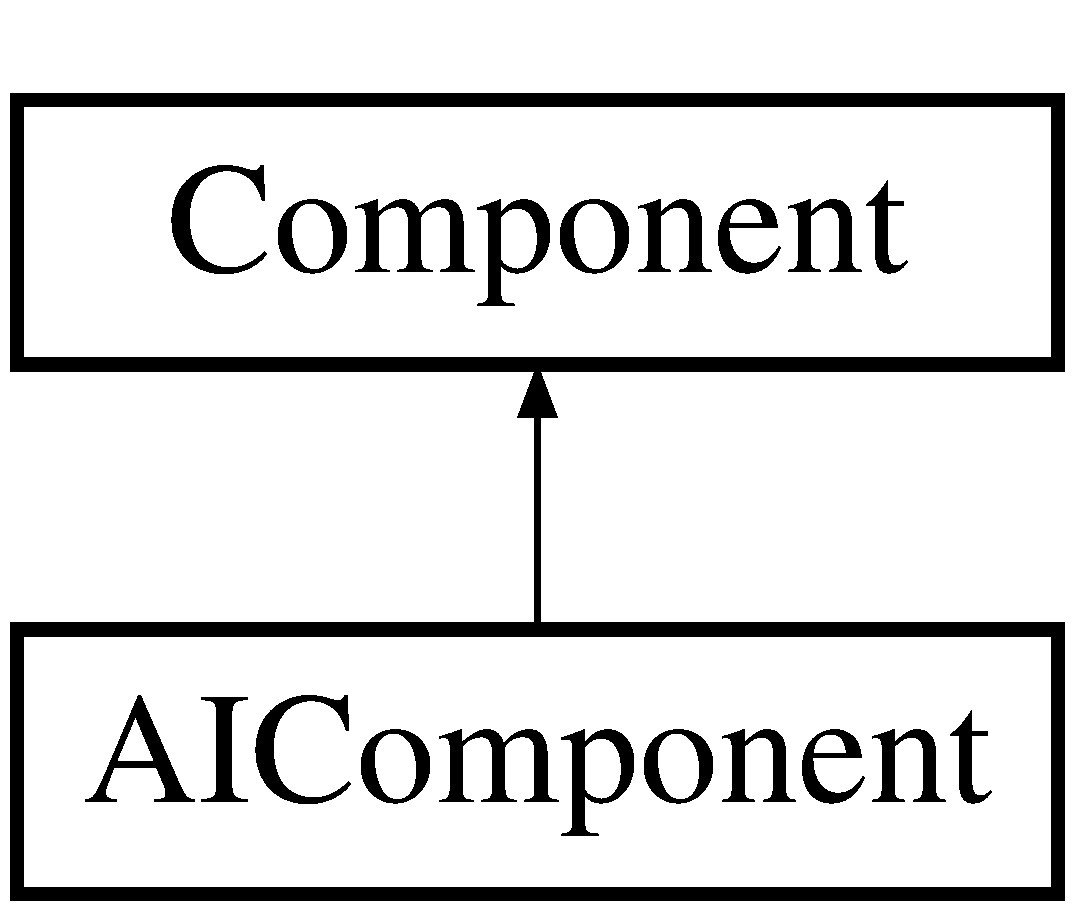
\includegraphics[height=2.000000cm]{class_a_i_component}
\end{center}
\end{figure}
\subsection*{Public Member Functions}
\begin{DoxyCompactItemize}
\item 
\mbox{\hyperlink{class_a_i_component_ac0e093b9d74e3a103d93d843a1795a95}{A\+I\+Component}} ()
\item 
\mbox{\hyperlink{class_a_i_component_a0ffc6db0d1cb5720b8aaef8ec28f4efe}{$\sim$\+A\+I\+Component}} ()
\end{DoxyCompactItemize}
\subsection*{Public Attributes}
\begin{DoxyCompactItemize}
\item 
std\+::unique\+\_\+ptr$<$ \mbox{\hyperlink{class_a_i_behavior}{A\+I\+Behavior}} $>$ \mbox{\hyperlink{class_a_i_component_a39ced78aec7dc4cce01017ad2dfb06ea}{m\+\_\+behavior}}
\end{DoxyCompactItemize}
\subsection*{Additional Inherited Members}


\subsection{Detailed Description}
\mbox{\hyperlink{class_a_i_component}{A\+I\+Component}} is attached to entities to give them AI driven behavior. 

\subsection{Constructor \& Destructor Documentation}
\mbox{\Hypertarget{class_a_i_component_ac0e093b9d74e3a103d93d843a1795a95}\label{class_a_i_component_ac0e093b9d74e3a103d93d843a1795a95}} 
\index{A\+I\+Component@{A\+I\+Component}!A\+I\+Component@{A\+I\+Component}}
\index{A\+I\+Component@{A\+I\+Component}!A\+I\+Component@{A\+I\+Component}}
\subsubsection{\texorpdfstring{A\+I\+Component()}{AIComponent()}}
{\footnotesize\ttfamily A\+I\+Component\+::\+A\+I\+Component (\begin{DoxyParamCaption}{ }\end{DoxyParamCaption})}

Default constructor. \mbox{\Hypertarget{class_a_i_component_a0ffc6db0d1cb5720b8aaef8ec28f4efe}\label{class_a_i_component_a0ffc6db0d1cb5720b8aaef8ec28f4efe}} 
\index{A\+I\+Component@{A\+I\+Component}!````~A\+I\+Component@{$\sim$\+A\+I\+Component}}
\index{````~A\+I\+Component@{$\sim$\+A\+I\+Component}!A\+I\+Component@{A\+I\+Component}}
\subsubsection{\texorpdfstring{$\sim$\+A\+I\+Component()}{~AIComponent()}}
{\footnotesize\ttfamily A\+I\+Component\+::$\sim$\+A\+I\+Component (\begin{DoxyParamCaption}{ }\end{DoxyParamCaption})}

Default destructor. 

\subsection{Member Data Documentation}
\mbox{\Hypertarget{class_a_i_component_a39ced78aec7dc4cce01017ad2dfb06ea}\label{class_a_i_component_a39ced78aec7dc4cce01017ad2dfb06ea}} 
\index{A\+I\+Component@{A\+I\+Component}!m\+\_\+behavior@{m\+\_\+behavior}}
\index{m\+\_\+behavior@{m\+\_\+behavior}!A\+I\+Component@{A\+I\+Component}}
\subsubsection{\texorpdfstring{m\+\_\+behavior}{m\_behavior}}
{\footnotesize\ttfamily std\+::unique\+\_\+ptr$<$\mbox{\hyperlink{class_a_i_behavior}{A\+I\+Behavior}}$>$ A\+I\+Component\+::m\+\_\+behavior}

\mbox{\hyperlink{class_component}{Component}} behavior. 

The documentation for this class was generated from the following files\+:\begin{DoxyCompactItemize}
\item 
Engine/\+Source/\+Runtime/\+A\+I/\mbox{\hyperlink{_a_i_component_8h}{A\+I\+Component.\+h}}\item 
Engine/\+Source/\+Runtime/\+A\+I/\mbox{\hyperlink{_a_i_component_8cpp}{A\+I\+Component.\+cpp}}\end{DoxyCompactItemize}

\hypertarget{class_asset}{}\section{Asset Class Reference}
\label{class_asset}\index{Asset@{Asset}}


{\ttfamily \#include $<$Asset.\+h$>$}

Inheritance diagram for Asset\+:\begin{figure}[H]
\begin{center}
\leavevmode
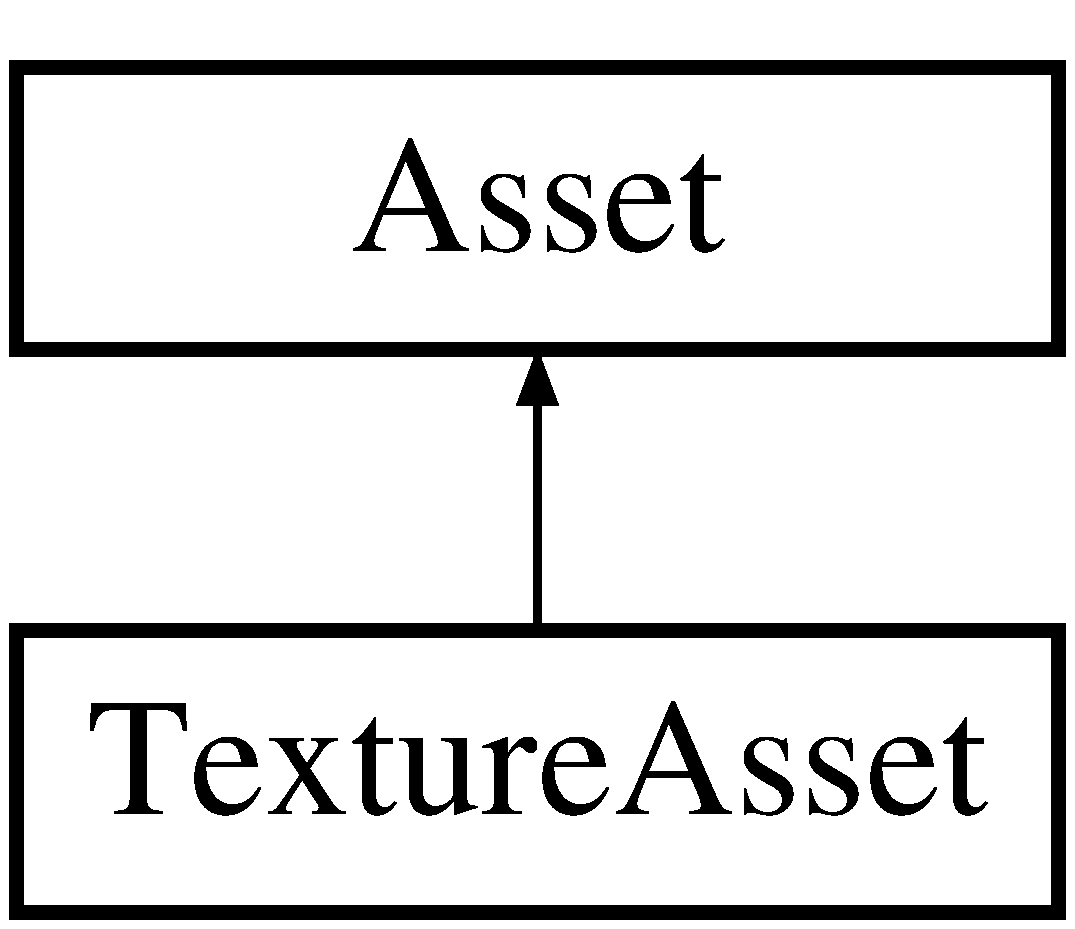
\includegraphics[height=2.000000cm]{class_asset}
\end{center}
\end{figure}
\subsection*{Public Member Functions}
\begin{DoxyCompactItemize}
\item 
\mbox{\hyperlink{class_asset_a1c98c4e76529bc36e1de256d26987e75}{Asset}} (const std\+::string \&asset\+Name)
\item 
virtual \mbox{\hyperlink{class_asset_a46a781917d9ef0be7d6efe79390fe4e6}{$\sim$\+Asset}} ()
\item 
std\+::string \mbox{\hyperlink{class_asset_a7a2d56b7eae0869a5c4fef6a5ca84436}{Get\+Asset\+Name}} () const
\end{DoxyCompactItemize}
\subsection*{Protected Attributes}
\begin{DoxyCompactItemize}
\item 
std\+::string \mbox{\hyperlink{class_asset_a7333657af418ff8386d70be9771d00cc}{m\+\_\+asset\+Name}}
\end{DoxyCompactItemize}


\subsection{Detailed Description}
Interface for an asset object. 

\subsection{Constructor \& Destructor Documentation}
\mbox{\Hypertarget{class_asset_a1c98c4e76529bc36e1de256d26987e75}\label{class_asset_a1c98c4e76529bc36e1de256d26987e75}} 
\index{Asset@{Asset}!Asset@{Asset}}
\index{Asset@{Asset}!Asset@{Asset}}
\subsubsection{\texorpdfstring{Asset()}{Asset()}}
{\footnotesize\ttfamily Asset\+::\+Asset (\begin{DoxyParamCaption}\item[{const std\+::string \&}]{asset\+Name }\end{DoxyParamCaption})}

Constructor. \mbox{\Hypertarget{class_asset_a46a781917d9ef0be7d6efe79390fe4e6}\label{class_asset_a46a781917d9ef0be7d6efe79390fe4e6}} 
\index{Asset@{Asset}!````~Asset@{$\sim$\+Asset}}
\index{````~Asset@{$\sim$\+Asset}!Asset@{Asset}}
\subsubsection{\texorpdfstring{$\sim$\+Asset()}{~Asset()}}
{\footnotesize\ttfamily Asset\+::$\sim$\+Asset (\begin{DoxyParamCaption}{ }\end{DoxyParamCaption})\hspace{0.3cm}{\ttfamily [virtual]}}

Default destructor. 

\subsection{Member Function Documentation}
\mbox{\Hypertarget{class_asset_a7a2d56b7eae0869a5c4fef6a5ca84436}\label{class_asset_a7a2d56b7eae0869a5c4fef6a5ca84436}} 
\index{Asset@{Asset}!Get\+Asset\+Name@{Get\+Asset\+Name}}
\index{Get\+Asset\+Name@{Get\+Asset\+Name}!Asset@{Asset}}
\subsubsection{\texorpdfstring{Get\+Asset\+Name()}{GetAssetName()}}
{\footnotesize\ttfamily std\+::string Asset\+::\+Get\+Asset\+Name (\begin{DoxyParamCaption}{ }\end{DoxyParamCaption}) const\hspace{0.3cm}{\ttfamily [inline]}}

Retunrs the name of the asset. 

\subsection{Member Data Documentation}
\mbox{\Hypertarget{class_asset_a7333657af418ff8386d70be9771d00cc}\label{class_asset_a7333657af418ff8386d70be9771d00cc}} 
\index{Asset@{Asset}!m\+\_\+asset\+Name@{m\+\_\+asset\+Name}}
\index{m\+\_\+asset\+Name@{m\+\_\+asset\+Name}!Asset@{Asset}}
\subsubsection{\texorpdfstring{m\+\_\+asset\+Name}{m\_assetName}}
{\footnotesize\ttfamily std\+::string Asset\+::m\+\_\+asset\+Name\hspace{0.3cm}{\ttfamily [protected]}}

The name of the asset. 

The documentation for this class was generated from the following files\+:\begin{DoxyCompactItemize}
\item 
Engine/\+Source/\+Runtime/\+Resource/\mbox{\hyperlink{_asset_8h}{Asset.\+h}}\item 
Engine/\+Source/\+Runtime/\+Resource/\mbox{\hyperlink{_asset_8cpp}{Asset.\+cpp}}\end{DoxyCompactItemize}

\hypertarget{class_asset_manager}{}\section{Asset\+Manager$<$ T $>$ Class Template Reference}
\label{class_asset_manager}\index{Asset\+Manager$<$ T $>$@{Asset\+Manager$<$ T $>$}}


{\ttfamily \#include $<$Game\+App.\+h$>$}

Inheritance diagram for Asset\+Manager$<$ T $>$\+:\begin{figure}[H]
\begin{center}
\leavevmode
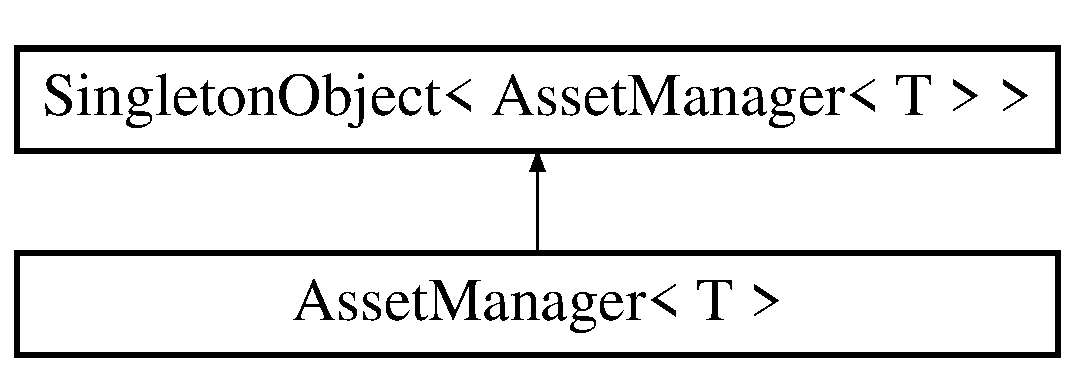
\includegraphics[height=2.000000cm]{class_asset_manager}
\end{center}
\end{figure}
\subsection*{Public Member Functions}
\begin{DoxyCompactItemize}
\item 
\mbox{\hyperlink{class_asset_manager_a17362b22d791f64a200bfeaffa9b5108}{Asset\+Manager}} ()
\item 
\mbox{\hyperlink{class_asset_manager_a99de467c293ead8517bbfd5672b40b0d}{$\sim$\+Asset\+Manager}} ()
\item 
void \mbox{\hyperlink{class_asset_manager_ace92285c403c555e8e6fdb258e9e57d0}{Initialize}} (const std\+::string name)
\item 
std\+::shared\+\_\+ptr$<$ T $>$ \mbox{\hyperlink{class_asset_manager_ad685ea526834b044a13fe07e630bfe0a}{Load}} (const std\+::string \&file\+Path)
\item 
std\+::shared\+\_\+ptr$<$ T $>$ \mbox{\hyperlink{class_asset_manager_a28d1324d3a691d83e4395661702dc9eb}{Get}} (const std\+::string \&file\+Path)
\item 
bool \mbox{\hyperlink{class_asset_manager_a5b015e693d11b39ee98a094ef9d74966}{Un\+Load}} (const std\+::string \&file\+Path)
\item 
const std\+::string \& \mbox{\hyperlink{class_asset_manager_a7c1faafe83a1dbbd1ae463f1de7b6476}{Get\+Asset\+Manager\+Name}} () const
\item 
const int32\+\_\+t \mbox{\hyperlink{class_asset_manager_a329526176de822f96a6b4fb1cb30ce20}{Get\+Size}} () const
\end{DoxyCompactItemize}
\subsection*{Additional Inherited Members}


\subsection{Constructor \& Destructor Documentation}
\mbox{\Hypertarget{class_asset_manager_a17362b22d791f64a200bfeaffa9b5108}\label{class_asset_manager_a17362b22d791f64a200bfeaffa9b5108}} 
\index{Asset\+Manager@{Asset\+Manager}!Asset\+Manager@{Asset\+Manager}}
\index{Asset\+Manager@{Asset\+Manager}!Asset\+Manager@{Asset\+Manager}}
\subsubsection{\texorpdfstring{Asset\+Manager()}{AssetManager()}}
{\footnotesize\ttfamily template$<$class T $>$ \\
\mbox{\hyperlink{class_asset_manager}{Asset\+Manager}}$<$ T $>$\+::\mbox{\hyperlink{class_asset_manager}{Asset\+Manager}} (\begin{DoxyParamCaption}{ }\end{DoxyParamCaption})\hspace{0.3cm}{\ttfamily [inline]}}

Default constructor. \mbox{\Hypertarget{class_asset_manager_a99de467c293ead8517bbfd5672b40b0d}\label{class_asset_manager_a99de467c293ead8517bbfd5672b40b0d}} 
\index{Asset\+Manager@{Asset\+Manager}!````~Asset\+Manager@{$\sim$\+Asset\+Manager}}
\index{````~Asset\+Manager@{$\sim$\+Asset\+Manager}!Asset\+Manager@{Asset\+Manager}}
\subsubsection{\texorpdfstring{$\sim$\+Asset\+Manager()}{~AssetManager()}}
{\footnotesize\ttfamily template$<$class T $>$ \\
\mbox{\hyperlink{class_asset_manager}{Asset\+Manager}}$<$ T $>$\+::$\sim$\mbox{\hyperlink{class_asset_manager}{Asset\+Manager}} (\begin{DoxyParamCaption}{ }\end{DoxyParamCaption})\hspace{0.3cm}{\ttfamily [inline]}}

Default destructor. 

\subsection{Member Function Documentation}
\mbox{\Hypertarget{class_asset_manager_a28d1324d3a691d83e4395661702dc9eb}\label{class_asset_manager_a28d1324d3a691d83e4395661702dc9eb}} 
\index{Asset\+Manager@{Asset\+Manager}!Get@{Get}}
\index{Get@{Get}!Asset\+Manager@{Asset\+Manager}}
\subsubsection{\texorpdfstring{Get()}{Get()}}
{\footnotesize\ttfamily template$<$class T $>$ \\
std\+::shared\+\_\+ptr$<$T$>$ \mbox{\hyperlink{class_asset_manager}{Asset\+Manager}}$<$ T $>$\+::Get (\begin{DoxyParamCaption}\item[{const std\+::string \&}]{file\+Path }\end{DoxyParamCaption})\hspace{0.3cm}{\ttfamily [inline]}}

Returns asset from the map. \mbox{\Hypertarget{class_asset_manager_a7c1faafe83a1dbbd1ae463f1de7b6476}\label{class_asset_manager_a7c1faafe83a1dbbd1ae463f1de7b6476}} 
\index{Asset\+Manager@{Asset\+Manager}!Get\+Asset\+Manager\+Name@{Get\+Asset\+Manager\+Name}}
\index{Get\+Asset\+Manager\+Name@{Get\+Asset\+Manager\+Name}!Asset\+Manager@{Asset\+Manager}}
\subsubsection{\texorpdfstring{Get\+Asset\+Manager\+Name()}{GetAssetManagerName()}}
{\footnotesize\ttfamily template$<$class T $>$ \\
const std\+::string\& \mbox{\hyperlink{class_asset_manager}{Asset\+Manager}}$<$ T $>$\+::Get\+Asset\+Manager\+Name (\begin{DoxyParamCaption}{ }\end{DoxyParamCaption}) const\hspace{0.3cm}{\ttfamily [inline]}}

Returns the name of the asset manager. \mbox{\Hypertarget{class_asset_manager_a329526176de822f96a6b4fb1cb30ce20}\label{class_asset_manager_a329526176de822f96a6b4fb1cb30ce20}} 
\index{Asset\+Manager@{Asset\+Manager}!Get\+Size@{Get\+Size}}
\index{Get\+Size@{Get\+Size}!Asset\+Manager@{Asset\+Manager}}
\subsubsection{\texorpdfstring{Get\+Size()}{GetSize()}}
{\footnotesize\ttfamily template$<$class T $>$ \\
const int32\+\_\+t \mbox{\hyperlink{class_asset_manager}{Asset\+Manager}}$<$ T $>$\+::Get\+Size (\begin{DoxyParamCaption}{ }\end{DoxyParamCaption}) const\hspace{0.3cm}{\ttfamily [inline]}}

Returns the size of the asset manager. \mbox{\Hypertarget{class_asset_manager_ace92285c403c555e8e6fdb258e9e57d0}\label{class_asset_manager_ace92285c403c555e8e6fdb258e9e57d0}} 
\index{Asset\+Manager@{Asset\+Manager}!Initialize@{Initialize}}
\index{Initialize@{Initialize}!Asset\+Manager@{Asset\+Manager}}
\subsubsection{\texorpdfstring{Initialize()}{Initialize()}}
{\footnotesize\ttfamily template$<$class T $>$ \\
void \mbox{\hyperlink{class_asset_manager}{Asset\+Manager}}$<$ T $>$\+::Initialize (\begin{DoxyParamCaption}\item[{const std\+::string}]{name }\end{DoxyParamCaption})\hspace{0.3cm}{\ttfamily [inline]}}

Initialize the asset manager. \mbox{\Hypertarget{class_asset_manager_ad685ea526834b044a13fe07e630bfe0a}\label{class_asset_manager_ad685ea526834b044a13fe07e630bfe0a}} 
\index{Asset\+Manager@{Asset\+Manager}!Load@{Load}}
\index{Load@{Load}!Asset\+Manager@{Asset\+Manager}}
\subsubsection{\texorpdfstring{Load()}{Load()}}
{\footnotesize\ttfamily template$<$class T $>$ \\
std\+::shared\+\_\+ptr$<$T$>$ \mbox{\hyperlink{class_asset_manager}{Asset\+Manager}}$<$ T $>$\+::Load (\begin{DoxyParamCaption}\item[{const std\+::string \&}]{file\+Path }\end{DoxyParamCaption})\hspace{0.3cm}{\ttfamily [inline]}}

Load an asset into the asset manager. \mbox{\Hypertarget{class_asset_manager_a5b015e693d11b39ee98a094ef9d74966}\label{class_asset_manager_a5b015e693d11b39ee98a094ef9d74966}} 
\index{Asset\+Manager@{Asset\+Manager}!Un\+Load@{Un\+Load}}
\index{Un\+Load@{Un\+Load}!Asset\+Manager@{Asset\+Manager}}
\subsubsection{\texorpdfstring{Un\+Load()}{UnLoad()}}
{\footnotesize\ttfamily template$<$class T $>$ \\
bool \mbox{\hyperlink{class_asset_manager}{Asset\+Manager}}$<$ T $>$\+::Un\+Load (\begin{DoxyParamCaption}\item[{const std\+::string \&}]{file\+Path }\end{DoxyParamCaption})\hspace{0.3cm}{\ttfamily [inline]}}

Removes an asset from the asset manager. 

The documentation for this class was generated from the following files\+:\begin{DoxyCompactItemize}
\item 
Engine/\+Source/\+Runtime/\+Core/\mbox{\hyperlink{_game_app_8h}{Game\+App.\+h}}\item 
Engine/\+Source/\+Runtime/\+Resource/\mbox{\hyperlink{_asset_manager_8h}{Asset\+Manager.\+h}}\end{DoxyCompactItemize}

\hypertarget{class_audio_cue}{}\section{Audio\+Cue Class Reference}
\label{class_audio_cue}\index{Audio\+Cue@{Audio\+Cue}}


{\ttfamily \#include $<$Audio\+Cue.\+h$>$}

\subsection*{Public Member Functions}
\begin{DoxyCompactItemize}
\item 
\mbox{\hyperlink{class_audio_cue_a5a28ab84a790e98e67fc433b117fb71d}{Audio\+Cue}} ()
\item 
\mbox{\hyperlink{class_audio_cue_a0055a983611df3b4581fe88bcb3c7505}{$\sim$\+Audio\+Cue}} ()
\end{DoxyCompactItemize}


\subsection{Detailed Description}
\mbox{\hyperlink{class_audio_cue}{Audio\+Cue}} is used to play and control sounds. 

\subsection{Constructor \& Destructor Documentation}
\mbox{\Hypertarget{class_audio_cue_a5a28ab84a790e98e67fc433b117fb71d}\label{class_audio_cue_a5a28ab84a790e98e67fc433b117fb71d}} 
\index{Audio\+Cue@{Audio\+Cue}!Audio\+Cue@{Audio\+Cue}}
\index{Audio\+Cue@{Audio\+Cue}!Audio\+Cue@{Audio\+Cue}}
\subsubsection{\texorpdfstring{Audio\+Cue()}{AudioCue()}}
{\footnotesize\ttfamily Audio\+Cue\+::\+Audio\+Cue (\begin{DoxyParamCaption}{ }\end{DoxyParamCaption})}

Default constructor. \mbox{\Hypertarget{class_audio_cue_a0055a983611df3b4581fe88bcb3c7505}\label{class_audio_cue_a0055a983611df3b4581fe88bcb3c7505}} 
\index{Audio\+Cue@{Audio\+Cue}!````~Audio\+Cue@{$\sim$\+Audio\+Cue}}
\index{````~Audio\+Cue@{$\sim$\+Audio\+Cue}!Audio\+Cue@{Audio\+Cue}}
\subsubsection{\texorpdfstring{$\sim$\+Audio\+Cue()}{~AudioCue()}}
{\footnotesize\ttfamily Audio\+Cue\+::$\sim$\+Audio\+Cue (\begin{DoxyParamCaption}{ }\end{DoxyParamCaption})}

Default destructor. 

The documentation for this class was generated from the following files\+:\begin{DoxyCompactItemize}
\item 
Engine/\+Source/\+Runtime/\+Audio/\mbox{\hyperlink{_audio_cue_8h}{Audio\+Cue.\+h}}\item 
Engine/\+Source/\+Runtime/\+Audio/\mbox{\hyperlink{_audio_cue_8cpp}{Audio\+Cue.\+cpp}}\end{DoxyCompactItemize}

\hypertarget{class_audio_manager}{}\section{Audio\+Manager Class Reference}
\label{class_audio_manager}\index{Audio\+Manager@{Audio\+Manager}}


{\ttfamily \#include $<$Audio\+Manager.\+h$>$}

\subsection*{Public Member Functions}
\begin{DoxyCompactItemize}
\item 
\mbox{\hyperlink{class_audio_manager_ace4284dab1ad87e26b177dc57a7d357d}{Audio\+Manager}} (\mbox{\hyperlink{class_world}{World}} $\ast$world)
\item 
\mbox{\hyperlink{class_audio_manager_ad94dc46723c6d7cf8c81fc3772a842aa}{$\sim$\+Audio\+Manager}} ()
\item 
void \mbox{\hyperlink{class_audio_manager_a503509b0f62bd768f59f543bd52687d6}{Initilaize}} ()
\item 
void \mbox{\hyperlink{class_audio_manager_a8956677aeb7abb69b5254c2a89315f9f}{Shutdown}} ()
\item 
void \mbox{\hyperlink{class_audio_manager_a4dad07a2544905f1fd94fb4e2e4a34fc}{Update}} ()
\end{DoxyCompactItemize}


\subsection{Detailed Description}
Class for managing audio systems. 

\subsection{Constructor \& Destructor Documentation}
\mbox{\Hypertarget{class_audio_manager_ace4284dab1ad87e26b177dc57a7d357d}\label{class_audio_manager_ace4284dab1ad87e26b177dc57a7d357d}} 
\index{Audio\+Manager@{Audio\+Manager}!Audio\+Manager@{Audio\+Manager}}
\index{Audio\+Manager@{Audio\+Manager}!Audio\+Manager@{Audio\+Manager}}
\subsubsection{\texorpdfstring{Audio\+Manager()}{AudioManager()}}
{\footnotesize\ttfamily Audio\+Manager\+::\+Audio\+Manager (\begin{DoxyParamCaption}\item[{\mbox{\hyperlink{class_world}{World}} $\ast$}]{world }\end{DoxyParamCaption})}

Default constructor. \mbox{\Hypertarget{class_audio_manager_ad94dc46723c6d7cf8c81fc3772a842aa}\label{class_audio_manager_ad94dc46723c6d7cf8c81fc3772a842aa}} 
\index{Audio\+Manager@{Audio\+Manager}!````~Audio\+Manager@{$\sim$\+Audio\+Manager}}
\index{````~Audio\+Manager@{$\sim$\+Audio\+Manager}!Audio\+Manager@{Audio\+Manager}}
\subsubsection{\texorpdfstring{$\sim$\+Audio\+Manager()}{~AudioManager()}}
{\footnotesize\ttfamily Audio\+Manager\+::$\sim$\+Audio\+Manager (\begin{DoxyParamCaption}{ }\end{DoxyParamCaption})}

Default destructor. 

\subsection{Member Function Documentation}
\mbox{\Hypertarget{class_audio_manager_a503509b0f62bd768f59f543bd52687d6}\label{class_audio_manager_a503509b0f62bd768f59f543bd52687d6}} 
\index{Audio\+Manager@{Audio\+Manager}!Initilaize@{Initilaize}}
\index{Initilaize@{Initilaize}!Audio\+Manager@{Audio\+Manager}}
\subsubsection{\texorpdfstring{Initilaize()}{Initilaize()}}
{\footnotesize\ttfamily void Audio\+Manager\+::\+Initilaize (\begin{DoxyParamCaption}{ }\end{DoxyParamCaption})}

Initializes audio systems. \mbox{\Hypertarget{class_audio_manager_a8956677aeb7abb69b5254c2a89315f9f}\label{class_audio_manager_a8956677aeb7abb69b5254c2a89315f9f}} 
\index{Audio\+Manager@{Audio\+Manager}!Shutdown@{Shutdown}}
\index{Shutdown@{Shutdown}!Audio\+Manager@{Audio\+Manager}}
\subsubsection{\texorpdfstring{Shutdown()}{Shutdown()}}
{\footnotesize\ttfamily void Audio\+Manager\+::\+Shutdown (\begin{DoxyParamCaption}{ }\end{DoxyParamCaption})}

Shutdown audio systems. \mbox{\Hypertarget{class_audio_manager_a4dad07a2544905f1fd94fb4e2e4a34fc}\label{class_audio_manager_a4dad07a2544905f1fd94fb4e2e4a34fc}} 
\index{Audio\+Manager@{Audio\+Manager}!Update@{Update}}
\index{Update@{Update}!Audio\+Manager@{Audio\+Manager}}
\subsubsection{\texorpdfstring{Update()}{Update()}}
{\footnotesize\ttfamily void Audio\+Manager\+::\+Update (\begin{DoxyParamCaption}{ }\end{DoxyParamCaption})}

Update audio systems, called once per frame. 

The documentation for this class was generated from the following files\+:\begin{DoxyCompactItemize}
\item 
Engine/\+Source/\+Runtime/\+Audio/\mbox{\hyperlink{_audio_manager_8h}{Audio\+Manager.\+h}}\item 
Engine/\+Source/\+Runtime/\+Audio/\mbox{\hyperlink{_audio_manager_8cpp}{Audio\+Manager.\+cpp}}\end{DoxyCompactItemize}

\hypertarget{class_collision_component}{}\section{Collision\+Component Class Reference}
\label{class_collision_component}\index{Collision\+Component@{Collision\+Component}}


{\ttfamily \#include $<$Collision\+Component.\+h$>$}

Inheritance diagram for Collision\+Component\+:\begin{figure}[H]
\begin{center}
\leavevmode
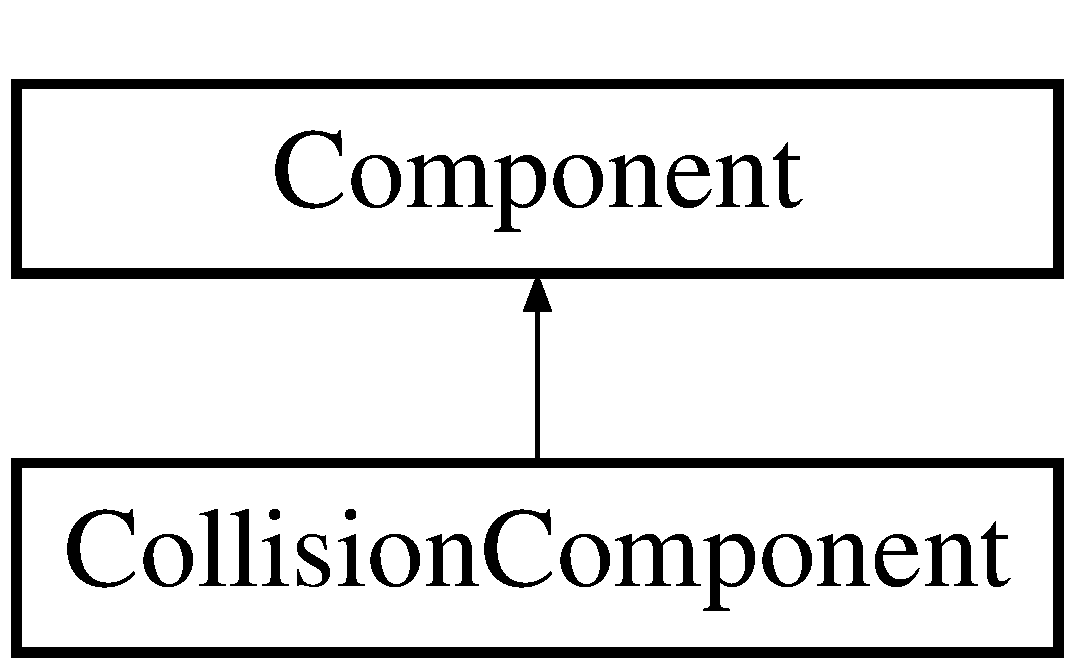
\includegraphics[height=2.000000cm]{class_collision_component}
\end{center}
\end{figure}
\subsection*{Public Member Functions}
\begin{DoxyCompactItemize}
\item 
\mbox{\hyperlink{class_collision_component_a85c7ca3d9925b6c4bda8c8a2a6140aa9}{Collision\+Component}} ()
\item 
\mbox{\hyperlink{class_collision_component_a8927f6bcecb9862b870426af970ab3b7}{$\sim$\+Collision\+Component}} ()
\item 
bool \mbox{\hyperlink{class_collision_component_a612c1e5c553ef889ec5405bd236c4cef}{Intersect}} (const \mbox{\hyperlink{class_collision_component}{Collision\+Component}} \&other\+Comp)
\item 
void \mbox{\hyperlink{class_collision_component_a4bd86e9646160a141aed8a40704ad5fd}{Set\+Radius}} (float radius)
\item 
float \mbox{\hyperlink{class_collision_component_a3645d98e7ed2c6066d4779243b837e9a}{Get\+Radius}} () const
\end{DoxyCompactItemize}
\subsection*{Additional Inherited Members}


\subsection{Constructor \& Destructor Documentation}
\mbox{\Hypertarget{class_collision_component_a85c7ca3d9925b6c4bda8c8a2a6140aa9}\label{class_collision_component_a85c7ca3d9925b6c4bda8c8a2a6140aa9}} 
\index{Collision\+Component@{Collision\+Component}!Collision\+Component@{Collision\+Component}}
\index{Collision\+Component@{Collision\+Component}!Collision\+Component@{Collision\+Component}}
\subsubsection{\texorpdfstring{Collision\+Component()}{CollisionComponent()}}
{\footnotesize\ttfamily Collision\+Component\+::\+Collision\+Component (\begin{DoxyParamCaption}{ }\end{DoxyParamCaption})}

\mbox{\Hypertarget{class_collision_component_a8927f6bcecb9862b870426af970ab3b7}\label{class_collision_component_a8927f6bcecb9862b870426af970ab3b7}} 
\index{Collision\+Component@{Collision\+Component}!````~Collision\+Component@{$\sim$\+Collision\+Component}}
\index{````~Collision\+Component@{$\sim$\+Collision\+Component}!Collision\+Component@{Collision\+Component}}
\subsubsection{\texorpdfstring{$\sim$\+Collision\+Component()}{~CollisionComponent()}}
{\footnotesize\ttfamily Collision\+Component\+::$\sim$\+Collision\+Component (\begin{DoxyParamCaption}{ }\end{DoxyParamCaption})}



\subsection{Member Function Documentation}
\mbox{\Hypertarget{class_collision_component_a3645d98e7ed2c6066d4779243b837e9a}\label{class_collision_component_a3645d98e7ed2c6066d4779243b837e9a}} 
\index{Collision\+Component@{Collision\+Component}!Get\+Radius@{Get\+Radius}}
\index{Get\+Radius@{Get\+Radius}!Collision\+Component@{Collision\+Component}}
\subsubsection{\texorpdfstring{Get\+Radius()}{GetRadius()}}
{\footnotesize\ttfamily float Collision\+Component\+::\+Get\+Radius (\begin{DoxyParamCaption}{ }\end{DoxyParamCaption}) const\hspace{0.3cm}{\ttfamily [inline]}}

\mbox{\Hypertarget{class_collision_component_a612c1e5c553ef889ec5405bd236c4cef}\label{class_collision_component_a612c1e5c553ef889ec5405bd236c4cef}} 
\index{Collision\+Component@{Collision\+Component}!Intersect@{Intersect}}
\index{Intersect@{Intersect}!Collision\+Component@{Collision\+Component}}
\subsubsection{\texorpdfstring{Intersect()}{Intersect()}}
{\footnotesize\ttfamily bool Collision\+Component\+::\+Intersect (\begin{DoxyParamCaption}\item[{const \mbox{\hyperlink{class_collision_component}{Collision\+Component}} \&}]{other\+Comp }\end{DoxyParamCaption})}

\mbox{\Hypertarget{class_collision_component_a4bd86e9646160a141aed8a40704ad5fd}\label{class_collision_component_a4bd86e9646160a141aed8a40704ad5fd}} 
\index{Collision\+Component@{Collision\+Component}!Set\+Radius@{Set\+Radius}}
\index{Set\+Radius@{Set\+Radius}!Collision\+Component@{Collision\+Component}}
\subsubsection{\texorpdfstring{Set\+Radius()}{SetRadius()}}
{\footnotesize\ttfamily void Collision\+Component\+::\+Set\+Radius (\begin{DoxyParamCaption}\item[{float}]{radius }\end{DoxyParamCaption})}



The documentation for this class was generated from the following files\+:\begin{DoxyCompactItemize}
\item 
Engine/\+Source/\+Runtime/\+Game\+Object/\+Components/\mbox{\hyperlink{_collision_component_8h}{Collision\+Component.\+h}}\item 
Engine/\+Source/\+Runtime/\+Game\+Object/\+Components/\mbox{\hyperlink{_collision_component_8cpp}{Collision\+Component.\+cpp}}\end{DoxyCompactItemize}

\hypertarget{class_component}{}\section{Component Class Reference}
\label{class_component}\index{Component@{Component}}


{\ttfamily \#include $<$Component.\+h$>$}

Inheritance diagram for Component\+:\begin{figure}[H]
\begin{center}
\leavevmode
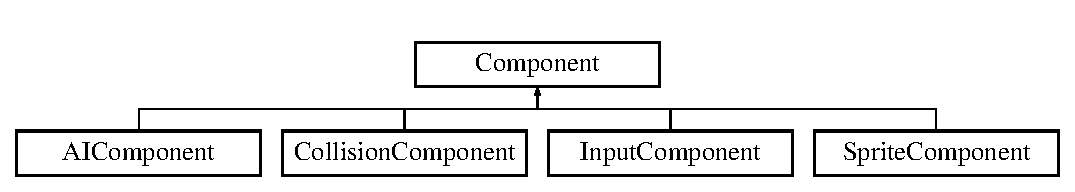
\includegraphics[height=2.000000cm]{class_component}
\end{center}
\end{figure}
\subsection*{Public Member Functions}
\begin{DoxyCompactItemize}
\item 
\mbox{\hyperlink{class_component_a8775db6d1a2c1afc2e77cd3c8f39da6f}{Component}} ()
\item 
virtual \mbox{\hyperlink{class_component_ab8378fa275af98e568a7e91d33d867af}{$\sim$\+Component}} ()
\item 
virtual void \mbox{\hyperlink{class_component_a65053e7e92ff6344e6b028111e43c3c9}{Initialize\+Component}} ()
\item 
virtual void \mbox{\hyperlink{class_component_a7866088cbcf6713821951955eadc85ce}{Pre\+Update}} ()
\item 
virtual void \mbox{\hyperlink{class_component_a8afb7c9504f763728bfedf642cfc5f43}{Update\+Component}} (float delta\+Time)
\item 
void \mbox{\hyperlink{class_component_adccde1de0f593815f081c7df620becbe}{Enable\+Component}} ()
\item 
void \mbox{\hyperlink{class_component_abe8c32edb2ca2b367223ed1f183dc512}{Disable\+Component}} ()
\item 
void \mbox{\hyperlink{class_component_afe37d738fe82aa6b77d7e7398651aa78}{Set\+Owner}} (\mbox{\hyperlink{class_entity}{Entity}} $\ast$new\+Owner)
\item 
bool \mbox{\hyperlink{class_component_acc8b4b096202b1b981973eee31bd682e}{Get\+Is\+Active}} () const
\item 
\mbox{\hyperlink{class_entity}{Entity}} $\ast$ \mbox{\hyperlink{class_component_a7bd8639dadfcaef6baaff8c3b17ae5e6}{Get\+Entity\+Owner}} () const
\end{DoxyCompactItemize}
\subsection*{Protected Attributes}
\begin{DoxyCompactItemize}
\item 
\mbox{\hyperlink{class_entity}{Entity}} $\ast$ \mbox{\hyperlink{class_component_a98e6a9c221fbd50fe38567a48d0da17e}{m\+\_\+entity\+Owner}}
\item 
bool \mbox{\hyperlink{class_component_a6ed72c25c8ea738ebc5a69c66728bf60}{m\+\_\+is\+Active}}
\end{DoxyCompactItemize}


\subsection{Detailed Description}
\mbox{\hyperlink{class_component}{Component}} is a base class for all components that can be attached to entities. 

\subsection{Constructor \& Destructor Documentation}
\mbox{\Hypertarget{class_component_a8775db6d1a2c1afc2e77cd3c8f39da6f}\label{class_component_a8775db6d1a2c1afc2e77cd3c8f39da6f}} 
\index{Component@{Component}!Component@{Component}}
\index{Component@{Component}!Component@{Component}}
\subsubsection{\texorpdfstring{Component()}{Component()}}
{\footnotesize\ttfamily Component\+::\+Component (\begin{DoxyParamCaption}{ }\end{DoxyParamCaption})}

Default constructor. \mbox{\Hypertarget{class_component_ab8378fa275af98e568a7e91d33d867af}\label{class_component_ab8378fa275af98e568a7e91d33d867af}} 
\index{Component@{Component}!````~Component@{$\sim$\+Component}}
\index{````~Component@{$\sim$\+Component}!Component@{Component}}
\subsubsection{\texorpdfstring{$\sim$\+Component()}{~Component()}}
{\footnotesize\ttfamily Component\+::$\sim$\+Component (\begin{DoxyParamCaption}{ }\end{DoxyParamCaption})\hspace{0.3cm}{\ttfamily [virtual]}}

Default destructor. 

\subsection{Member Function Documentation}
\mbox{\Hypertarget{class_component_abe8c32edb2ca2b367223ed1f183dc512}\label{class_component_abe8c32edb2ca2b367223ed1f183dc512}} 
\index{Component@{Component}!Disable\+Component@{Disable\+Component}}
\index{Disable\+Component@{Disable\+Component}!Component@{Component}}
\subsubsection{\texorpdfstring{Disable\+Component()}{DisableComponent()}}
{\footnotesize\ttfamily void Component\+::\+Disable\+Component (\begin{DoxyParamCaption}{ }\end{DoxyParamCaption})}

Disable this component. \mbox{\Hypertarget{class_component_adccde1de0f593815f081c7df620becbe}\label{class_component_adccde1de0f593815f081c7df620becbe}} 
\index{Component@{Component}!Enable\+Component@{Enable\+Component}}
\index{Enable\+Component@{Enable\+Component}!Component@{Component}}
\subsubsection{\texorpdfstring{Enable\+Component()}{EnableComponent()}}
{\footnotesize\ttfamily void Component\+::\+Enable\+Component (\begin{DoxyParamCaption}{ }\end{DoxyParamCaption})}

Enable this component. \mbox{\Hypertarget{class_component_a7bd8639dadfcaef6baaff8c3b17ae5e6}\label{class_component_a7bd8639dadfcaef6baaff8c3b17ae5e6}} 
\index{Component@{Component}!Get\+Entity\+Owner@{Get\+Entity\+Owner}}
\index{Get\+Entity\+Owner@{Get\+Entity\+Owner}!Component@{Component}}
\subsubsection{\texorpdfstring{Get\+Entity\+Owner()}{GetEntityOwner()}}
{\footnotesize\ttfamily \mbox{\hyperlink{class_entity}{Entity}}$\ast$ Component\+::\+Get\+Entity\+Owner (\begin{DoxyParamCaption}{ }\end{DoxyParamCaption}) const\hspace{0.3cm}{\ttfamily [inline]}}

Returns the entity that owns this component. \mbox{\Hypertarget{class_component_acc8b4b096202b1b981973eee31bd682e}\label{class_component_acc8b4b096202b1b981973eee31bd682e}} 
\index{Component@{Component}!Get\+Is\+Active@{Get\+Is\+Active}}
\index{Get\+Is\+Active@{Get\+Is\+Active}!Component@{Component}}
\subsubsection{\texorpdfstring{Get\+Is\+Active()}{GetIsActive()}}
{\footnotesize\ttfamily bool Component\+::\+Get\+Is\+Active (\begin{DoxyParamCaption}{ }\end{DoxyParamCaption}) const\hspace{0.3cm}{\ttfamily [inline]}}

Returns true if this component is active. \mbox{\Hypertarget{class_component_a65053e7e92ff6344e6b028111e43c3c9}\label{class_component_a65053e7e92ff6344e6b028111e43c3c9}} 
\index{Component@{Component}!Initialize\+Component@{Initialize\+Component}}
\index{Initialize\+Component@{Initialize\+Component}!Component@{Component}}
\subsubsection{\texorpdfstring{Initialize\+Component()}{InitializeComponent()}}
{\footnotesize\ttfamily void Component\+::\+Initialize\+Component (\begin{DoxyParamCaption}{ }\end{DoxyParamCaption})\hspace{0.3cm}{\ttfamily [virtual]}}

Initialize this component. 

Reimplemented in \mbox{\hyperlink{class_input_component_ad4262870839371f79747db5b6faf25a7}{Input\+Component}}, and \mbox{\hyperlink{class_sprite_component_af4040c615bebb4aea20f274f77e36733}{Sprite\+Component}}.

\mbox{\Hypertarget{class_component_a7866088cbcf6713821951955eadc85ce}\label{class_component_a7866088cbcf6713821951955eadc85ce}} 
\index{Component@{Component}!Pre\+Update@{Pre\+Update}}
\index{Pre\+Update@{Pre\+Update}!Component@{Component}}
\subsubsection{\texorpdfstring{Pre\+Update()}{PreUpdate()}}
{\footnotesize\ttfamily void Component\+::\+Pre\+Update (\begin{DoxyParamCaption}{ }\end{DoxyParamCaption})\hspace{0.3cm}{\ttfamily [virtual]}}

Called before the main update function. 

Reimplemented in \mbox{\hyperlink{class_input_component_a99f431a305362899b8a6682b390c8899}{Input\+Component}}.

\mbox{\Hypertarget{class_component_afe37d738fe82aa6b77d7e7398651aa78}\label{class_component_afe37d738fe82aa6b77d7e7398651aa78}} 
\index{Component@{Component}!Set\+Owner@{Set\+Owner}}
\index{Set\+Owner@{Set\+Owner}!Component@{Component}}
\subsubsection{\texorpdfstring{Set\+Owner()}{SetOwner()}}
{\footnotesize\ttfamily void Component\+::\+Set\+Owner (\begin{DoxyParamCaption}\item[{\mbox{\hyperlink{class_entity}{Entity}} $\ast$}]{new\+Owner }\end{DoxyParamCaption})}

Set the owner for this component. \mbox{\Hypertarget{class_component_a8afb7c9504f763728bfedf642cfc5f43}\label{class_component_a8afb7c9504f763728bfedf642cfc5f43}} 
\index{Component@{Component}!Update\+Component@{Update\+Component}}
\index{Update\+Component@{Update\+Component}!Component@{Component}}
\subsubsection{\texorpdfstring{Update\+Component()}{UpdateComponent()}}
{\footnotesize\ttfamily void Component\+::\+Update\+Component (\begin{DoxyParamCaption}\item[{float}]{delta\+Time }\end{DoxyParamCaption})\hspace{0.3cm}{\ttfamily [virtual]}}

Update this component called, called once per frame. 

Reimplemented in \mbox{\hyperlink{class_sprite_component_aba00f9c0ecc0a0de41f271267c5440ff}{Sprite\+Component}}, and \mbox{\hyperlink{class_input_component_a42d3b0dffbedfd8cf62702096780ed4d}{Input\+Component}}.



\subsection{Member Data Documentation}
\mbox{\Hypertarget{class_component_a98e6a9c221fbd50fe38567a48d0da17e}\label{class_component_a98e6a9c221fbd50fe38567a48d0da17e}} 
\index{Component@{Component}!m\+\_\+entity\+Owner@{m\+\_\+entity\+Owner}}
\index{m\+\_\+entity\+Owner@{m\+\_\+entity\+Owner}!Component@{Component}}
\subsubsection{\texorpdfstring{m\+\_\+entity\+Owner}{m\_entityOwner}}
{\footnotesize\ttfamily \mbox{\hyperlink{class_entity}{Entity}}$\ast$ Component\+::m\+\_\+entity\+Owner\hspace{0.3cm}{\ttfamily [protected]}}

\mbox{\hyperlink{class_entity}{Entity}} that owns this component \mbox{\Hypertarget{class_component_a6ed72c25c8ea738ebc5a69c66728bf60}\label{class_component_a6ed72c25c8ea738ebc5a69c66728bf60}} 
\index{Component@{Component}!m\+\_\+is\+Active@{m\+\_\+is\+Active}}
\index{m\+\_\+is\+Active@{m\+\_\+is\+Active}!Component@{Component}}
\subsubsection{\texorpdfstring{m\+\_\+is\+Active}{m\_isActive}}
{\footnotesize\ttfamily bool Component\+::m\+\_\+is\+Active\hspace{0.3cm}{\ttfamily [protected]}}

Is this component active 

The documentation for this class was generated from the following files\+:\begin{DoxyCompactItemize}
\item 
Engine/\+Source/\+Runtime/\+Game\+Object/\mbox{\hyperlink{_component_8h}{Component.\+h}}\item 
Engine/\+Source/\+Runtime/\+Game\+Object/\mbox{\hyperlink{_component_8cpp}{Component.\+cpp}}\end{DoxyCompactItemize}

\hypertarget{class_component_manager}{}\section{Component\+Manager Class Reference}
\label{class_component_manager}\index{Component\+Manager@{Component\+Manager}}


{\ttfamily \#include $<$Component\+Manager.\+h$>$}

\subsection*{Public Member Functions}
\begin{DoxyCompactItemize}
\item 
\mbox{\hyperlink{class_component_manager_addccd94a0556362431571f1f749a1afe}{Component\+Manager}} ()
\item 
\mbox{\hyperlink{class_component_manager_aa4269438ec6e184a60ea15423bb2fb6c}{$\sim$\+Component\+Manager}} ()
\end{DoxyCompactItemize}


\subsection{Detailed Description}
Container class for managing components. 

\subsection{Constructor \& Destructor Documentation}
\mbox{\Hypertarget{class_component_manager_addccd94a0556362431571f1f749a1afe}\label{class_component_manager_addccd94a0556362431571f1f749a1afe}} 
\index{Component\+Manager@{Component\+Manager}!Component\+Manager@{Component\+Manager}}
\index{Component\+Manager@{Component\+Manager}!Component\+Manager@{Component\+Manager}}
\subsubsection{\texorpdfstring{Component\+Manager()}{ComponentManager()}}
{\footnotesize\ttfamily Component\+Manager\+::\+Component\+Manager (\begin{DoxyParamCaption}{ }\end{DoxyParamCaption})}

Default constructor. \mbox{\Hypertarget{class_component_manager_aa4269438ec6e184a60ea15423bb2fb6c}\label{class_component_manager_aa4269438ec6e184a60ea15423bb2fb6c}} 
\index{Component\+Manager@{Component\+Manager}!````~Component\+Manager@{$\sim$\+Component\+Manager}}
\index{````~Component\+Manager@{$\sim$\+Component\+Manager}!Component\+Manager@{Component\+Manager}}
\subsubsection{\texorpdfstring{$\sim$\+Component\+Manager()}{~ComponentManager()}}
{\footnotesize\ttfamily Component\+Manager\+::$\sim$\+Component\+Manager (\begin{DoxyParamCaption}{ }\end{DoxyParamCaption})}

Default destructor. 

The documentation for this class was generated from the following files\+:\begin{DoxyCompactItemize}
\item 
Engine/\+Source/\+Runtime/\+Game\+Object/\mbox{\hyperlink{_component_manager_8h}{Component\+Manager.\+h}}\item 
Engine/\+Source/\+Runtime/\+Game\+Object/\mbox{\hyperlink{_component_manager_8cpp}{Component\+Manager.\+cpp}}\end{DoxyCompactItemize}

\hypertarget{class_entity}{}\section{Entity Class Reference}
\label{class_entity}\index{Entity@{Entity}}


{\ttfamily \#include $<$Entity.\+h$>$}

\subsection*{Public Member Functions}
\begin{DoxyCompactItemize}
\item 
\mbox{\hyperlink{class_entity_a980f368aa07ce358583982821533a54a}{Entity}} ()
\item 
virtual \mbox{\hyperlink{class_entity_adf6d3f7cb1b2ba029b6b048a395cc8ae}{$\sim$\+Entity}} ()
\item 
virtual void \mbox{\hyperlink{class_entity_a29ff4d8c00040f1aa281f2e039256543}{Initialize}} (S\+D\+L\+\_\+\+Renderer $\ast$renderer)
\item 
virtual void \mbox{\hyperlink{class_entity_a64043a3f77405466222ff997e272924f}{Update}} (float delta\+Time)
\item 
virtual void \mbox{\hyperlink{class_entity_aae4367e01c9e539bc016b6ffa8dcf3d5}{Draw}} (S\+D\+L\+\_\+\+Renderer $\ast$renderer)
\item 
void \mbox{\hyperlink{class_entity_ae4af7f884155869ae624c5668d67d4e5}{Add\+Component}} (std\+::type\+\_\+index type, \mbox{\hyperlink{class_component}{Component}} $\ast$comp)
\item 
{\footnotesize template$<$typename T $>$ }\\T $\ast$ \mbox{\hyperlink{class_entity_a0084a74b2e2a363e4d3224d1877b9cf3}{Get\+Component}} ()
\item 
void \mbox{\hyperlink{class_entity_ae4b8c446f4e75b6b531768bc12832276}{Set\+Position}} (\mbox{\hyperlink{struct_vec2}{Vec2}} new\+Position)
\item 
void \mbox{\hyperlink{class_entity_a096b2532f1357c05b7b45deed900ca2a}{Set\+Scale}} (float new\+Scale)
\item 
void \mbox{\hyperlink{class_entity_a83f149284da6f4dba4274de5c37a408c}{Set\+Rotation}} (float new\+Rotation)
\item 
void \mbox{\hyperlink{class_entity_ade1dea9daf20aeaf47fef4f0126a2860}{Set\+Velcity}} (\mbox{\hyperlink{struct_vec2}{Vec2}} new\+Velocity)
\item 
\mbox{\hyperlink{struct_vec2}{Vec2}} \mbox{\hyperlink{class_entity_aed198c25368025ba9ff9768f17f19e9e}{Get\+Position}} () const
\item 
float \mbox{\hyperlink{class_entity_a56a2203cb76f5a4cd8c16f0f8ce18b57}{Get\+Scale}} () const
\item 
float \mbox{\hyperlink{class_entity_ab5e5cf79cf2ce961c23061798488bcc4}{Get\+Rotation}} () const
\item 
\mbox{\hyperlink{struct_vec2}{Vec2}} \mbox{\hyperlink{class_entity_a020e999dbfc6b04eb7981b1f2496c4f1}{Get\+Velocity}} () const
\item 
void \mbox{\hyperlink{class_entity_a3320db922c2e6a1392144e14c3d6af91}{Set\+Type}} (const std\+::string \&type)
\item 
std\+::string \mbox{\hyperlink{class_entity_a906ca5c844298c0258bda83563f925a0}{Get\+Type}} () const
\item 
void \mbox{\hyperlink{class_entity_ad940b54ddb93e1b2cc72012589576478}{Enable}} ()
\item 
void \mbox{\hyperlink{class_entity_a60976526014b5f8d65666cd51740d421}{Disable}} ()
\item 
bool \mbox{\hyperlink{class_entity_a98ee6f61ed846d661e5e660d9f4d7e10}{Get\+Is\+Active}} () const
\end{DoxyCompactItemize}
\subsection*{Protected Attributes}
\begin{DoxyCompactItemize}
\item 
S\+D\+L\+\_\+\+Renderer $\ast$ \mbox{\hyperlink{class_entity_a797ca76b3015996cbeb3225eff168cfa}{m\+\_\+renderer}}
\item 
\mbox{\hyperlink{struct_vec2}{Vec2}} \mbox{\hyperlink{class_entity_af1dc457432910811ea84e53dc1aedffc}{m\+\_\+position}}
\item 
float \mbox{\hyperlink{class_entity_a044400bb406b1494de4013a6df8a5933}{m\+\_\+scale}}
\item 
float \mbox{\hyperlink{class_entity_aa3ffa7fffee42fdf090ce02b56d6f305}{m\+\_\+rotation}}
\item 
\mbox{\hyperlink{struct_vec2}{Vec2}} \mbox{\hyperlink{class_entity_ae284f1957cfefc2bd7fd02812a1ee62e}{m\+\_\+velocity}}
\item 
std\+::string \mbox{\hyperlink{class_entity_ab0e743c5f841392748e675c43d3a33c4}{m\+\_\+type}}
\item 
std\+::map$<$ std\+::type\+\_\+index, \mbox{\hyperlink{class_component}{Component}} $\ast$ $>$ \mbox{\hyperlink{class_entity_a5f53550a89ee6303d64c8de9e3ade02a}{m\+\_\+component\+List}}
\item 
bool \mbox{\hyperlink{class_entity_a1e67bc72cc50f2be6903cfa23b25f3df}{m\+\_\+is\+Active}}
\end{DoxyCompactItemize}


\subsection{Detailed Description}
\mbox{\hyperlink{class_entity}{Entity}} is the base class for all game objects in the game world. 

\subsection{Constructor \& Destructor Documentation}
\mbox{\Hypertarget{class_entity_a980f368aa07ce358583982821533a54a}\label{class_entity_a980f368aa07ce358583982821533a54a}} 
\index{Entity@{Entity}!Entity@{Entity}}
\index{Entity@{Entity}!Entity@{Entity}}
\subsubsection{\texorpdfstring{Entity()}{Entity()}}
{\footnotesize\ttfamily Entity\+::\+Entity (\begin{DoxyParamCaption}{ }\end{DoxyParamCaption})}

Default constructor. \mbox{\Hypertarget{class_entity_adf6d3f7cb1b2ba029b6b048a395cc8ae}\label{class_entity_adf6d3f7cb1b2ba029b6b048a395cc8ae}} 
\index{Entity@{Entity}!````~Entity@{$\sim$\+Entity}}
\index{````~Entity@{$\sim$\+Entity}!Entity@{Entity}}
\subsubsection{\texorpdfstring{$\sim$\+Entity()}{~Entity()}}
{\footnotesize\ttfamily Entity\+::$\sim$\+Entity (\begin{DoxyParamCaption}{ }\end{DoxyParamCaption})\hspace{0.3cm}{\ttfamily [virtual]}}

Default destructor. 

\subsection{Member Function Documentation}
\mbox{\Hypertarget{class_entity_ae4af7f884155869ae624c5668d67d4e5}\label{class_entity_ae4af7f884155869ae624c5668d67d4e5}} 
\index{Entity@{Entity}!Add\+Component@{Add\+Component}}
\index{Add\+Component@{Add\+Component}!Entity@{Entity}}
\subsubsection{\texorpdfstring{Add\+Component()}{AddComponent()}}
{\footnotesize\ttfamily void Entity\+::\+Add\+Component (\begin{DoxyParamCaption}\item[{std\+::type\+\_\+index}]{type,  }\item[{\mbox{\hyperlink{class_component}{Component}} $\ast$}]{comp }\end{DoxyParamCaption})}

Add a component to this entity. \mbox{\Hypertarget{class_entity_a60976526014b5f8d65666cd51740d421}\label{class_entity_a60976526014b5f8d65666cd51740d421}} 
\index{Entity@{Entity}!Disable@{Disable}}
\index{Disable@{Disable}!Entity@{Entity}}
\subsubsection{\texorpdfstring{Disable()}{Disable()}}
{\footnotesize\ttfamily void Entity\+::\+Disable (\begin{DoxyParamCaption}{ }\end{DoxyParamCaption})}

Disable this entity. \mbox{\Hypertarget{class_entity_aae4367e01c9e539bc016b6ffa8dcf3d5}\label{class_entity_aae4367e01c9e539bc016b6ffa8dcf3d5}} 
\index{Entity@{Entity}!Draw@{Draw}}
\index{Draw@{Draw}!Entity@{Entity}}
\subsubsection{\texorpdfstring{Draw()}{Draw()}}
{\footnotesize\ttfamily void Entity\+::\+Draw (\begin{DoxyParamCaption}\item[{S\+D\+L\+\_\+\+Renderer $\ast$}]{renderer }\end{DoxyParamCaption})\hspace{0.3cm}{\ttfamily [virtual]}}

Draw this entity. \mbox{\Hypertarget{class_entity_ad940b54ddb93e1b2cc72012589576478}\label{class_entity_ad940b54ddb93e1b2cc72012589576478}} 
\index{Entity@{Entity}!Enable@{Enable}}
\index{Enable@{Enable}!Entity@{Entity}}
\subsubsection{\texorpdfstring{Enable()}{Enable()}}
{\footnotesize\ttfamily void Entity\+::\+Enable (\begin{DoxyParamCaption}{ }\end{DoxyParamCaption})}

Activate this entity. \mbox{\Hypertarget{class_entity_a0084a74b2e2a363e4d3224d1877b9cf3}\label{class_entity_a0084a74b2e2a363e4d3224d1877b9cf3}} 
\index{Entity@{Entity}!Get\+Component@{Get\+Component}}
\index{Get\+Component@{Get\+Component}!Entity@{Entity}}
\subsubsection{\texorpdfstring{Get\+Component()}{GetComponent()}}
{\footnotesize\ttfamily template$<$typename T $>$ \\
T$\ast$ Entity\+::\+Get\+Component (\begin{DoxyParamCaption}{ }\end{DoxyParamCaption})\hspace{0.3cm}{\ttfamily [inline]}}

Get a component that is attached to this entity. \mbox{\Hypertarget{class_entity_a98ee6f61ed846d661e5e660d9f4d7e10}\label{class_entity_a98ee6f61ed846d661e5e660d9f4d7e10}} 
\index{Entity@{Entity}!Get\+Is\+Active@{Get\+Is\+Active}}
\index{Get\+Is\+Active@{Get\+Is\+Active}!Entity@{Entity}}
\subsubsection{\texorpdfstring{Get\+Is\+Active()}{GetIsActive()}}
{\footnotesize\ttfamily bool Entity\+::\+Get\+Is\+Active (\begin{DoxyParamCaption}{ }\end{DoxyParamCaption}) const\hspace{0.3cm}{\ttfamily [inline]}}

Returns the active state of this entity. \mbox{\Hypertarget{class_entity_aed198c25368025ba9ff9768f17f19e9e}\label{class_entity_aed198c25368025ba9ff9768f17f19e9e}} 
\index{Entity@{Entity}!Get\+Position@{Get\+Position}}
\index{Get\+Position@{Get\+Position}!Entity@{Entity}}
\subsubsection{\texorpdfstring{Get\+Position()}{GetPosition()}}
{\footnotesize\ttfamily \mbox{\hyperlink{struct_vec2}{Vec2}} Entity\+::\+Get\+Position (\begin{DoxyParamCaption}{ }\end{DoxyParamCaption}) const\hspace{0.3cm}{\ttfamily [inline]}}

Returns the position of the entity. \mbox{\Hypertarget{class_entity_ab5e5cf79cf2ce961c23061798488bcc4}\label{class_entity_ab5e5cf79cf2ce961c23061798488bcc4}} 
\index{Entity@{Entity}!Get\+Rotation@{Get\+Rotation}}
\index{Get\+Rotation@{Get\+Rotation}!Entity@{Entity}}
\subsubsection{\texorpdfstring{Get\+Rotation()}{GetRotation()}}
{\footnotesize\ttfamily float Entity\+::\+Get\+Rotation (\begin{DoxyParamCaption}{ }\end{DoxyParamCaption}) const\hspace{0.3cm}{\ttfamily [inline]}}

Returns the rotation of this entity. \mbox{\Hypertarget{class_entity_a56a2203cb76f5a4cd8c16f0f8ce18b57}\label{class_entity_a56a2203cb76f5a4cd8c16f0f8ce18b57}} 
\index{Entity@{Entity}!Get\+Scale@{Get\+Scale}}
\index{Get\+Scale@{Get\+Scale}!Entity@{Entity}}
\subsubsection{\texorpdfstring{Get\+Scale()}{GetScale()}}
{\footnotesize\ttfamily float Entity\+::\+Get\+Scale (\begin{DoxyParamCaption}{ }\end{DoxyParamCaption}) const\hspace{0.3cm}{\ttfamily [inline]}}

Returns the scale of this entity. \mbox{\Hypertarget{class_entity_a906ca5c844298c0258bda83563f925a0}\label{class_entity_a906ca5c844298c0258bda83563f925a0}} 
\index{Entity@{Entity}!Get\+Type@{Get\+Type}}
\index{Get\+Type@{Get\+Type}!Entity@{Entity}}
\subsubsection{\texorpdfstring{Get\+Type()}{GetType()}}
{\footnotesize\ttfamily std\+::string Entity\+::\+Get\+Type (\begin{DoxyParamCaption}{ }\end{DoxyParamCaption}) const\hspace{0.3cm}{\ttfamily [inline]}}

Get the entity type. \mbox{\Hypertarget{class_entity_a020e999dbfc6b04eb7981b1f2496c4f1}\label{class_entity_a020e999dbfc6b04eb7981b1f2496c4f1}} 
\index{Entity@{Entity}!Get\+Velocity@{Get\+Velocity}}
\index{Get\+Velocity@{Get\+Velocity}!Entity@{Entity}}
\subsubsection{\texorpdfstring{Get\+Velocity()}{GetVelocity()}}
{\footnotesize\ttfamily \mbox{\hyperlink{struct_vec2}{Vec2}} Entity\+::\+Get\+Velocity (\begin{DoxyParamCaption}{ }\end{DoxyParamCaption}) const\hspace{0.3cm}{\ttfamily [inline]}}

Returns the velocity of the entity. \mbox{\Hypertarget{class_entity_a29ff4d8c00040f1aa281f2e039256543}\label{class_entity_a29ff4d8c00040f1aa281f2e039256543}} 
\index{Entity@{Entity}!Initialize@{Initialize}}
\index{Initialize@{Initialize}!Entity@{Entity}}
\subsubsection{\texorpdfstring{Initialize()}{Initialize()}}
{\footnotesize\ttfamily void Entity\+::\+Initialize (\begin{DoxyParamCaption}\item[{S\+D\+L\+\_\+\+Renderer $\ast$}]{renderer }\end{DoxyParamCaption})\hspace{0.3cm}{\ttfamily [virtual]}}

Initialize the entity. \mbox{\Hypertarget{class_entity_ae4b8c446f4e75b6b531768bc12832276}\label{class_entity_ae4b8c446f4e75b6b531768bc12832276}} 
\index{Entity@{Entity}!Set\+Position@{Set\+Position}}
\index{Set\+Position@{Set\+Position}!Entity@{Entity}}
\subsubsection{\texorpdfstring{Set\+Position()}{SetPosition()}}
{\footnotesize\ttfamily void Entity\+::\+Set\+Position (\begin{DoxyParamCaption}\item[{\mbox{\hyperlink{struct_vec2}{Vec2}}}]{new\+Position }\end{DoxyParamCaption})}

Set a new position for the entity. \mbox{\Hypertarget{class_entity_a83f149284da6f4dba4274de5c37a408c}\label{class_entity_a83f149284da6f4dba4274de5c37a408c}} 
\index{Entity@{Entity}!Set\+Rotation@{Set\+Rotation}}
\index{Set\+Rotation@{Set\+Rotation}!Entity@{Entity}}
\subsubsection{\texorpdfstring{Set\+Rotation()}{SetRotation()}}
{\footnotesize\ttfamily void Entity\+::\+Set\+Rotation (\begin{DoxyParamCaption}\item[{float}]{new\+Rotation }\end{DoxyParamCaption})}

Set a new rotation for this entity. \mbox{\Hypertarget{class_entity_a096b2532f1357c05b7b45deed900ca2a}\label{class_entity_a096b2532f1357c05b7b45deed900ca2a}} 
\index{Entity@{Entity}!Set\+Scale@{Set\+Scale}}
\index{Set\+Scale@{Set\+Scale}!Entity@{Entity}}
\subsubsection{\texorpdfstring{Set\+Scale()}{SetScale()}}
{\footnotesize\ttfamily void Entity\+::\+Set\+Scale (\begin{DoxyParamCaption}\item[{float}]{new\+Scale }\end{DoxyParamCaption})}

Set a new scale for this entity. \mbox{\Hypertarget{class_entity_a3320db922c2e6a1392144e14c3d6af91}\label{class_entity_a3320db922c2e6a1392144e14c3d6af91}} 
\index{Entity@{Entity}!Set\+Type@{Set\+Type}}
\index{Set\+Type@{Set\+Type}!Entity@{Entity}}
\subsubsection{\texorpdfstring{Set\+Type()}{SetType()}}
{\footnotesize\ttfamily void Entity\+::\+Set\+Type (\begin{DoxyParamCaption}\item[{const std\+::string \&}]{type }\end{DoxyParamCaption})}

Set the entity type. \mbox{\Hypertarget{class_entity_ade1dea9daf20aeaf47fef4f0126a2860}\label{class_entity_ade1dea9daf20aeaf47fef4f0126a2860}} 
\index{Entity@{Entity}!Set\+Velcity@{Set\+Velcity}}
\index{Set\+Velcity@{Set\+Velcity}!Entity@{Entity}}
\subsubsection{\texorpdfstring{Set\+Velcity()}{SetVelcity()}}
{\footnotesize\ttfamily void Entity\+::\+Set\+Velcity (\begin{DoxyParamCaption}\item[{\mbox{\hyperlink{struct_vec2}{Vec2}}}]{new\+Velocity }\end{DoxyParamCaption})}

Set a new velocity for the entity. \mbox{\Hypertarget{class_entity_a64043a3f77405466222ff997e272924f}\label{class_entity_a64043a3f77405466222ff997e272924f}} 
\index{Entity@{Entity}!Update@{Update}}
\index{Update@{Update}!Entity@{Entity}}
\subsubsection{\texorpdfstring{Update()}{Update()}}
{\footnotesize\ttfamily void Entity\+::\+Update (\begin{DoxyParamCaption}\item[{float}]{delta\+Time }\end{DoxyParamCaption})\hspace{0.3cm}{\ttfamily [virtual]}}

Update this entity, called once per frame. 

\subsection{Member Data Documentation}
\mbox{\Hypertarget{class_entity_a5f53550a89ee6303d64c8de9e3ade02a}\label{class_entity_a5f53550a89ee6303d64c8de9e3ade02a}} 
\index{Entity@{Entity}!m\+\_\+component\+List@{m\+\_\+component\+List}}
\index{m\+\_\+component\+List@{m\+\_\+component\+List}!Entity@{Entity}}
\subsubsection{\texorpdfstring{m\+\_\+component\+List}{m\_componentList}}
{\footnotesize\ttfamily std\+::map$<$std\+::type\+\_\+index, \mbox{\hyperlink{class_component}{Component}}$\ast$$>$ Entity\+::m\+\_\+component\+List\hspace{0.3cm}{\ttfamily [protected]}}

Map of components attached to this entity keyed to via their type. \mbox{\Hypertarget{class_entity_a1e67bc72cc50f2be6903cfa23b25f3df}\label{class_entity_a1e67bc72cc50f2be6903cfa23b25f3df}} 
\index{Entity@{Entity}!m\+\_\+is\+Active@{m\+\_\+is\+Active}}
\index{m\+\_\+is\+Active@{m\+\_\+is\+Active}!Entity@{Entity}}
\subsubsection{\texorpdfstring{m\+\_\+is\+Active}{m\_isActive}}
{\footnotesize\ttfamily bool Entity\+::m\+\_\+is\+Active\hspace{0.3cm}{\ttfamily [protected]}}

Flag to activate this entity. \mbox{\Hypertarget{class_entity_af1dc457432910811ea84e53dc1aedffc}\label{class_entity_af1dc457432910811ea84e53dc1aedffc}} 
\index{Entity@{Entity}!m\+\_\+position@{m\+\_\+position}}
\index{m\+\_\+position@{m\+\_\+position}!Entity@{Entity}}
\subsubsection{\texorpdfstring{m\+\_\+position}{m\_position}}
{\footnotesize\ttfamily \mbox{\hyperlink{struct_vec2}{Vec2}} Entity\+::m\+\_\+position\hspace{0.3cm}{\ttfamily [protected]}}

The position of the entity in 2D space. \mbox{\Hypertarget{class_entity_a797ca76b3015996cbeb3225eff168cfa}\label{class_entity_a797ca76b3015996cbeb3225eff168cfa}} 
\index{Entity@{Entity}!m\+\_\+renderer@{m\+\_\+renderer}}
\index{m\+\_\+renderer@{m\+\_\+renderer}!Entity@{Entity}}
\subsubsection{\texorpdfstring{m\+\_\+renderer}{m\_renderer}}
{\footnotesize\ttfamily S\+D\+L\+\_\+\+Renderer$\ast$ Entity\+::m\+\_\+renderer\hspace{0.3cm}{\ttfamily [protected]}}

Cached renderer pointer. \mbox{\Hypertarget{class_entity_aa3ffa7fffee42fdf090ce02b56d6f305}\label{class_entity_aa3ffa7fffee42fdf090ce02b56d6f305}} 
\index{Entity@{Entity}!m\+\_\+rotation@{m\+\_\+rotation}}
\index{m\+\_\+rotation@{m\+\_\+rotation}!Entity@{Entity}}
\subsubsection{\texorpdfstring{m\+\_\+rotation}{m\_rotation}}
{\footnotesize\ttfamily float Entity\+::m\+\_\+rotation\hspace{0.3cm}{\ttfamily [protected]}}

The rotation of this entity in 2D space. \mbox{\Hypertarget{class_entity_a044400bb406b1494de4013a6df8a5933}\label{class_entity_a044400bb406b1494de4013a6df8a5933}} 
\index{Entity@{Entity}!m\+\_\+scale@{m\+\_\+scale}}
\index{m\+\_\+scale@{m\+\_\+scale}!Entity@{Entity}}
\subsubsection{\texorpdfstring{m\+\_\+scale}{m\_scale}}
{\footnotesize\ttfamily float Entity\+::m\+\_\+scale\hspace{0.3cm}{\ttfamily [protected]}}

The scale of this entity in 2D space. \mbox{\Hypertarget{class_entity_ab0e743c5f841392748e675c43d3a33c4}\label{class_entity_ab0e743c5f841392748e675c43d3a33c4}} 
\index{Entity@{Entity}!m\+\_\+type@{m\+\_\+type}}
\index{m\+\_\+type@{m\+\_\+type}!Entity@{Entity}}
\subsubsection{\texorpdfstring{m\+\_\+type}{m\_type}}
{\footnotesize\ttfamily std\+::string Entity\+::m\+\_\+type\hspace{0.3cm}{\ttfamily [protected]}}

The name for this entity. \mbox{\Hypertarget{class_entity_ae284f1957cfefc2bd7fd02812a1ee62e}\label{class_entity_ae284f1957cfefc2bd7fd02812a1ee62e}} 
\index{Entity@{Entity}!m\+\_\+velocity@{m\+\_\+velocity}}
\index{m\+\_\+velocity@{m\+\_\+velocity}!Entity@{Entity}}
\subsubsection{\texorpdfstring{m\+\_\+velocity}{m\_velocity}}
{\footnotesize\ttfamily \mbox{\hyperlink{struct_vec2}{Vec2}} Entity\+::m\+\_\+velocity\hspace{0.3cm}{\ttfamily [protected]}}

The movement velocity of the entity in 2D space. 

The documentation for this class was generated from the following files\+:\begin{DoxyCompactItemize}
\item 
Engine/\+Source/\+Runtime/\+Game\+Object/\mbox{\hyperlink{_entity_8h}{Entity.\+h}}\item 
Engine/\+Source/\+Runtime/\+Game\+Object/\mbox{\hyperlink{_entity_8cpp}{Entity.\+cpp}}\end{DoxyCompactItemize}

\hypertarget{class_entity_manager}{}\section{Entity\+Manager Class Reference}
\label{class_entity_manager}\index{Entity\+Manager@{Entity\+Manager}}


{\ttfamily \#include $<$Entity\+Manager.\+h$>$}

\subsection*{Public Member Functions}
\begin{DoxyCompactItemize}
\item 
\mbox{\hyperlink{class_entity_manager_a7555637657d090171be6ceee8451de0a}{Entity\+Manager}} ()
\item 
\mbox{\hyperlink{class_entity_manager_a71a36c9fb8d579a1a1ec108e0fccf175}{$\sim$\+Entity\+Manager}} ()
\item 
void \mbox{\hyperlink{class_entity_manager_a06dc55d7fe6da1f48ca2a9313c7060e7}{Add\+Entity}} (\mbox{\hyperlink{class_entity}{Entity}} $\ast$entity)
\item 
void \mbox{\hyperlink{class_entity_manager_a0af35630dea63b0b62b1b03fac453a0f}{Initialize}} (S\+D\+L\+\_\+\+Renderer $\ast$renderer)
\item 
void \mbox{\hyperlink{class_entity_manager_a29ee635235a8b76bdf10336d70dbf6ed}{Update}} (float delta\+Time)
\item 
void \mbox{\hyperlink{class_entity_manager_acdea7d35f1b2d2df949f3360c30728ab}{Draw}} (S\+D\+L\+\_\+\+Renderer $\ast$renderer)
\item 
uint64\+\_\+t \mbox{\hyperlink{class_entity_manager_a9657535930969fb7296aa6bb370df1ea}{Get\+Entity\+Count}} () const
\end{DoxyCompactItemize}


\subsection{Detailed Description}
High level class for managing game entities. 

\subsection{Constructor \& Destructor Documentation}
\mbox{\Hypertarget{class_entity_manager_a7555637657d090171be6ceee8451de0a}\label{class_entity_manager_a7555637657d090171be6ceee8451de0a}} 
\index{Entity\+Manager@{Entity\+Manager}!Entity\+Manager@{Entity\+Manager}}
\index{Entity\+Manager@{Entity\+Manager}!Entity\+Manager@{Entity\+Manager}}
\subsubsection{\texorpdfstring{Entity\+Manager()}{EntityManager()}}
{\footnotesize\ttfamily Entity\+Manager\+::\+Entity\+Manager (\begin{DoxyParamCaption}{ }\end{DoxyParamCaption})}

Default constructor. \mbox{\Hypertarget{class_entity_manager_a71a36c9fb8d579a1a1ec108e0fccf175}\label{class_entity_manager_a71a36c9fb8d579a1a1ec108e0fccf175}} 
\index{Entity\+Manager@{Entity\+Manager}!````~Entity\+Manager@{$\sim$\+Entity\+Manager}}
\index{````~Entity\+Manager@{$\sim$\+Entity\+Manager}!Entity\+Manager@{Entity\+Manager}}
\subsubsection{\texorpdfstring{$\sim$\+Entity\+Manager()}{~EntityManager()}}
{\footnotesize\ttfamily Entity\+Manager\+::$\sim$\+Entity\+Manager (\begin{DoxyParamCaption}{ }\end{DoxyParamCaption})}

Default destructor. 

\subsection{Member Function Documentation}
\mbox{\Hypertarget{class_entity_manager_a06dc55d7fe6da1f48ca2a9313c7060e7}\label{class_entity_manager_a06dc55d7fe6da1f48ca2a9313c7060e7}} 
\index{Entity\+Manager@{Entity\+Manager}!Add\+Entity@{Add\+Entity}}
\index{Add\+Entity@{Add\+Entity}!Entity\+Manager@{Entity\+Manager}}
\subsubsection{\texorpdfstring{Add\+Entity()}{AddEntity()}}
{\footnotesize\ttfamily void Entity\+Manager\+::\+Add\+Entity (\begin{DoxyParamCaption}\item[{\mbox{\hyperlink{class_entity}{Entity}} $\ast$}]{entity }\end{DoxyParamCaption})}

Add an entity to the manager. \mbox{\Hypertarget{class_entity_manager_acdea7d35f1b2d2df949f3360c30728ab}\label{class_entity_manager_acdea7d35f1b2d2df949f3360c30728ab}} 
\index{Entity\+Manager@{Entity\+Manager}!Draw@{Draw}}
\index{Draw@{Draw}!Entity\+Manager@{Entity\+Manager}}
\subsubsection{\texorpdfstring{Draw()}{Draw()}}
{\footnotesize\ttfamily void Entity\+Manager\+::\+Draw (\begin{DoxyParamCaption}\item[{S\+D\+L\+\_\+\+Renderer $\ast$}]{renderer }\end{DoxyParamCaption})}

Draw any managed entities. \mbox{\Hypertarget{class_entity_manager_a9657535930969fb7296aa6bb370df1ea}\label{class_entity_manager_a9657535930969fb7296aa6bb370df1ea}} 
\index{Entity\+Manager@{Entity\+Manager}!Get\+Entity\+Count@{Get\+Entity\+Count}}
\index{Get\+Entity\+Count@{Get\+Entity\+Count}!Entity\+Manager@{Entity\+Manager}}
\subsubsection{\texorpdfstring{Get\+Entity\+Count()}{GetEntityCount()}}
{\footnotesize\ttfamily uint64\+\_\+t Entity\+Manager\+::\+Get\+Entity\+Count (\begin{DoxyParamCaption}{ }\end{DoxyParamCaption}) const\hspace{0.3cm}{\ttfamily [inline]}}

Returns the number of manged entities. \mbox{\Hypertarget{class_entity_manager_a0af35630dea63b0b62b1b03fac453a0f}\label{class_entity_manager_a0af35630dea63b0b62b1b03fac453a0f}} 
\index{Entity\+Manager@{Entity\+Manager}!Initialize@{Initialize}}
\index{Initialize@{Initialize}!Entity\+Manager@{Entity\+Manager}}
\subsubsection{\texorpdfstring{Initialize()}{Initialize()}}
{\footnotesize\ttfamily void Entity\+Manager\+::\+Initialize (\begin{DoxyParamCaption}\item[{S\+D\+L\+\_\+\+Renderer $\ast$}]{renderer }\end{DoxyParamCaption})}

Initialize any managed entities. \mbox{\Hypertarget{class_entity_manager_a29ee635235a8b76bdf10336d70dbf6ed}\label{class_entity_manager_a29ee635235a8b76bdf10336d70dbf6ed}} 
\index{Entity\+Manager@{Entity\+Manager}!Update@{Update}}
\index{Update@{Update}!Entity\+Manager@{Entity\+Manager}}
\subsubsection{\texorpdfstring{Update()}{Update()}}
{\footnotesize\ttfamily void Entity\+Manager\+::\+Update (\begin{DoxyParamCaption}\item[{float}]{delta\+Time }\end{DoxyParamCaption})}

Update any managed entities, called once per frame. 

The documentation for this class was generated from the following files\+:\begin{DoxyCompactItemize}
\item 
Engine/\+Source/\+Runtime/\+Game\+Object/\mbox{\hyperlink{_entity_manager_8h}{Entity\+Manager.\+h}}\item 
Engine/\+Source/\+Runtime/\+Game\+Object/\mbox{\hyperlink{_entity_manager_8cpp}{Entity\+Manager.\+cpp}}\end{DoxyCompactItemize}

\hypertarget{class_event}{}\section{Event Class Reference}
\label{class_event}\index{Event@{Event}}


{\ttfamily \#include $<$Event.\+h$>$}

\subsection*{Public Member Functions}
\begin{DoxyCompactItemize}
\item 
\mbox{\hyperlink{class_event_ab7d875af219d0d97a3b1173b576bf65a}{Event}} (int64\+\_\+t event\+ID)
\item 
int64\+\_\+t \mbox{\hyperlink{class_event_a49eec72ca49bb73e1d28a09db8babadd}{Get\+Event\+ID}} () const
\end{DoxyCompactItemize}


\subsection{Constructor \& Destructor Documentation}
\mbox{\Hypertarget{class_event_ab7d875af219d0d97a3b1173b576bf65a}\label{class_event_ab7d875af219d0d97a3b1173b576bf65a}} 
\index{Event@{Event}!Event@{Event}}
\index{Event@{Event}!Event@{Event}}
\subsubsection{\texorpdfstring{Event()}{Event()}}
{\footnotesize\ttfamily Event\+::\+Event (\begin{DoxyParamCaption}\item[{int64\+\_\+t}]{event\+ID }\end{DoxyParamCaption})}



\subsection{Member Function Documentation}
\mbox{\Hypertarget{class_event_a49eec72ca49bb73e1d28a09db8babadd}\label{class_event_a49eec72ca49bb73e1d28a09db8babadd}} 
\index{Event@{Event}!Get\+Event\+ID@{Get\+Event\+ID}}
\index{Get\+Event\+ID@{Get\+Event\+ID}!Event@{Event}}
\subsubsection{\texorpdfstring{Get\+Event\+I\+D()}{GetEventID()}}
{\footnotesize\ttfamily int64\+\_\+t Event\+::\+Get\+Event\+ID (\begin{DoxyParamCaption}{ }\end{DoxyParamCaption}) const\hspace{0.3cm}{\ttfamily [inline]}}



The documentation for this class was generated from the following files\+:\begin{DoxyCompactItemize}
\item 
Engine/\+Source/\+Runtime/\+Event\+System/\mbox{\hyperlink{_event_8h}{Event.\+h}}\item 
Engine/\+Source/\+Runtime/\+Event\+System/\mbox{\hyperlink{_event_8cpp}{Event.\+cpp}}\end{DoxyCompactItemize}

\hypertarget{class_event_dispatcher}{}\section{Event\+Dispatcher Class Reference}
\label{class_event_dispatcher}\index{Event\+Dispatcher@{Event\+Dispatcher}}


{\ttfamily \#include $<$Event\+Dispatcher.\+h$>$}

\subsection*{Public Member Functions}
\begin{DoxyCompactItemize}
\item 
\mbox{\hyperlink{class_event_dispatcher_a4230d150965d1bdf1552b60ea3f6a64a}{Event\+Dispatcher}} (\mbox{\hyperlink{class_event}{Event}} $\ast$event)
\item 
void \mbox{\hyperlink{class_event_dispatcher_a55e223be473ae7557648b85ea2b19f43}{Disptach}} (std\+::function$<$ bool(T \&)$>$ func)
\end{DoxyCompactItemize}


\subsection{Constructor \& Destructor Documentation}
\mbox{\Hypertarget{class_event_dispatcher_a4230d150965d1bdf1552b60ea3f6a64a}\label{class_event_dispatcher_a4230d150965d1bdf1552b60ea3f6a64a}} 
\index{Event\+Dispatcher@{Event\+Dispatcher}!Event\+Dispatcher@{Event\+Dispatcher}}
\index{Event\+Dispatcher@{Event\+Dispatcher}!Event\+Dispatcher@{Event\+Dispatcher}}
\subsubsection{\texorpdfstring{Event\+Dispatcher()}{EventDispatcher()}}
{\footnotesize\ttfamily Event\+Dispatcher\+::\+Event\+Dispatcher (\begin{DoxyParamCaption}\item[{\mbox{\hyperlink{class_event}{Event}} $\ast$}]{event }\end{DoxyParamCaption})\hspace{0.3cm}{\ttfamily [inline]}}



\subsection{Member Function Documentation}
\mbox{\Hypertarget{class_event_dispatcher_a55e223be473ae7557648b85ea2b19f43}\label{class_event_dispatcher_a55e223be473ae7557648b85ea2b19f43}} 
\index{Event\+Dispatcher@{Event\+Dispatcher}!Disptach@{Disptach}}
\index{Disptach@{Disptach}!Event\+Dispatcher@{Event\+Dispatcher}}
\subsubsection{\texorpdfstring{Disptach()}{Disptach()}}
{\footnotesize\ttfamily void Event\+Dispatcher\+::\+Disptach (\begin{DoxyParamCaption}\item[{std\+::function$<$ bool(T \&)$>$}]{func }\end{DoxyParamCaption})\hspace{0.3cm}{\ttfamily [inline]}}



The documentation for this class was generated from the following file\+:\begin{DoxyCompactItemize}
\item 
Engine/\+Source/\+Runtime/\+Event\+System/\mbox{\hyperlink{_event_dispatcher_8h}{Event\+Dispatcher.\+h}}\end{DoxyCompactItemize}

\hypertarget{class_game_app}{}\section{Game\+App Class Reference}
\label{class_game_app}\index{Game\+App@{Game\+App}}


{\ttfamily \#include $<$Game\+App.\+h$>$}

\subsection*{Public Member Functions}
\begin{DoxyCompactItemize}
\item 
\mbox{\hyperlink{class_game_app_a60fa14c5e72ac86d85257732494210ce}{Game\+App}} ()
\item 
\mbox{\hyperlink{class_game_app_ae23ced12f4a79184b3719b3905c58170}{$\sim$\+Game\+App}} ()
\item 
virtual void \mbox{\hyperlink{class_game_app_a9d9218c197e35c45cd0027f109dcd6a2}{Startup}} ()
\item 
virtual void \mbox{\hyperlink{class_game_app_a0dc0f7396813debb806c16d79efcb111}{Shutdown}} ()
\item 
virtual void \mbox{\hyperlink{class_game_app_af48020622e6db3aa8e55458c3abdff87}{Update}} (float delta\+Time)
\item 
void \mbox{\hyperlink{class_game_app_a62c5268bda2f50c7535848cd21c884b4}{Process\+Events}} ()
\item 
bool \mbox{\hyperlink{class_game_app_aabc1e7e91c577c681c1ef8e45b926286}{Get\+Is\+Running}} () const
\item 
S\+D\+L\+\_\+\+Window $\ast$ \mbox{\hyperlink{class_game_app_a08fc92ae5300a57c05f7bafefa53b82e}{Get\+Window}} () const
\end{DoxyCompactItemize}


\subsection{Detailed Description}
Abstraction layer for a game application. 

\subsection{Constructor \& Destructor Documentation}
\mbox{\Hypertarget{class_game_app_a60fa14c5e72ac86d85257732494210ce}\label{class_game_app_a60fa14c5e72ac86d85257732494210ce}} 
\index{Game\+App@{Game\+App}!Game\+App@{Game\+App}}
\index{Game\+App@{Game\+App}!Game\+App@{Game\+App}}
\subsubsection{\texorpdfstring{Game\+App()}{GameApp()}}
{\footnotesize\ttfamily Game\+App\+::\+Game\+App (\begin{DoxyParamCaption}{ }\end{DoxyParamCaption})}

Default \mbox{\hyperlink{class_game_app}{Game\+App}} constructor. \mbox{\Hypertarget{class_game_app_ae23ced12f4a79184b3719b3905c58170}\label{class_game_app_ae23ced12f4a79184b3719b3905c58170}} 
\index{Game\+App@{Game\+App}!````~Game\+App@{$\sim$\+Game\+App}}
\index{````~Game\+App@{$\sim$\+Game\+App}!Game\+App@{Game\+App}}
\subsubsection{\texorpdfstring{$\sim$\+Game\+App()}{~GameApp()}}
{\footnotesize\ttfamily Game\+App\+::$\sim$\+Game\+App (\begin{DoxyParamCaption}{ }\end{DoxyParamCaption})}

Default \mbox{\hyperlink{class_game_app}{Game\+App}} destructor. 

\subsection{Member Function Documentation}
\mbox{\Hypertarget{class_game_app_aabc1e7e91c577c681c1ef8e45b926286}\label{class_game_app_aabc1e7e91c577c681c1ef8e45b926286}} 
\index{Game\+App@{Game\+App}!Get\+Is\+Running@{Get\+Is\+Running}}
\index{Get\+Is\+Running@{Get\+Is\+Running}!Game\+App@{Game\+App}}
\subsubsection{\texorpdfstring{Get\+Is\+Running()}{GetIsRunning()}}
{\footnotesize\ttfamily bool Game\+App\+::\+Get\+Is\+Running (\begin{DoxyParamCaption}{ }\end{DoxyParamCaption}) const\hspace{0.3cm}{\ttfamily [inline]}}

Returns true if the application is currently running. \mbox{\Hypertarget{class_game_app_a08fc92ae5300a57c05f7bafefa53b82e}\label{class_game_app_a08fc92ae5300a57c05f7bafefa53b82e}} 
\index{Game\+App@{Game\+App}!Get\+Window@{Get\+Window}}
\index{Get\+Window@{Get\+Window}!Game\+App@{Game\+App}}
\subsubsection{\texorpdfstring{Get\+Window()}{GetWindow()}}
{\footnotesize\ttfamily S\+D\+L\+\_\+\+Window$\ast$ Game\+App\+::\+Get\+Window (\begin{DoxyParamCaption}{ }\end{DoxyParamCaption}) const\hspace{0.3cm}{\ttfamily [inline]}}

Returns a pointer to the native window. \mbox{\Hypertarget{class_game_app_a62c5268bda2f50c7535848cd21c884b4}\label{class_game_app_a62c5268bda2f50c7535848cd21c884b4}} 
\index{Game\+App@{Game\+App}!Process\+Events@{Process\+Events}}
\index{Process\+Events@{Process\+Events}!Game\+App@{Game\+App}}
\subsubsection{\texorpdfstring{Process\+Events()}{ProcessEvents()}}
{\footnotesize\ttfamily void Game\+App\+::\+Process\+Events (\begin{DoxyParamCaption}{ }\end{DoxyParamCaption})}

Handles application messages. \mbox{\Hypertarget{class_game_app_a0dc0f7396813debb806c16d79efcb111}\label{class_game_app_a0dc0f7396813debb806c16d79efcb111}} 
\index{Game\+App@{Game\+App}!Shutdown@{Shutdown}}
\index{Shutdown@{Shutdown}!Game\+App@{Game\+App}}
\subsubsection{\texorpdfstring{Shutdown()}{Shutdown()}}
{\footnotesize\ttfamily void Game\+App\+::\+Shutdown (\begin{DoxyParamCaption}{ }\end{DoxyParamCaption})\hspace{0.3cm}{\ttfamily [virtual]}}

Destroys the application. \mbox{\Hypertarget{class_game_app_a9d9218c197e35c45cd0027f109dcd6a2}\label{class_game_app_a9d9218c197e35c45cd0027f109dcd6a2}} 
\index{Game\+App@{Game\+App}!Startup@{Startup}}
\index{Startup@{Startup}!Game\+App@{Game\+App}}
\subsubsection{\texorpdfstring{Startup()}{Startup()}}
{\footnotesize\ttfamily void Game\+App\+::\+Startup (\begin{DoxyParamCaption}{ }\end{DoxyParamCaption})\hspace{0.3cm}{\ttfamily [virtual]}}

Initialize the application state. \mbox{\Hypertarget{class_game_app_af48020622e6db3aa8e55458c3abdff87}\label{class_game_app_af48020622e6db3aa8e55458c3abdff87}} 
\index{Game\+App@{Game\+App}!Update@{Update}}
\index{Update@{Update}!Game\+App@{Game\+App}}
\subsubsection{\texorpdfstring{Update()}{Update()}}
{\footnotesize\ttfamily void Game\+App\+::\+Update (\begin{DoxyParamCaption}\item[{float}]{delta\+Time }\end{DoxyParamCaption})\hspace{0.3cm}{\ttfamily [virtual]}}

Updates the application, called once per frame. 

The documentation for this class was generated from the following files\+:\begin{DoxyCompactItemize}
\item 
Engine/\+Source/\+Runtime/\+Core/\mbox{\hyperlink{_game_app_8h}{Game\+App.\+h}}\item 
Engine/\+Source/\+Runtime/\+Core/\mbox{\hyperlink{_game_app_8cpp}{Game\+App.\+cpp}}\end{DoxyCompactItemize}

\hypertarget{class_gamepad}{}\section{Gamepad Class Reference}
\label{class_gamepad}\index{Gamepad@{Gamepad}}


{\ttfamily \#include $<$Gamepad.\+h$>$}

\subsection*{Public Member Functions}
\begin{DoxyCompactItemize}
\item 
\mbox{\hyperlink{class_gamepad_a766fe5c4b0971cd755f7c930ede3c068}{Gamepad}} ()
\item 
\mbox{\hyperlink{class_gamepad_a5d488c36c656a0f52787671b9b156822}{$\sim$\+Gamepad}} ()
\item 
void \mbox{\hyperlink{class_gamepad_a265afcd224a5f19b76b70c4a27b43cf3}{Initialize}} ()
\item 
void \mbox{\hyperlink{class_gamepad_aa53820795fc6ae0c38b495f90e730fa7}{Pre\+Update}} ()
\item 
void \mbox{\hyperlink{class_gamepad_aade3185158726ef97b588f8c58cb9f8e}{Update}} ()
\item 
void \mbox{\hyperlink{class_gamepad_ad37c0c811ab6d486c64a27ec518d8ec9}{Destroy}} ()
\item 
void \mbox{\hyperlink{class_gamepad_a864978b3a8913f60ac17addb092e07be}{Handle\+Gamepad\+Events}} (S\+D\+L\+\_\+\+Event event)
\item 
bool \mbox{\hyperlink{class_gamepad_a247cbc78f48a4a87c95c5f4909b466c7}{Is\+Button\+Pressed}} (S\+D\+L\+\_\+\+Game\+Controller\+Button button) const
\item 
bool \mbox{\hyperlink{class_gamepad_a1e0c5e44c5fa4a871eb1dcff1a47a44e}{Is\+Button\+Released}} (S\+D\+L\+\_\+\+Game\+Controller\+Button button) const
\item 
\mbox{\hyperlink{struct_vec2}{Vec2}} \mbox{\hyperlink{class_gamepad_a60cd7249f68b8898173f3182d1570563}{Interpolate}} (float inputX, float inputY)
\item 
const \mbox{\hyperlink{struct_vec2}{Vec2}} \& \mbox{\hyperlink{class_gamepad_ac1ae9a32b9f5e64a7a6bd0b05699b112}{Get\+Left\+Thumb\+Stick}} () const
\item 
const \mbox{\hyperlink{struct_vec2}{Vec2}} \& \mbox{\hyperlink{class_gamepad_adbb39f23d58e544d26e11dcca0fd0134}{Get\+Right\+Thumbstick}} () const
\item 
bool \mbox{\hyperlink{class_gamepad_a78ca5ad8203c0c77e7a2b8782e780234}{Get\+Is\+Connected}} () const
\end{DoxyCompactItemize}


\subsection{Detailed Description}
Input device wrapper class for a gamepad device. 

\subsection{Constructor \& Destructor Documentation}
\mbox{\Hypertarget{class_gamepad_a766fe5c4b0971cd755f7c930ede3c068}\label{class_gamepad_a766fe5c4b0971cd755f7c930ede3c068}} 
\index{Gamepad@{Gamepad}!Gamepad@{Gamepad}}
\index{Gamepad@{Gamepad}!Gamepad@{Gamepad}}
\subsubsection{\texorpdfstring{Gamepad()}{Gamepad()}}
{\footnotesize\ttfamily Gamepad\+::\+Gamepad (\begin{DoxyParamCaption}{ }\end{DoxyParamCaption})}

Default constructor. \mbox{\Hypertarget{class_gamepad_a5d488c36c656a0f52787671b9b156822}\label{class_gamepad_a5d488c36c656a0f52787671b9b156822}} 
\index{Gamepad@{Gamepad}!````~Gamepad@{$\sim$\+Gamepad}}
\index{````~Gamepad@{$\sim$\+Gamepad}!Gamepad@{Gamepad}}
\subsubsection{\texorpdfstring{$\sim$\+Gamepad()}{~Gamepad()}}
{\footnotesize\ttfamily Gamepad\+::$\sim$\+Gamepad (\begin{DoxyParamCaption}{ }\end{DoxyParamCaption})}

Default destructor. 

\subsection{Member Function Documentation}
\mbox{\Hypertarget{class_gamepad_ad37c0c811ab6d486c64a27ec518d8ec9}\label{class_gamepad_ad37c0c811ab6d486c64a27ec518d8ec9}} 
\index{Gamepad@{Gamepad}!Destroy@{Destroy}}
\index{Destroy@{Destroy}!Gamepad@{Gamepad}}
\subsubsection{\texorpdfstring{Destroy()}{Destroy()}}
{\footnotesize\ttfamily void Gamepad\+::\+Destroy (\begin{DoxyParamCaption}{ }\end{DoxyParamCaption})}

Destroy gamepad device. \mbox{\Hypertarget{class_gamepad_a78ca5ad8203c0c77e7a2b8782e780234}\label{class_gamepad_a78ca5ad8203c0c77e7a2b8782e780234}} 
\index{Gamepad@{Gamepad}!Get\+Is\+Connected@{Get\+Is\+Connected}}
\index{Get\+Is\+Connected@{Get\+Is\+Connected}!Gamepad@{Gamepad}}
\subsubsection{\texorpdfstring{Get\+Is\+Connected()}{GetIsConnected()}}
{\footnotesize\ttfamily bool Gamepad\+::\+Get\+Is\+Connected (\begin{DoxyParamCaption}{ }\end{DoxyParamCaption}) const\hspace{0.3cm}{\ttfamily [inline]}}

Retunrs true if the gamepad is connected. \mbox{\Hypertarget{class_gamepad_ac1ae9a32b9f5e64a7a6bd0b05699b112}\label{class_gamepad_ac1ae9a32b9f5e64a7a6bd0b05699b112}} 
\index{Gamepad@{Gamepad}!Get\+Left\+Thumb\+Stick@{Get\+Left\+Thumb\+Stick}}
\index{Get\+Left\+Thumb\+Stick@{Get\+Left\+Thumb\+Stick}!Gamepad@{Gamepad}}
\subsubsection{\texorpdfstring{Get\+Left\+Thumb\+Stick()}{GetLeftThumbStick()}}
{\footnotesize\ttfamily const \mbox{\hyperlink{struct_vec2}{Vec2}}\& Gamepad\+::\+Get\+Left\+Thumb\+Stick (\begin{DoxyParamCaption}{ }\end{DoxyParamCaption}) const\hspace{0.3cm}{\ttfamily [inline]}}

Returns the left thumbstick axis. \mbox{\Hypertarget{class_gamepad_adbb39f23d58e544d26e11dcca0fd0134}\label{class_gamepad_adbb39f23d58e544d26e11dcca0fd0134}} 
\index{Gamepad@{Gamepad}!Get\+Right\+Thumbstick@{Get\+Right\+Thumbstick}}
\index{Get\+Right\+Thumbstick@{Get\+Right\+Thumbstick}!Gamepad@{Gamepad}}
\subsubsection{\texorpdfstring{Get\+Right\+Thumbstick()}{GetRightThumbstick()}}
{\footnotesize\ttfamily const \mbox{\hyperlink{struct_vec2}{Vec2}}\& Gamepad\+::\+Get\+Right\+Thumbstick (\begin{DoxyParamCaption}{ }\end{DoxyParamCaption}) const\hspace{0.3cm}{\ttfamily [inline]}}

Returns the right thumbstick axis. \mbox{\Hypertarget{class_gamepad_a864978b3a8913f60ac17addb092e07be}\label{class_gamepad_a864978b3a8913f60ac17addb092e07be}} 
\index{Gamepad@{Gamepad}!Handle\+Gamepad\+Events@{Handle\+Gamepad\+Events}}
\index{Handle\+Gamepad\+Events@{Handle\+Gamepad\+Events}!Gamepad@{Gamepad}}
\subsubsection{\texorpdfstring{Handle\+Gamepad\+Events()}{HandleGamepadEvents()}}
{\footnotesize\ttfamily void Gamepad\+::\+Handle\+Gamepad\+Events (\begin{DoxyParamCaption}\item[{S\+D\+L\+\_\+\+Event}]{event }\end{DoxyParamCaption})}

Process gamepad events. \mbox{\Hypertarget{class_gamepad_a265afcd224a5f19b76b70c4a27b43cf3}\label{class_gamepad_a265afcd224a5f19b76b70c4a27b43cf3}} 
\index{Gamepad@{Gamepad}!Initialize@{Initialize}}
\index{Initialize@{Initialize}!Gamepad@{Gamepad}}
\subsubsection{\texorpdfstring{Initialize()}{Initialize()}}
{\footnotesize\ttfamily void Gamepad\+::\+Initialize (\begin{DoxyParamCaption}{ }\end{DoxyParamCaption})}

Initializes the gamepad device. \mbox{\Hypertarget{class_gamepad_a60cd7249f68b8898173f3182d1570563}\label{class_gamepad_a60cd7249f68b8898173f3182d1570563}} 
\index{Gamepad@{Gamepad}!Interpolate@{Interpolate}}
\index{Interpolate@{Interpolate}!Gamepad@{Gamepad}}
\subsubsection{\texorpdfstring{Interpolate()}{Interpolate()}}
{\footnotesize\ttfamily \mbox{\hyperlink{struct_vec2}{Vec2}} Gamepad\+::\+Interpolate (\begin{DoxyParamCaption}\item[{float}]{inputX,  }\item[{float}]{inputY }\end{DoxyParamCaption})}

Interpolates thumbstick input. \mbox{\Hypertarget{class_gamepad_a247cbc78f48a4a87c95c5f4909b466c7}\label{class_gamepad_a247cbc78f48a4a87c95c5f4909b466c7}} 
\index{Gamepad@{Gamepad}!Is\+Button\+Pressed@{Is\+Button\+Pressed}}
\index{Is\+Button\+Pressed@{Is\+Button\+Pressed}!Gamepad@{Gamepad}}
\subsubsection{\texorpdfstring{Is\+Button\+Pressed()}{IsButtonPressed()}}
{\footnotesize\ttfamily bool Gamepad\+::\+Is\+Button\+Pressed (\begin{DoxyParamCaption}\item[{S\+D\+L\+\_\+\+Game\+Controller\+Button}]{button }\end{DoxyParamCaption}) const}

Returns true if the gamepad button is pressed. \mbox{\Hypertarget{class_gamepad_a1e0c5e44c5fa4a871eb1dcff1a47a44e}\label{class_gamepad_a1e0c5e44c5fa4a871eb1dcff1a47a44e}} 
\index{Gamepad@{Gamepad}!Is\+Button\+Released@{Is\+Button\+Released}}
\index{Is\+Button\+Released@{Is\+Button\+Released}!Gamepad@{Gamepad}}
\subsubsection{\texorpdfstring{Is\+Button\+Released()}{IsButtonReleased()}}
{\footnotesize\ttfamily bool Gamepad\+::\+Is\+Button\+Released (\begin{DoxyParamCaption}\item[{S\+D\+L\+\_\+\+Game\+Controller\+Button}]{button }\end{DoxyParamCaption}) const}

Returns true if the the gamepad button is released. \mbox{\Hypertarget{class_gamepad_aa53820795fc6ae0c38b495f90e730fa7}\label{class_gamepad_aa53820795fc6ae0c38b495f90e730fa7}} 
\index{Gamepad@{Gamepad}!Pre\+Update@{Pre\+Update}}
\index{Pre\+Update@{Pre\+Update}!Gamepad@{Gamepad}}
\subsubsection{\texorpdfstring{Pre\+Update()}{PreUpdate()}}
{\footnotesize\ttfamily void Gamepad\+::\+Pre\+Update (\begin{DoxyParamCaption}{ }\end{DoxyParamCaption})}

Called before the main update function. \mbox{\Hypertarget{class_gamepad_aade3185158726ef97b588f8c58cb9f8e}\label{class_gamepad_aade3185158726ef97b588f8c58cb9f8e}} 
\index{Gamepad@{Gamepad}!Update@{Update}}
\index{Update@{Update}!Gamepad@{Gamepad}}
\subsubsection{\texorpdfstring{Update()}{Update()}}
{\footnotesize\ttfamily void Gamepad\+::\+Update (\begin{DoxyParamCaption}{ }\end{DoxyParamCaption})}

Poll gamepad input device, called once per frame. 

The documentation for this class was generated from the following files\+:\begin{DoxyCompactItemize}
\item 
Engine/\+Source/\+Runtime/\+Input/\mbox{\hyperlink{_gamepad_8h}{Gamepad.\+h}}\item 
Engine/\+Source/\+Runtime/\+Input/\mbox{\hyperlink{_gamepad_8cpp}{Gamepad.\+cpp}}\end{DoxyCompactItemize}

\hypertarget{class_i_event_listener}{}\section{I\+Event\+Listener Class Reference}
\label{class_i_event_listener}\index{I\+Event\+Listener@{I\+Event\+Listener}}


{\ttfamily \#include $<$Event\+Listener.\+h$>$}

\subsection*{Public Member Functions}
\begin{DoxyCompactItemize}
\item 
virtual void \mbox{\hyperlink{class_i_event_listener_aae24202c284708d35a04dfa6166c79a1}{On\+Event}} (\mbox{\hyperlink{class_event}{Event}} $\ast$event)=0
\end{DoxyCompactItemize}


\subsection{Member Function Documentation}
\mbox{\Hypertarget{class_i_event_listener_aae24202c284708d35a04dfa6166c79a1}\label{class_i_event_listener_aae24202c284708d35a04dfa6166c79a1}} 
\index{I\+Event\+Listener@{I\+Event\+Listener}!On\+Event@{On\+Event}}
\index{On\+Event@{On\+Event}!I\+Event\+Listener@{I\+Event\+Listener}}
\subsubsection{\texorpdfstring{On\+Event()}{OnEvent()}}
{\footnotesize\ttfamily virtual void I\+Event\+Listener\+::\+On\+Event (\begin{DoxyParamCaption}\item[{\mbox{\hyperlink{class_event}{Event}} $\ast$}]{event }\end{DoxyParamCaption})\hspace{0.3cm}{\ttfamily [pure virtual]}}



The documentation for this class was generated from the following file\+:\begin{DoxyCompactItemize}
\item 
Engine/\+Source/\+Runtime/\+Event\+System/\mbox{\hyperlink{_event_listener_8h}{Event\+Listener.\+h}}\end{DoxyCompactItemize}

\hypertarget{class_input_component}{}\section{Input\+Component Class Reference}
\label{class_input_component}\index{Input\+Component@{Input\+Component}}


{\ttfamily \#include $<$Input\+Component.\+h$>$}

Inheritance diagram for Input\+Component\+:\begin{figure}[H]
\begin{center}
\leavevmode
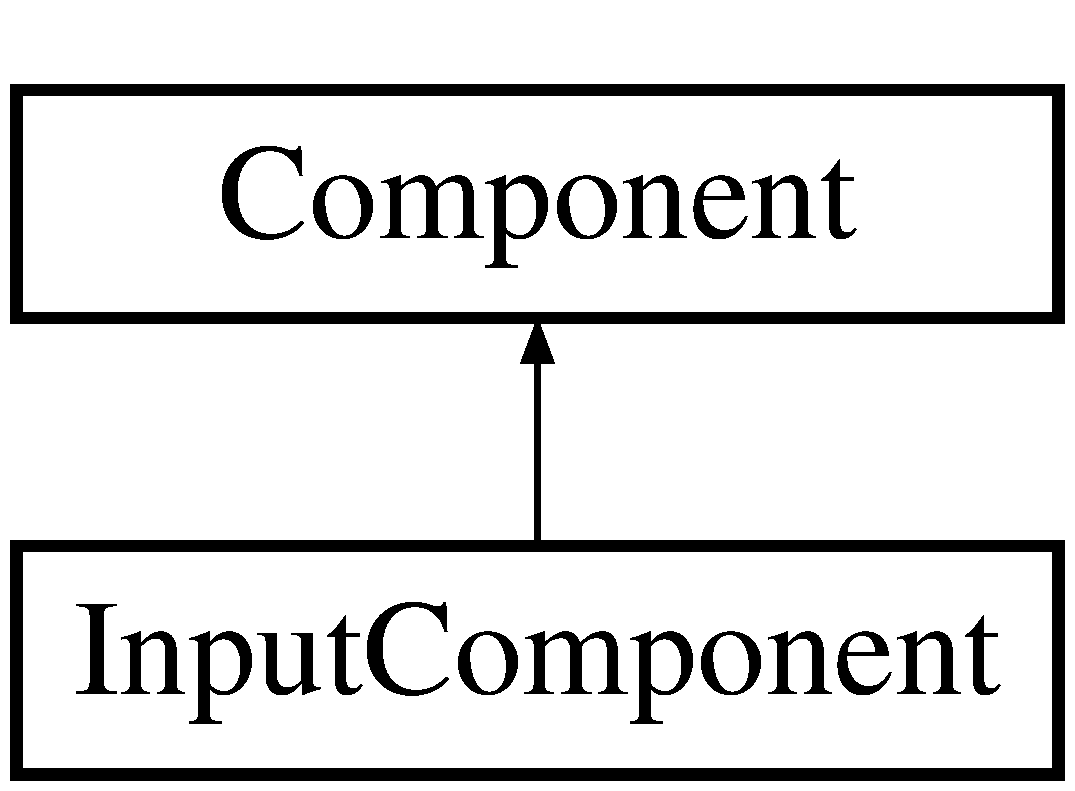
\includegraphics[height=2.000000cm]{class_input_component}
\end{center}
\end{figure}
\subsection*{Public Member Functions}
\begin{DoxyCompactItemize}
\item 
\mbox{\hyperlink{class_input_component_ae3af150f66c8e72ea4bef4b089c48d99}{Input\+Component}} ()
\item 
\mbox{\hyperlink{class_input_component_a50e6b9501302f0c8f055325ca652050e}{$\sim$\+Input\+Component}} ()
\item 
void \mbox{\hyperlink{class_input_component_ad4262870839371f79747db5b6faf25a7}{Initialize\+Component}} ()
\item 
void \mbox{\hyperlink{class_input_component_a99f431a305362899b8a6682b390c8899}{Pre\+Update}} ()
\item 
void \mbox{\hyperlink{class_input_component_a42d3b0dffbedfd8cf62702096780ed4d}{Update\+Component}} (float delta\+Time)
\end{DoxyCompactItemize}
\subsection*{Public Attributes}
\begin{DoxyCompactItemize}
\item 
std\+::unique\+\_\+ptr$<$ \mbox{\hyperlink{class_gamepad}{Gamepad}} $>$ \mbox{\hyperlink{class_input_component_a73abf6fc0132814d3cdca33aa5d3dfba}{m\+\_\+gamepad}}
\end{DoxyCompactItemize}
\subsection*{Additional Inherited Members}


\subsection{Detailed Description}
Input component. 

\subsection{Constructor \& Destructor Documentation}
\mbox{\Hypertarget{class_input_component_ae3af150f66c8e72ea4bef4b089c48d99}\label{class_input_component_ae3af150f66c8e72ea4bef4b089c48d99}} 
\index{Input\+Component@{Input\+Component}!Input\+Component@{Input\+Component}}
\index{Input\+Component@{Input\+Component}!Input\+Component@{Input\+Component}}
\subsubsection{\texorpdfstring{Input\+Component()}{InputComponent()}}
{\footnotesize\ttfamily Input\+Component\+::\+Input\+Component (\begin{DoxyParamCaption}{ }\end{DoxyParamCaption})}

Default constructor. \mbox{\Hypertarget{class_input_component_a50e6b9501302f0c8f055325ca652050e}\label{class_input_component_a50e6b9501302f0c8f055325ca652050e}} 
\index{Input\+Component@{Input\+Component}!````~Input\+Component@{$\sim$\+Input\+Component}}
\index{````~Input\+Component@{$\sim$\+Input\+Component}!Input\+Component@{Input\+Component}}
\subsubsection{\texorpdfstring{$\sim$\+Input\+Component()}{~InputComponent()}}
{\footnotesize\ttfamily Input\+Component\+::$\sim$\+Input\+Component (\begin{DoxyParamCaption}{ }\end{DoxyParamCaption})}

Default destructor. 

\subsection{Member Function Documentation}
\mbox{\Hypertarget{class_input_component_ad4262870839371f79747db5b6faf25a7}\label{class_input_component_ad4262870839371f79747db5b6faf25a7}} 
\index{Input\+Component@{Input\+Component}!Initialize\+Component@{Initialize\+Component}}
\index{Initialize\+Component@{Initialize\+Component}!Input\+Component@{Input\+Component}}
\subsubsection{\texorpdfstring{Initialize\+Component()}{InitializeComponent()}}
{\footnotesize\ttfamily void Input\+Component\+::\+Initialize\+Component (\begin{DoxyParamCaption}{ }\end{DoxyParamCaption})\hspace{0.3cm}{\ttfamily [virtual]}}

Initialize this component. 

Reimplemented from \mbox{\hyperlink{class_component_a65053e7e92ff6344e6b028111e43c3c9}{Component}}.

\mbox{\Hypertarget{class_input_component_a99f431a305362899b8a6682b390c8899}\label{class_input_component_a99f431a305362899b8a6682b390c8899}} 
\index{Input\+Component@{Input\+Component}!Pre\+Update@{Pre\+Update}}
\index{Pre\+Update@{Pre\+Update}!Input\+Component@{Input\+Component}}
\subsubsection{\texorpdfstring{Pre\+Update()}{PreUpdate()}}
{\footnotesize\ttfamily void Input\+Component\+::\+Pre\+Update (\begin{DoxyParamCaption}{ }\end{DoxyParamCaption})\hspace{0.3cm}{\ttfamily [virtual]}}

Called before the main update function. 

Reimplemented from \mbox{\hyperlink{class_component_a7866088cbcf6713821951955eadc85ce}{Component}}.

\mbox{\Hypertarget{class_input_component_a42d3b0dffbedfd8cf62702096780ed4d}\label{class_input_component_a42d3b0dffbedfd8cf62702096780ed4d}} 
\index{Input\+Component@{Input\+Component}!Update\+Component@{Update\+Component}}
\index{Update\+Component@{Update\+Component}!Input\+Component@{Input\+Component}}
\subsubsection{\texorpdfstring{Update\+Component()}{UpdateComponent()}}
{\footnotesize\ttfamily void Input\+Component\+::\+Update\+Component (\begin{DoxyParamCaption}\item[{float}]{delta\+Time }\end{DoxyParamCaption})\hspace{0.3cm}{\ttfamily [virtual]}}

Update this component called, called once per frame. 

Reimplemented from \mbox{\hyperlink{class_component_a8afb7c9504f763728bfedf642cfc5f43}{Component}}.



\subsection{Member Data Documentation}
\mbox{\Hypertarget{class_input_component_a73abf6fc0132814d3cdca33aa5d3dfba}\label{class_input_component_a73abf6fc0132814d3cdca33aa5d3dfba}} 
\index{Input\+Component@{Input\+Component}!m\+\_\+gamepad@{m\+\_\+gamepad}}
\index{m\+\_\+gamepad@{m\+\_\+gamepad}!Input\+Component@{Input\+Component}}
\subsubsection{\texorpdfstring{m\+\_\+gamepad}{m\_gamepad}}
{\footnotesize\ttfamily std\+::unique\+\_\+ptr$<$\mbox{\hyperlink{class_gamepad}{Gamepad}}$>$ Input\+Component\+::m\+\_\+gamepad}

\mbox{\hyperlink{class_gamepad}{Gamepad}} object 

The documentation for this class was generated from the following files\+:\begin{DoxyCompactItemize}
\item 
Engine/\+Source/\+Runtime/\+Game\+Object/\+Components/\mbox{\hyperlink{_input_component_8h}{Input\+Component.\+h}}\item 
Engine/\+Source/\+Runtime/\+Game\+Object/\+Components/\mbox{\hyperlink{_input_component_8cpp}{Input\+Component.\+cpp}}\end{DoxyCompactItemize}

\hypertarget{class_lua_manager}{}\section{Lua\+Manager Class Reference}
\label{class_lua_manager}\index{Lua\+Manager@{Lua\+Manager}}


{\ttfamily \#include $<$Lua\+Manager.\+h$>$}

\subsection*{Public Member Functions}
\begin{DoxyCompactItemize}
\item 
\mbox{\hyperlink{class_lua_manager_a11da08140b20bfb4e77ac117a6bc7a0a}{Lua\+Manager}} ()
\item 
\mbox{\hyperlink{class_lua_manager_a26a821d05088bb1a6d7642b6312930aa}{$\sim$\+Lua\+Manager}} ()
\item 
void \mbox{\hyperlink{class_lua_manager_a839c0f1bea728a4aa055b8e0be26bc27}{Init}} ()
\item 
void \mbox{\hyperlink{class_lua_manager_aa03c69244e112bcd5377c8fe965a5136}{Exceute\+String}} (const std\+::string \&str)
\item 
void \mbox{\hyperlink{class_lua_manager_a5c770602033c62a3eba4ece231c33ed5}{Execute\+File}} (const std\+::string \&file\+Path)
\item 
sol\+::table \mbox{\hyperlink{class_lua_manager_af885a50a5fe0368b32853385342ae7e6}{Get\+Table\+Keys}} (const std\+::string \&name)
\item 
std\+::shared\+\_\+ptr$<$ \mbox{\hyperlink{class_entity}{Entity}} $>$ \mbox{\hyperlink{class_lua_manager_a04d24b48c0d51473d64a956fc800c312}{Load\+Entity}} (const std\+::string \&type)
\end{DoxyCompactItemize}


\subsection{Detailed Description}
High-\/level manager for managing lua script objects. 

\subsection{Constructor \& Destructor Documentation}
\mbox{\Hypertarget{class_lua_manager_a11da08140b20bfb4e77ac117a6bc7a0a}\label{class_lua_manager_a11da08140b20bfb4e77ac117a6bc7a0a}} 
\index{Lua\+Manager@{Lua\+Manager}!Lua\+Manager@{Lua\+Manager}}
\index{Lua\+Manager@{Lua\+Manager}!Lua\+Manager@{Lua\+Manager}}
\subsubsection{\texorpdfstring{Lua\+Manager()}{LuaManager()}}
{\footnotesize\ttfamily Lua\+Manager\+::\+Lua\+Manager (\begin{DoxyParamCaption}{ }\end{DoxyParamCaption})}

Default constructor. \mbox{\Hypertarget{class_lua_manager_a26a821d05088bb1a6d7642b6312930aa}\label{class_lua_manager_a26a821d05088bb1a6d7642b6312930aa}} 
\index{Lua\+Manager@{Lua\+Manager}!````~Lua\+Manager@{$\sim$\+Lua\+Manager}}
\index{````~Lua\+Manager@{$\sim$\+Lua\+Manager}!Lua\+Manager@{Lua\+Manager}}
\subsubsection{\texorpdfstring{$\sim$\+Lua\+Manager()}{~LuaManager()}}
{\footnotesize\ttfamily Lua\+Manager\+::$\sim$\+Lua\+Manager (\begin{DoxyParamCaption}{ }\end{DoxyParamCaption})}

Default destructor. 

\subsection{Member Function Documentation}
\mbox{\Hypertarget{class_lua_manager_aa03c69244e112bcd5377c8fe965a5136}\label{class_lua_manager_aa03c69244e112bcd5377c8fe965a5136}} 
\index{Lua\+Manager@{Lua\+Manager}!Exceute\+String@{Exceute\+String}}
\index{Exceute\+String@{Exceute\+String}!Lua\+Manager@{Lua\+Manager}}
\subsubsection{\texorpdfstring{Exceute\+String()}{ExceuteString()}}
{\footnotesize\ttfamily void Lua\+Manager\+::\+Exceute\+String (\begin{DoxyParamCaption}\item[{const std\+::string \&}]{str }\end{DoxyParamCaption})}

Load and execute a lua script from a string \mbox{\Hypertarget{class_lua_manager_a5c770602033c62a3eba4ece231c33ed5}\label{class_lua_manager_a5c770602033c62a3eba4ece231c33ed5}} 
\index{Lua\+Manager@{Lua\+Manager}!Execute\+File@{Execute\+File}}
\index{Execute\+File@{Execute\+File}!Lua\+Manager@{Lua\+Manager}}
\subsubsection{\texorpdfstring{Execute\+File()}{ExecuteFile()}}
{\footnotesize\ttfamily void Lua\+Manager\+::\+Execute\+File (\begin{DoxyParamCaption}\item[{const std\+::string \&}]{file\+Path }\end{DoxyParamCaption})}

Load and execute a lua script from a file. \mbox{\Hypertarget{class_lua_manager_af885a50a5fe0368b32853385342ae7e6}\label{class_lua_manager_af885a50a5fe0368b32853385342ae7e6}} 
\index{Lua\+Manager@{Lua\+Manager}!Get\+Table\+Keys@{Get\+Table\+Keys}}
\index{Get\+Table\+Keys@{Get\+Table\+Keys}!Lua\+Manager@{Lua\+Manager}}
\subsubsection{\texorpdfstring{Get\+Table\+Keys()}{GetTableKeys()}}
{\footnotesize\ttfamily sol\+::table Lua\+Manager\+::\+Get\+Table\+Keys (\begin{DoxyParamCaption}\item[{const std\+::string \&}]{name }\end{DoxyParamCaption})}

Retrieves table keys from a lua script. \mbox{\Hypertarget{class_lua_manager_a839c0f1bea728a4aa055b8e0be26bc27}\label{class_lua_manager_a839c0f1bea728a4aa055b8e0be26bc27}} 
\index{Lua\+Manager@{Lua\+Manager}!Init@{Init}}
\index{Init@{Init}!Lua\+Manager@{Lua\+Manager}}
\subsubsection{\texorpdfstring{Init()}{Init()}}
{\footnotesize\ttfamily void Lua\+Manager\+::\+Init (\begin{DoxyParamCaption}{ }\end{DoxyParamCaption})}

Initializes the lua state manager object. \mbox{\Hypertarget{class_lua_manager_a04d24b48c0d51473d64a956fc800c312}\label{class_lua_manager_a04d24b48c0d51473d64a956fc800c312}} 
\index{Lua\+Manager@{Lua\+Manager}!Load\+Entity@{Load\+Entity}}
\index{Load\+Entity@{Load\+Entity}!Lua\+Manager@{Lua\+Manager}}
\subsubsection{\texorpdfstring{Load\+Entity()}{LoadEntity()}}
{\footnotesize\ttfamily std\+::shared\+\_\+ptr$<$ \mbox{\hyperlink{class_entity}{Entity}} $>$ Lua\+Manager\+::\+Load\+Entity (\begin{DoxyParamCaption}\item[{const std\+::string \&}]{type }\end{DoxyParamCaption})}

Load an entity from a lua script file. 

The documentation for this class was generated from the following files\+:\begin{DoxyCompactItemize}
\item 
Engine/\+Source/\+Runtime/\+Scripting\+System/\mbox{\hyperlink{_lua_manager_8h}{Lua\+Manager.\+h}}\item 
Engine/\+Source/\+Runtime/\+Scripting\+System/\mbox{\hyperlink{_lua_manager_8cpp}{Lua\+Manager.\+cpp}}\end{DoxyCompactItemize}

\hypertarget{class_math}{}\section{Math Class Reference}
\label{class_math}\index{Math@{Math}}


{\ttfamily \#include $<$Math.\+h$>$}



The documentation for this class was generated from the following file\+:\begin{DoxyCompactItemize}
\item 
Engine/\+Source/\+Runtime/\+Math/\mbox{\hyperlink{_math_8h}{Math.\+h}}\end{DoxyCompactItemize}

\hypertarget{class_memory_allocator}{}\section{Memory\+Allocator Class Reference}
\label{class_memory_allocator}\index{Memory\+Allocator@{Memory\+Allocator}}


{\ttfamily \#include $<$Memory\+Allocator.\+h$>$}

\subsection*{Public Member Functions}
\begin{DoxyCompactItemize}
\item 
\mbox{\hyperlink{class_memory_allocator_aeb408be3b4170052a477bd917bfba8a4}{Memory\+Allocator}} ()
\item 
\mbox{\hyperlink{class_memory_allocator_ad1f08b45facfce42c5103f726eb4e6d5}{Memory\+Allocator}} (size\+\_\+t size, void $\ast$ptr)
\item 
\mbox{\hyperlink{class_memory_allocator_a29649a1c897a6edca2a223ee9a100f34}{$\sim$\+Memory\+Allocator}} ()
\item 
virtual void $\ast$ \mbox{\hyperlink{class_memory_allocator_aa56c860aa8027554aa9bd6d7c9780a67}{Allocate}} (size\+\_\+t $\ast$size, uint8\+\_\+t alignment)=0
\item 
virtual void \mbox{\hyperlink{class_memory_allocator_ae6ee38cd52e3e0710251b4e3eb550c6d}{Free}} (void $\ast$ptr)=0
\item 
virtual void \mbox{\hyperlink{class_memory_allocator_a204e81d93d93f1db39e134b956422e56}{Clear}} ()=0
\end{DoxyCompactItemize}
\subsection*{Protected Attributes}
\begin{DoxyCompactItemize}
\item 
void $\ast$ \mbox{\hyperlink{class_memory_allocator_a62ec2c2ef91d62f61e630c75844b1279}{m\+\_\+first\+Memory\+Address}}
\item 
size\+\_\+t \mbox{\hyperlink{class_memory_allocator_a219f6c1d24a8a556f4d1ec1bb0b11171}{m\+\_\+memory\+Size}}
\item 
size\+\_\+t \mbox{\hyperlink{class_memory_allocator_a5961e1f05827593c67b17094ff8007bf}{m\+\_\+memory\+Used}}
\item 
uint64\+\_\+t \mbox{\hyperlink{class_memory_allocator_a0fbd7580dfb92e7e5ba20c44658df574}{m\+\_\+num\+Memory\+Allocations}}
\end{DoxyCompactItemize}


\subsection{Detailed Description}
Base memory allocator class. 

\subsection{Constructor \& Destructor Documentation}
\mbox{\Hypertarget{class_memory_allocator_aeb408be3b4170052a477bd917bfba8a4}\label{class_memory_allocator_aeb408be3b4170052a477bd917bfba8a4}} 
\index{Memory\+Allocator@{Memory\+Allocator}!Memory\+Allocator@{Memory\+Allocator}}
\index{Memory\+Allocator@{Memory\+Allocator}!Memory\+Allocator@{Memory\+Allocator}}
\subsubsection{\texorpdfstring{Memory\+Allocator()}{MemoryAllocator()}\hspace{0.1cm}{\footnotesize\ttfamily [1/2]}}
{\footnotesize\ttfamily Memory\+Allocator\+::\+Memory\+Allocator (\begin{DoxyParamCaption}{ }\end{DoxyParamCaption})}

Default constructor. \mbox{\Hypertarget{class_memory_allocator_ad1f08b45facfce42c5103f726eb4e6d5}\label{class_memory_allocator_ad1f08b45facfce42c5103f726eb4e6d5}} 
\index{Memory\+Allocator@{Memory\+Allocator}!Memory\+Allocator@{Memory\+Allocator}}
\index{Memory\+Allocator@{Memory\+Allocator}!Memory\+Allocator@{Memory\+Allocator}}
\subsubsection{\texorpdfstring{Memory\+Allocator()}{MemoryAllocator()}\hspace{0.1cm}{\footnotesize\ttfamily [2/2]}}
{\footnotesize\ttfamily Memory\+Allocator\+::\+Memory\+Allocator (\begin{DoxyParamCaption}\item[{size\+\_\+t}]{size,  }\item[{void $\ast$}]{ptr }\end{DoxyParamCaption})}

Constructor. \mbox{\Hypertarget{class_memory_allocator_a29649a1c897a6edca2a223ee9a100f34}\label{class_memory_allocator_a29649a1c897a6edca2a223ee9a100f34}} 
\index{Memory\+Allocator@{Memory\+Allocator}!````~Memory\+Allocator@{$\sim$\+Memory\+Allocator}}
\index{````~Memory\+Allocator@{$\sim$\+Memory\+Allocator}!Memory\+Allocator@{Memory\+Allocator}}
\subsubsection{\texorpdfstring{$\sim$\+Memory\+Allocator()}{~MemoryAllocator()}}
{\footnotesize\ttfamily Memory\+Allocator\+::$\sim$\+Memory\+Allocator (\begin{DoxyParamCaption}{ }\end{DoxyParamCaption})}

Default destructor. 

\subsection{Member Function Documentation}
\mbox{\Hypertarget{class_memory_allocator_aa56c860aa8027554aa9bd6d7c9780a67}\label{class_memory_allocator_aa56c860aa8027554aa9bd6d7c9780a67}} 
\index{Memory\+Allocator@{Memory\+Allocator}!Allocate@{Allocate}}
\index{Allocate@{Allocate}!Memory\+Allocator@{Memory\+Allocator}}
\subsubsection{\texorpdfstring{Allocate()}{Allocate()}}
{\footnotesize\ttfamily virtual void$\ast$ Memory\+Allocator\+::\+Allocate (\begin{DoxyParamCaption}\item[{size\+\_\+t $\ast$}]{size,  }\item[{uint8\+\_\+t}]{alignment }\end{DoxyParamCaption})\hspace{0.3cm}{\ttfamily [pure virtual]}}

Allocate memory. \mbox{\Hypertarget{class_memory_allocator_a204e81d93d93f1db39e134b956422e56}\label{class_memory_allocator_a204e81d93d93f1db39e134b956422e56}} 
\index{Memory\+Allocator@{Memory\+Allocator}!Clear@{Clear}}
\index{Clear@{Clear}!Memory\+Allocator@{Memory\+Allocator}}
\subsubsection{\texorpdfstring{Clear()}{Clear()}}
{\footnotesize\ttfamily virtual void Memory\+Allocator\+::\+Clear (\begin{DoxyParamCaption}{ }\end{DoxyParamCaption})\hspace{0.3cm}{\ttfamily [pure virtual]}}

Clear all allocated memory. \mbox{\Hypertarget{class_memory_allocator_ae6ee38cd52e3e0710251b4e3eb550c6d}\label{class_memory_allocator_ae6ee38cd52e3e0710251b4e3eb550c6d}} 
\index{Memory\+Allocator@{Memory\+Allocator}!Free@{Free}}
\index{Free@{Free}!Memory\+Allocator@{Memory\+Allocator}}
\subsubsection{\texorpdfstring{Free()}{Free()}}
{\footnotesize\ttfamily virtual void Memory\+Allocator\+::\+Free (\begin{DoxyParamCaption}\item[{void $\ast$}]{ptr }\end{DoxyParamCaption})\hspace{0.3cm}{\ttfamily [pure virtual]}}

Free a specifically allocated memory address. 

\subsection{Member Data Documentation}
\mbox{\Hypertarget{class_memory_allocator_a62ec2c2ef91d62f61e630c75844b1279}\label{class_memory_allocator_a62ec2c2ef91d62f61e630c75844b1279}} 
\index{Memory\+Allocator@{Memory\+Allocator}!m\+\_\+first\+Memory\+Address@{m\+\_\+first\+Memory\+Address}}
\index{m\+\_\+first\+Memory\+Address@{m\+\_\+first\+Memory\+Address}!Memory\+Allocator@{Memory\+Allocator}}
\subsubsection{\texorpdfstring{m\+\_\+first\+Memory\+Address}{m\_firstMemoryAddress}}
{\footnotesize\ttfamily void$\ast$ Memory\+Allocator\+::m\+\_\+first\+Memory\+Address\hspace{0.3cm}{\ttfamily [protected]}}

Pointer to the first memory address. \mbox{\Hypertarget{class_memory_allocator_a219f6c1d24a8a556f4d1ec1bb0b11171}\label{class_memory_allocator_a219f6c1d24a8a556f4d1ec1bb0b11171}} 
\index{Memory\+Allocator@{Memory\+Allocator}!m\+\_\+memory\+Size@{m\+\_\+memory\+Size}}
\index{m\+\_\+memory\+Size@{m\+\_\+memory\+Size}!Memory\+Allocator@{Memory\+Allocator}}
\subsubsection{\texorpdfstring{m\+\_\+memory\+Size}{m\_memorySize}}
{\footnotesize\ttfamily size\+\_\+t Memory\+Allocator\+::m\+\_\+memory\+Size\hspace{0.3cm}{\ttfamily [protected]}}

Size of the memory in bytes. \mbox{\Hypertarget{class_memory_allocator_a5961e1f05827593c67b17094ff8007bf}\label{class_memory_allocator_a5961e1f05827593c67b17094ff8007bf}} 
\index{Memory\+Allocator@{Memory\+Allocator}!m\+\_\+memory\+Used@{m\+\_\+memory\+Used}}
\index{m\+\_\+memory\+Used@{m\+\_\+memory\+Used}!Memory\+Allocator@{Memory\+Allocator}}
\subsubsection{\texorpdfstring{m\+\_\+memory\+Used}{m\_memoryUsed}}
{\footnotesize\ttfamily size\+\_\+t Memory\+Allocator\+::m\+\_\+memory\+Used\hspace{0.3cm}{\ttfamily [protected]}}

Size of the memory used in bytes. \mbox{\Hypertarget{class_memory_allocator_a0fbd7580dfb92e7e5ba20c44658df574}\label{class_memory_allocator_a0fbd7580dfb92e7e5ba20c44658df574}} 
\index{Memory\+Allocator@{Memory\+Allocator}!m\+\_\+num\+Memory\+Allocations@{m\+\_\+num\+Memory\+Allocations}}
\index{m\+\_\+num\+Memory\+Allocations@{m\+\_\+num\+Memory\+Allocations}!Memory\+Allocator@{Memory\+Allocator}}
\subsubsection{\texorpdfstring{m\+\_\+num\+Memory\+Allocations}{m\_numMemoryAllocations}}
{\footnotesize\ttfamily uint64\+\_\+t Memory\+Allocator\+::m\+\_\+num\+Memory\+Allocations\hspace{0.3cm}{\ttfamily [protected]}}

Number of memory allocations. 

The documentation for this class was generated from the following files\+:\begin{DoxyCompactItemize}
\item 
Engine/\+Source/\+Runtime/\+Memory/\mbox{\hyperlink{_memory_allocator_8h}{Memory\+Allocator.\+h}}\item 
Engine/\+Source/\+Runtime/\+Memory/\mbox{\hyperlink{_memory_allocator_8cpp}{Memory\+Allocator.\+cpp}}\end{DoxyCompactItemize}

\hypertarget{class_renderer}{}\section{Renderer Class Reference}
\label{class_renderer}\index{Renderer@{Renderer}}


{\ttfamily \#include $<$Renderer.\+h$>$}

\subsection*{Public Member Functions}
\begin{DoxyCompactItemize}
\item 
\mbox{\hyperlink{class_renderer_a7ebf46f54dab9905f79b80f7fddb76a6}{Renderer}} ()
\item 
\mbox{\hyperlink{class_renderer_afeee408862d5bd6255a6882d47e6d5cd}{$\sim$\+Renderer}} ()
\item 
void \mbox{\hyperlink{class_renderer_aa3d40d03451dab486e098b8f337c0f87}{Initialize}} (S\+D\+L\+\_\+\+Window $\ast$window)
\item 
void \mbox{\hyperlink{class_renderer_aeedbc2ffdccf51fa1384100446488746}{Clear}} ()
\item 
void \mbox{\hyperlink{class_renderer_a09f2d3c7bac8ff314d860b9958a8531c}{Swap\+Buffers}} ()
\item 
S\+D\+L\+\_\+\+Renderer $\ast$ \mbox{\hyperlink{class_renderer_a10f0554599d4fde891984d41d0e45c05}{Get\+S\+D\+L\+Renderer}} () const
\end{DoxyCompactItemize}


\subsection{Detailed Description}
Abstraction layer for the S\+DL renderer. 

\subsection{Constructor \& Destructor Documentation}
\mbox{\Hypertarget{class_renderer_a7ebf46f54dab9905f79b80f7fddb76a6}\label{class_renderer_a7ebf46f54dab9905f79b80f7fddb76a6}} 
\index{Renderer@{Renderer}!Renderer@{Renderer}}
\index{Renderer@{Renderer}!Renderer@{Renderer}}
\subsubsection{\texorpdfstring{Renderer()}{Renderer()}}
{\footnotesize\ttfamily Renderer\+::\+Renderer (\begin{DoxyParamCaption}{ }\end{DoxyParamCaption})}

Default constructor. \mbox{\Hypertarget{class_renderer_afeee408862d5bd6255a6882d47e6d5cd}\label{class_renderer_afeee408862d5bd6255a6882d47e6d5cd}} 
\index{Renderer@{Renderer}!````~Renderer@{$\sim$\+Renderer}}
\index{````~Renderer@{$\sim$\+Renderer}!Renderer@{Renderer}}
\subsubsection{\texorpdfstring{$\sim$\+Renderer()}{~Renderer()}}
{\footnotesize\ttfamily Renderer\+::$\sim$\+Renderer (\begin{DoxyParamCaption}{ }\end{DoxyParamCaption})}

Default destructor. 

\subsection{Member Function Documentation}
\mbox{\Hypertarget{class_renderer_aeedbc2ffdccf51fa1384100446488746}\label{class_renderer_aeedbc2ffdccf51fa1384100446488746}} 
\index{Renderer@{Renderer}!Clear@{Clear}}
\index{Clear@{Clear}!Renderer@{Renderer}}
\subsubsection{\texorpdfstring{Clear()}{Clear()}}
{\footnotesize\ttfamily void Renderer\+::\+Clear (\begin{DoxyParamCaption}{ }\end{DoxyParamCaption})}

Clear buffer. \mbox{\Hypertarget{class_renderer_a10f0554599d4fde891984d41d0e45c05}\label{class_renderer_a10f0554599d4fde891984d41d0e45c05}} 
\index{Renderer@{Renderer}!Get\+S\+D\+L\+Renderer@{Get\+S\+D\+L\+Renderer}}
\index{Get\+S\+D\+L\+Renderer@{Get\+S\+D\+L\+Renderer}!Renderer@{Renderer}}
\subsubsection{\texorpdfstring{Get\+S\+D\+L\+Renderer()}{GetSDLRenderer()}}
{\footnotesize\ttfamily S\+D\+L\+\_\+\+Renderer$\ast$ Renderer\+::\+Get\+S\+D\+L\+Renderer (\begin{DoxyParamCaption}{ }\end{DoxyParamCaption}) const\hspace{0.3cm}{\ttfamily [inline]}}

Retunrs a pointer to the S\+DL renderer. \mbox{\Hypertarget{class_renderer_aa3d40d03451dab486e098b8f337c0f87}\label{class_renderer_aa3d40d03451dab486e098b8f337c0f87}} 
\index{Renderer@{Renderer}!Initialize@{Initialize}}
\index{Initialize@{Initialize}!Renderer@{Renderer}}
\subsubsection{\texorpdfstring{Initialize()}{Initialize()}}
{\footnotesize\ttfamily void Renderer\+::\+Initialize (\begin{DoxyParamCaption}\item[{S\+D\+L\+\_\+\+Window $\ast$}]{window }\end{DoxyParamCaption})}

Initialize the renderer object. \mbox{\Hypertarget{class_renderer_a09f2d3c7bac8ff314d860b9958a8531c}\label{class_renderer_a09f2d3c7bac8ff314d860b9958a8531c}} 
\index{Renderer@{Renderer}!Swap\+Buffers@{Swap\+Buffers}}
\index{Swap\+Buffers@{Swap\+Buffers}!Renderer@{Renderer}}
\subsubsection{\texorpdfstring{Swap\+Buffers()}{SwapBuffers()}}
{\footnotesize\ttfamily void Renderer\+::\+Swap\+Buffers (\begin{DoxyParamCaption}{ }\end{DoxyParamCaption})}

Swap buffer 

The documentation for this class was generated from the following files\+:\begin{DoxyCompactItemize}
\item 
Engine/\+Source/\+Runtime/\+Core/\mbox{\hyperlink{_renderer_8h}{Renderer.\+h}}\item 
Engine/\+Source/\+Runtime/\+Core/\mbox{\hyperlink{_renderer_8cpp}{Renderer.\+cpp}}\end{DoxyCompactItemize}

\hypertarget{class_singleton_object}{}\section{Singleton\+Object$<$ T $>$ Class Template Reference}
\label{class_singleton_object}\index{Singleton\+Object$<$ T $>$@{Singleton\+Object$<$ T $>$}}


{\ttfamily \#include $<$Singleton\+Object.\+h$>$}

\subsection*{Public Member Functions}
\begin{DoxyCompactItemize}
\item 
\mbox{\hyperlink{class_singleton_object_aed804192a73e9d8b935d9cbc6c817877}{Singleton\+Object}} ()
\item 
virtual \mbox{\hyperlink{class_singleton_object_ae8fbe0c316c1927836efd6c2712b892d}{$\sim$\+Singleton\+Object}} ()
\end{DoxyCompactItemize}
\subsection*{Static Public Member Functions}
\begin{DoxyCompactItemize}
\item 
static T \& \mbox{\hyperlink{class_singleton_object_adabe7b9f1b8ed85ec9a2e2b4a6d29aac}{Get\+Object\+Reference}} ()
\item 
static T $\ast$ \mbox{\hyperlink{class_singleton_object_aab1f7ff4e122cf6fc49217b620d55fd8}{Get\+Object}} ()
\end{DoxyCompactItemize}


\subsection{Detailed Description}
\subsubsection*{template$<$class T$>$\newline
class Singleton\+Object$<$ T $>$}

Enables the creation of a singleton object by creating a static global instance. 

\subsection{Constructor \& Destructor Documentation}
\mbox{\Hypertarget{class_singleton_object_aed804192a73e9d8b935d9cbc6c817877}\label{class_singleton_object_aed804192a73e9d8b935d9cbc6c817877}} 
\index{Singleton\+Object@{Singleton\+Object}!Singleton\+Object@{Singleton\+Object}}
\index{Singleton\+Object@{Singleton\+Object}!Singleton\+Object@{Singleton\+Object}}
\subsubsection{\texorpdfstring{Singleton\+Object()}{SingletonObject()}}
{\footnotesize\ttfamily template$<$class T$>$ \\
\mbox{\hyperlink{class_singleton_object}{Singleton\+Object}}$<$ T $>$\+::\mbox{\hyperlink{class_singleton_object}{Singleton\+Object}} (\begin{DoxyParamCaption}{ }\end{DoxyParamCaption})\hspace{0.3cm}{\ttfamily [inline]}}

Default constructor. \mbox{\Hypertarget{class_singleton_object_ae8fbe0c316c1927836efd6c2712b892d}\label{class_singleton_object_ae8fbe0c316c1927836efd6c2712b892d}} 
\index{Singleton\+Object@{Singleton\+Object}!````~Singleton\+Object@{$\sim$\+Singleton\+Object}}
\index{````~Singleton\+Object@{$\sim$\+Singleton\+Object}!Singleton\+Object@{Singleton\+Object}}
\subsubsection{\texorpdfstring{$\sim$\+Singleton\+Object()}{~SingletonObject()}}
{\footnotesize\ttfamily template$<$class T$>$ \\
virtual \mbox{\hyperlink{class_singleton_object}{Singleton\+Object}}$<$ T $>$\+::$\sim$\mbox{\hyperlink{class_singleton_object}{Singleton\+Object}} (\begin{DoxyParamCaption}{ }\end{DoxyParamCaption})\hspace{0.3cm}{\ttfamily [inline]}, {\ttfamily [virtual]}}

Default destructor. 

\subsection{Member Function Documentation}
\mbox{\Hypertarget{class_singleton_object_aab1f7ff4e122cf6fc49217b620d55fd8}\label{class_singleton_object_aab1f7ff4e122cf6fc49217b620d55fd8}} 
\index{Singleton\+Object@{Singleton\+Object}!Get\+Object@{Get\+Object}}
\index{Get\+Object@{Get\+Object}!Singleton\+Object@{Singleton\+Object}}
\subsubsection{\texorpdfstring{Get\+Object()}{GetObject()}}
{\footnotesize\ttfamily template$<$class T$>$ \\
static T$\ast$ \mbox{\hyperlink{class_singleton_object}{Singleton\+Object}}$<$ T $>$\+::Get\+Object (\begin{DoxyParamCaption}{ }\end{DoxyParamCaption})\hspace{0.3cm}{\ttfamily [inline]}, {\ttfamily [static]}}

Returns the singleton object. \mbox{\Hypertarget{class_singleton_object_adabe7b9f1b8ed85ec9a2e2b4a6d29aac}\label{class_singleton_object_adabe7b9f1b8ed85ec9a2e2b4a6d29aac}} 
\index{Singleton\+Object@{Singleton\+Object}!Get\+Object\+Reference@{Get\+Object\+Reference}}
\index{Get\+Object\+Reference@{Get\+Object\+Reference}!Singleton\+Object@{Singleton\+Object}}
\subsubsection{\texorpdfstring{Get\+Object\+Reference()}{GetObjectReference()}}
{\footnotesize\ttfamily template$<$class T$>$ \\
static T\& \mbox{\hyperlink{class_singleton_object}{Singleton\+Object}}$<$ T $>$\+::Get\+Object\+Reference (\begin{DoxyParamCaption}{ }\end{DoxyParamCaption})\hspace{0.3cm}{\ttfamily [inline]}, {\ttfamily [static]}}

Returns a reference to the singleton object. 

The documentation for this class was generated from the following file\+:\begin{DoxyCompactItemize}
\item 
Engine/\+Source/\+Runtime/\+Game\+Object/\mbox{\hyperlink{_singleton_object_8h}{Singleton\+Object.\+h}}\end{DoxyCompactItemize}

\hypertarget{class_sprite_component}{}\section{Sprite\+Component Class Reference}
\label{class_sprite_component}\index{Sprite\+Component@{Sprite\+Component}}


{\ttfamily \#include $<$Sprite\+Component.\+h$>$}

Inheritance diagram for Sprite\+Component\+:\begin{figure}[H]
\begin{center}
\leavevmode
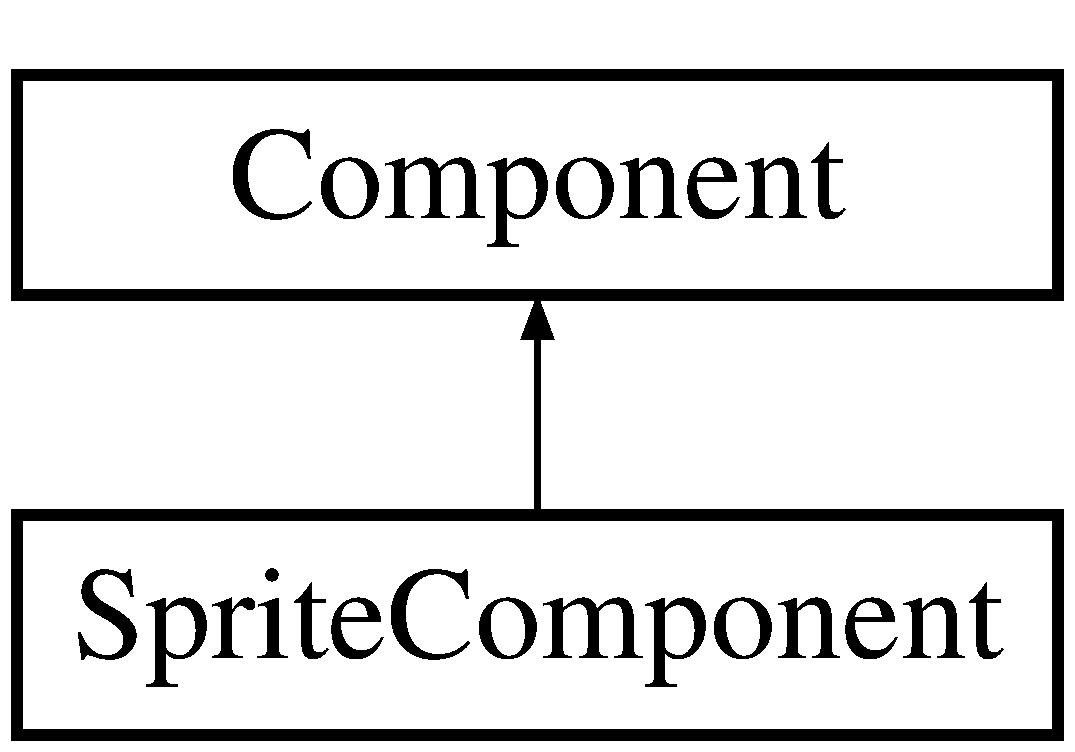
\includegraphics[height=2.000000cm]{class_sprite_component}
\end{center}
\end{figure}
\subsection*{Public Member Functions}
\begin{DoxyCompactItemize}
\item 
\mbox{\hyperlink{class_sprite_component_a5d7580c546b06d25e480ae7a20084120}{Sprite\+Component}} (S\+D\+L\+\_\+\+Renderer $\ast$renderer)
\item 
\mbox{\hyperlink{class_sprite_component_add14acc8523a724c112e6c93b750b60e}{$\sim$\+Sprite\+Component}} ()
\item 
void \mbox{\hyperlink{class_sprite_component_af4040c615bebb4aea20f274f77e36733}{Initialize\+Component}} () override
\item 
void \mbox{\hyperlink{class_sprite_component_aba00f9c0ecc0a0de41f271267c5440ff}{Update\+Component}} (float delta\+Time) override
\item 
void \mbox{\hyperlink{class_sprite_component_a429074e2f4eb31f92dff67fe1b89da55}{Set\+Filename}} (const std\+::string \&filepath)
\item 
void \mbox{\hyperlink{class_sprite_component_af71d7595507094e09d415cfa50e53fc3}{Create\+Texture}} (const std\+::string \&texture\+Path)
\item 
void \mbox{\hyperlink{class_sprite_component_ac696d85039713b2afbf4db0b361177b1}{Draw}} (S\+D\+L\+\_\+\+Renderer $\ast$renderer)
\item 
int32\+\_\+t \mbox{\hyperlink{class_sprite_component_aab677bb3904863fafcfaa4cb4790dd2a}{Get\+Sprite\+Draw\+Order}} () const
\item 
int32\+\_\+t \mbox{\hyperlink{class_sprite_component_a38889ac972abef595e94afe588a0f5f1}{Get\+Sprite\+Width}} () const
\item 
int32\+\_\+t \mbox{\hyperlink{class_sprite_component_a7a060e8695f35c136a78731b3d865f6e}{Get\+Sprite\+Height}} () const
\item 
std\+::string \mbox{\hyperlink{class_sprite_component_a20d83f167d220ec3b653bcd31262d6d7}{Get\+Sprite\+Name}} () const
\end{DoxyCompactItemize}
\subsection*{Additional Inherited Members}


\subsection{Constructor \& Destructor Documentation}
\mbox{\Hypertarget{class_sprite_component_a5d7580c546b06d25e480ae7a20084120}\label{class_sprite_component_a5d7580c546b06d25e480ae7a20084120}} 
\index{Sprite\+Component@{Sprite\+Component}!Sprite\+Component@{Sprite\+Component}}
\index{Sprite\+Component@{Sprite\+Component}!Sprite\+Component@{Sprite\+Component}}
\subsubsection{\texorpdfstring{Sprite\+Component()}{SpriteComponent()}}
{\footnotesize\ttfamily Sprite\+Component\+::\+Sprite\+Component (\begin{DoxyParamCaption}\item[{S\+D\+L\+\_\+\+Renderer $\ast$}]{renderer }\end{DoxyParamCaption})}

Constructor. \mbox{\Hypertarget{class_sprite_component_add14acc8523a724c112e6c93b750b60e}\label{class_sprite_component_add14acc8523a724c112e6c93b750b60e}} 
\index{Sprite\+Component@{Sprite\+Component}!````~Sprite\+Component@{$\sim$\+Sprite\+Component}}
\index{````~Sprite\+Component@{$\sim$\+Sprite\+Component}!Sprite\+Component@{Sprite\+Component}}
\subsubsection{\texorpdfstring{$\sim$\+Sprite\+Component()}{~SpriteComponent()}}
{\footnotesize\ttfamily Sprite\+Component\+::$\sim$\+Sprite\+Component (\begin{DoxyParamCaption}{ }\end{DoxyParamCaption})}

Default destructor. 

\subsection{Member Function Documentation}
\mbox{\Hypertarget{class_sprite_component_af71d7595507094e09d415cfa50e53fc3}\label{class_sprite_component_af71d7595507094e09d415cfa50e53fc3}} 
\index{Sprite\+Component@{Sprite\+Component}!Create\+Texture@{Create\+Texture}}
\index{Create\+Texture@{Create\+Texture}!Sprite\+Component@{Sprite\+Component}}
\subsubsection{\texorpdfstring{Create\+Texture()}{CreateTexture()}}
{\footnotesize\ttfamily void Sprite\+Component\+::\+Create\+Texture (\begin{DoxyParamCaption}\item[{const std\+::string \&}]{texture\+Path }\end{DoxyParamCaption})}

\mbox{\Hypertarget{class_sprite_component_ac696d85039713b2afbf4db0b361177b1}\label{class_sprite_component_ac696d85039713b2afbf4db0b361177b1}} 
\index{Sprite\+Component@{Sprite\+Component}!Draw@{Draw}}
\index{Draw@{Draw}!Sprite\+Component@{Sprite\+Component}}
\subsubsection{\texorpdfstring{Draw()}{Draw()}}
{\footnotesize\ttfamily void Sprite\+Component\+::\+Draw (\begin{DoxyParamCaption}\item[{S\+D\+L\+\_\+\+Renderer $\ast$}]{renderer }\end{DoxyParamCaption})}

\mbox{\Hypertarget{class_sprite_component_aab677bb3904863fafcfaa4cb4790dd2a}\label{class_sprite_component_aab677bb3904863fafcfaa4cb4790dd2a}} 
\index{Sprite\+Component@{Sprite\+Component}!Get\+Sprite\+Draw\+Order@{Get\+Sprite\+Draw\+Order}}
\index{Get\+Sprite\+Draw\+Order@{Get\+Sprite\+Draw\+Order}!Sprite\+Component@{Sprite\+Component}}
\subsubsection{\texorpdfstring{Get\+Sprite\+Draw\+Order()}{GetSpriteDrawOrder()}}
{\footnotesize\ttfamily int32\+\_\+t Sprite\+Component\+::\+Get\+Sprite\+Draw\+Order (\begin{DoxyParamCaption}{ }\end{DoxyParamCaption}) const\hspace{0.3cm}{\ttfamily [inline]}}

\mbox{\Hypertarget{class_sprite_component_a7a060e8695f35c136a78731b3d865f6e}\label{class_sprite_component_a7a060e8695f35c136a78731b3d865f6e}} 
\index{Sprite\+Component@{Sprite\+Component}!Get\+Sprite\+Height@{Get\+Sprite\+Height}}
\index{Get\+Sprite\+Height@{Get\+Sprite\+Height}!Sprite\+Component@{Sprite\+Component}}
\subsubsection{\texorpdfstring{Get\+Sprite\+Height()}{GetSpriteHeight()}}
{\footnotesize\ttfamily int32\+\_\+t Sprite\+Component\+::\+Get\+Sprite\+Height (\begin{DoxyParamCaption}{ }\end{DoxyParamCaption}) const\hspace{0.3cm}{\ttfamily [inline]}}

\mbox{\Hypertarget{class_sprite_component_a20d83f167d220ec3b653bcd31262d6d7}\label{class_sprite_component_a20d83f167d220ec3b653bcd31262d6d7}} 
\index{Sprite\+Component@{Sprite\+Component}!Get\+Sprite\+Name@{Get\+Sprite\+Name}}
\index{Get\+Sprite\+Name@{Get\+Sprite\+Name}!Sprite\+Component@{Sprite\+Component}}
\subsubsection{\texorpdfstring{Get\+Sprite\+Name()}{GetSpriteName()}}
{\footnotesize\ttfamily std\+::string Sprite\+Component\+::\+Get\+Sprite\+Name (\begin{DoxyParamCaption}{ }\end{DoxyParamCaption}) const\hspace{0.3cm}{\ttfamily [inline]}}

\mbox{\Hypertarget{class_sprite_component_a38889ac972abef595e94afe588a0f5f1}\label{class_sprite_component_a38889ac972abef595e94afe588a0f5f1}} 
\index{Sprite\+Component@{Sprite\+Component}!Get\+Sprite\+Width@{Get\+Sprite\+Width}}
\index{Get\+Sprite\+Width@{Get\+Sprite\+Width}!Sprite\+Component@{Sprite\+Component}}
\subsubsection{\texorpdfstring{Get\+Sprite\+Width()}{GetSpriteWidth()}}
{\footnotesize\ttfamily int32\+\_\+t Sprite\+Component\+::\+Get\+Sprite\+Width (\begin{DoxyParamCaption}{ }\end{DoxyParamCaption}) const\hspace{0.3cm}{\ttfamily [inline]}}

\mbox{\Hypertarget{class_sprite_component_af4040c615bebb4aea20f274f77e36733}\label{class_sprite_component_af4040c615bebb4aea20f274f77e36733}} 
\index{Sprite\+Component@{Sprite\+Component}!Initialize\+Component@{Initialize\+Component}}
\index{Initialize\+Component@{Initialize\+Component}!Sprite\+Component@{Sprite\+Component}}
\subsubsection{\texorpdfstring{Initialize\+Component()}{InitializeComponent()}}
{\footnotesize\ttfamily void Sprite\+Component\+::\+Initialize\+Component (\begin{DoxyParamCaption}{ }\end{DoxyParamCaption})\hspace{0.3cm}{\ttfamily [override]}, {\ttfamily [virtual]}}

Initialize this component. 

Reimplemented from \mbox{\hyperlink{class_component_a65053e7e92ff6344e6b028111e43c3c9}{Component}}.

\mbox{\Hypertarget{class_sprite_component_a429074e2f4eb31f92dff67fe1b89da55}\label{class_sprite_component_a429074e2f4eb31f92dff67fe1b89da55}} 
\index{Sprite\+Component@{Sprite\+Component}!Set\+Filename@{Set\+Filename}}
\index{Set\+Filename@{Set\+Filename}!Sprite\+Component@{Sprite\+Component}}
\subsubsection{\texorpdfstring{Set\+Filename()}{SetFilename()}}
{\footnotesize\ttfamily void Sprite\+Component\+::\+Set\+Filename (\begin{DoxyParamCaption}\item[{const std\+::string \&}]{filepath }\end{DoxyParamCaption})}

\mbox{\Hypertarget{class_sprite_component_aba00f9c0ecc0a0de41f271267c5440ff}\label{class_sprite_component_aba00f9c0ecc0a0de41f271267c5440ff}} 
\index{Sprite\+Component@{Sprite\+Component}!Update\+Component@{Update\+Component}}
\index{Update\+Component@{Update\+Component}!Sprite\+Component@{Sprite\+Component}}
\subsubsection{\texorpdfstring{Update\+Component()}{UpdateComponent()}}
{\footnotesize\ttfamily void Sprite\+Component\+::\+Update\+Component (\begin{DoxyParamCaption}\item[{float}]{delta\+Time }\end{DoxyParamCaption})\hspace{0.3cm}{\ttfamily [override]}, {\ttfamily [virtual]}}

Update this component, called once per frame. 

Reimplemented from \mbox{\hyperlink{class_component_a8afb7c9504f763728bfedf642cfc5f43}{Component}}.



The documentation for this class was generated from the following files\+:\begin{DoxyCompactItemize}
\item 
Engine/\+Source/\+Runtime/\+Game\+Object/\+Components/\mbox{\hyperlink{_sprite_component_8h}{Sprite\+Component.\+h}}\item 
Engine/\+Source/\+Runtime/\+Game\+Object/\+Components/\mbox{\hyperlink{_sprite_component_8cpp}{Sprite\+Component.\+cpp}}\end{DoxyCompactItemize}

\hypertarget{class_string}{}\section{String Class Reference}
\label{class_string}\index{String@{String}}


{\ttfamily \#include $<$String.\+h$>$}

\subsection*{Static Public Member Functions}
\begin{DoxyCompactItemize}
\item 
static std\+::string \mbox{\hyperlink{class_string_a30760cf947e41b306621aeb2da0a1eee}{Normalize}} (std\+::string \&str)
\end{DoxyCompactItemize}


\subsection{Detailed Description}
\mbox{\hyperlink{class_string}{String}} utility class. 

\subsection{Member Function Documentation}
\mbox{\Hypertarget{class_string_a30760cf947e41b306621aeb2da0a1eee}\label{class_string_a30760cf947e41b306621aeb2da0a1eee}} 
\index{String@{String}!Normalize@{Normalize}}
\index{Normalize@{Normalize}!String@{String}}
\subsubsection{\texorpdfstring{Normalize()}{Normalize()}}
{\footnotesize\ttfamily static std\+::string String\+::\+Normalize (\begin{DoxyParamCaption}\item[{std\+::string \&}]{str }\end{DoxyParamCaption})\hspace{0.3cm}{\ttfamily [inline]}, {\ttfamily [static]}}

Normalize a given string. 

The documentation for this class was generated from the following file\+:\begin{DoxyCompactItemize}
\item 
Engine/\+Source/\+Runtime/\+String/\mbox{\hyperlink{_string_8h}{String.\+h}}\end{DoxyCompactItemize}

\hypertarget{class_texture_asset}{}\section{Texture\+Asset Class Reference}
\label{class_texture_asset}\index{Texture\+Asset@{Texture\+Asset}}


{\ttfamily \#include $<$Texture\+Asset.\+h$>$}

Inheritance diagram for Texture\+Asset\+:\begin{figure}[H]
\begin{center}
\leavevmode
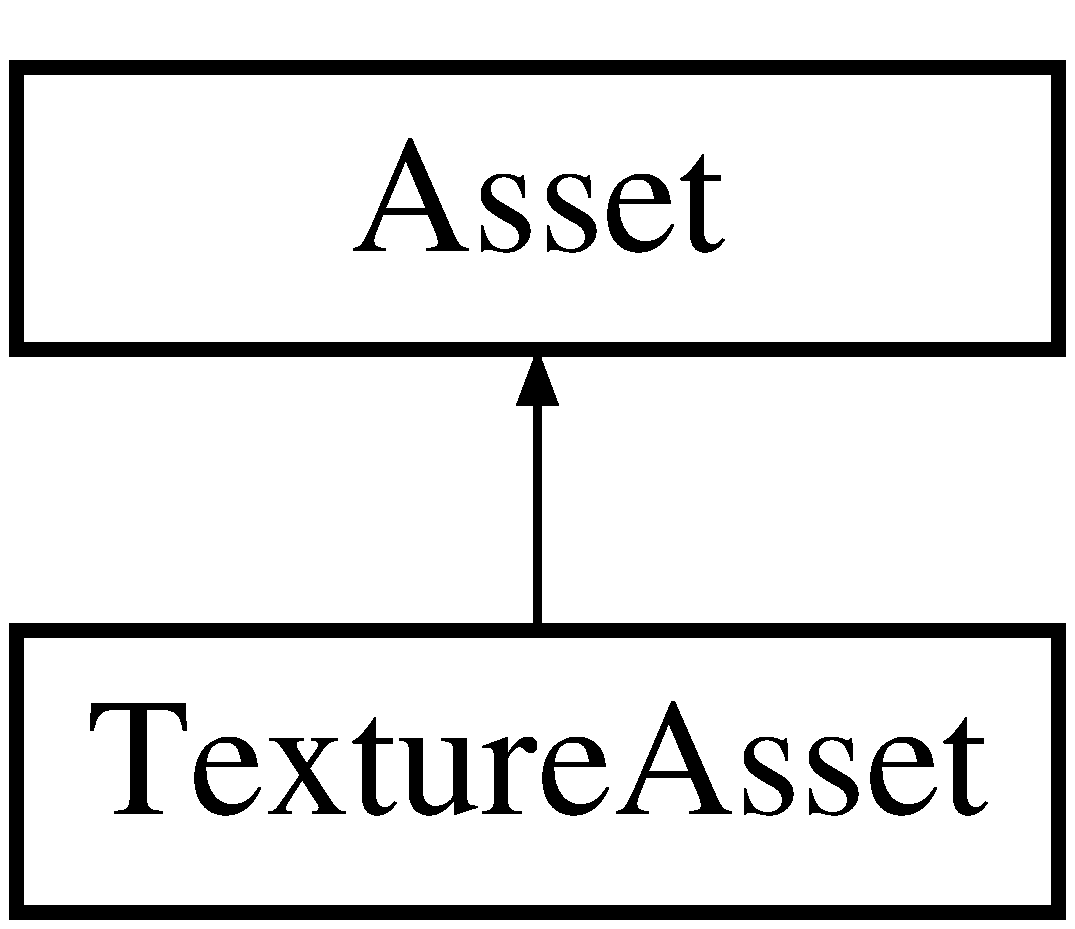
\includegraphics[height=2.000000cm]{class_texture_asset}
\end{center}
\end{figure}
\subsection*{Public Member Functions}
\begin{DoxyCompactItemize}
\item 
\mbox{\hyperlink{class_texture_asset_a09664001cf303951a8f5eb1ccc6bcd37}{Texture\+Asset}} (const std\+::string texture\+Asset\+Name)
\item 
\mbox{\hyperlink{class_texture_asset_a115d65cc1ce33a8eb9cc1762497c4537}{$\sim$\+Texture\+Asset}} ()
\item 
S\+D\+L\+\_\+\+Surface $\ast$ \mbox{\hyperlink{class_texture_asset_aef089e5da2cf3bd751e0fad708aa8d8b}{Load\+Texture\+Asset}} ()
\end{DoxyCompactItemize}
\subsection*{Additional Inherited Members}


\subsection{Detailed Description}
\mbox{\hyperlink{class_asset}{Asset}} object for loading texture assets. 

\subsection{Constructor \& Destructor Documentation}
\mbox{\Hypertarget{class_texture_asset_a09664001cf303951a8f5eb1ccc6bcd37}\label{class_texture_asset_a09664001cf303951a8f5eb1ccc6bcd37}} 
\index{Texture\+Asset@{Texture\+Asset}!Texture\+Asset@{Texture\+Asset}}
\index{Texture\+Asset@{Texture\+Asset}!Texture\+Asset@{Texture\+Asset}}
\subsubsection{\texorpdfstring{Texture\+Asset()}{TextureAsset()}}
{\footnotesize\ttfamily Texture\+Asset\+::\+Texture\+Asset (\begin{DoxyParamCaption}\item[{const std\+::string}]{texture\+Asset\+Name }\end{DoxyParamCaption})}

Constructor. \mbox{\Hypertarget{class_texture_asset_a115d65cc1ce33a8eb9cc1762497c4537}\label{class_texture_asset_a115d65cc1ce33a8eb9cc1762497c4537}} 
\index{Texture\+Asset@{Texture\+Asset}!````~Texture\+Asset@{$\sim$\+Texture\+Asset}}
\index{````~Texture\+Asset@{$\sim$\+Texture\+Asset}!Texture\+Asset@{Texture\+Asset}}
\subsubsection{\texorpdfstring{$\sim$\+Texture\+Asset()}{~TextureAsset()}}
{\footnotesize\ttfamily Texture\+Asset\+::$\sim$\+Texture\+Asset (\begin{DoxyParamCaption}{ }\end{DoxyParamCaption})}

Default destructor. 

\subsection{Member Function Documentation}
\mbox{\Hypertarget{class_texture_asset_aef089e5da2cf3bd751e0fad708aa8d8b}\label{class_texture_asset_aef089e5da2cf3bd751e0fad708aa8d8b}} 
\index{Texture\+Asset@{Texture\+Asset}!Load\+Texture\+Asset@{Load\+Texture\+Asset}}
\index{Load\+Texture\+Asset@{Load\+Texture\+Asset}!Texture\+Asset@{Texture\+Asset}}
\subsubsection{\texorpdfstring{Load\+Texture\+Asset()}{LoadTextureAsset()}}
{\footnotesize\ttfamily S\+D\+L\+\_\+\+Surface $\ast$ Texture\+Asset\+::\+Load\+Texture\+Asset (\begin{DoxyParamCaption}{ }\end{DoxyParamCaption})}

Loads a texture object. 

The documentation for this class was generated from the following files\+:\begin{DoxyCompactItemize}
\item 
Engine/\+Source/\+Runtime/\+Resource/\mbox{\hyperlink{_texture_asset_8h}{Texture\+Asset.\+h}}\item 
Engine/\+Source/\+Runtime/\+Resource/\mbox{\hyperlink{_texture_asset_8cpp}{Texture\+Asset.\+cpp}}\end{DoxyCompactItemize}

\hypertarget{struct_vec2}{}\section{Vec2 Struct Reference}
\label{struct_vec2}\index{Vec2@{Vec2}}


{\ttfamily \#include $<$Vec2.\+h$>$}

\subsection*{Public Member Functions}
\begin{DoxyCompactItemize}
\item 
\mbox{\hyperlink{struct_vec2_a76080feed7005893ecc634f903cfbae0}{Vec2}} ()
\item 
\mbox{\hyperlink{struct_vec2_a2c1181bd206d6544bf8487cf688a7096}{Vec2}} (float inX, float inY)
\item 
void \mbox{\hyperlink{struct_vec2_a0ccdf7c1f30b7e2e368860ed8530a296}{Normalize}} ()
\item 
float \mbox{\hyperlink{struct_vec2_a2d243a47e5ee4e168c71f3e013900ea8}{Size}} () const
\item 
float \mbox{\hyperlink{struct_vec2_ae3f8d3905cd5f737fa91a8dcfa250fe9}{Size\+Squared}} () const
\item 
\mbox{\hyperlink{struct_vec2}{Vec2}} \mbox{\hyperlink{struct_vec2_a65905f53c16179cea854fda5336736e2}{operator+}} (const \mbox{\hyperlink{struct_vec2}{Vec2}} \&vec)
\item 
\mbox{\hyperlink{struct_vec2}{Vec2}} \mbox{\hyperlink{struct_vec2_ab41b66fe339aae8150829626682c355e}{operator-\/}} (const \mbox{\hyperlink{struct_vec2}{Vec2}} \&vec)
\item 
\mbox{\hyperlink{struct_vec2}{Vec2}} \mbox{\hyperlink{struct_vec2_a702c5b3a06645680a94cd1929eaddca8}{operator/}} (const \mbox{\hyperlink{struct_vec2}{Vec2}} \&vec)
\item 
\mbox{\hyperlink{struct_vec2}{Vec2}} \mbox{\hyperlink{struct_vec2_a99d3335f38f28886070edacf65b45e5d}{operator$\ast$}} (const \mbox{\hyperlink{struct_vec2}{Vec2}} \&vec)
\item 
\mbox{\hyperlink{struct_vec2}{Vec2}} \mbox{\hyperlink{struct_vec2_afa88ae0d88c6bd092ca1592a06b1be04}{operator+=}} (const \mbox{\hyperlink{struct_vec2}{Vec2}} \&vec)
\item 
\mbox{\hyperlink{struct_vec2}{Vec2}} \mbox{\hyperlink{struct_vec2_a019231f7b97a2fb52c67487088fa2022}{operator-\/=}} (const \mbox{\hyperlink{struct_vec2}{Vec2}} \&vec)
\item 
\mbox{\hyperlink{struct_vec2}{Vec2}} \mbox{\hyperlink{struct_vec2_afdf4316abb4b2a286886bb1e85be783d}{operator/=}} (const \mbox{\hyperlink{struct_vec2}{Vec2}} \&vec)
\item 
\mbox{\hyperlink{struct_vec2}{Vec2}} \mbox{\hyperlink{struct_vec2_a1e277c51fc1cb0440e7b0247805c0f86}{operator$\ast$=}} (const \mbox{\hyperlink{struct_vec2}{Vec2}} \&vec)
\item 
\mbox{\hyperlink{struct_vec2}{Vec2}} \& \mbox{\hyperlink{struct_vec2_a9dfc7d928d6f12e90067538e7ac20903}{operator$\ast$}} (float scale)
\item 
\mbox{\hyperlink{struct_vec2}{Vec2}} \& \mbox{\hyperlink{struct_vec2_a4a32a53db5ca84b91028d4ee60630411}{operator$\ast$=}} (float scale)
\end{DoxyCompactItemize}
\subsection*{Public Attributes}
\begin{DoxyCompactItemize}
\item 
float \mbox{\hyperlink{struct_vec2_adf8ee322d4b4bcc04146762c018d731f}{x}}
\item 
float \mbox{\hyperlink{struct_vec2_a30543787e62f6d915543cf1dfb04c094}{y}}
\end{DoxyCompactItemize}
\subsection*{Static Public Attributes}
\begin{DoxyCompactItemize}
\item 
static const \mbox{\hyperlink{struct_vec2}{Vec2}} \mbox{\hyperlink{struct_vec2_a79378f8c63a15abc98bf639c839f345e}{zero}}
\item 
static const \mbox{\hyperlink{struct_vec2}{Vec2}} \mbox{\hyperlink{struct_vec2_a2350eb6448cb5b550f63842929423ce0}{unit}}
\end{DoxyCompactItemize}


\subsection{Constructor \& Destructor Documentation}
\mbox{\Hypertarget{struct_vec2_a76080feed7005893ecc634f903cfbae0}\label{struct_vec2_a76080feed7005893ecc634f903cfbae0}} 
\index{Vec2@{Vec2}!Vec2@{Vec2}}
\index{Vec2@{Vec2}!Vec2@{Vec2}}
\subsubsection{\texorpdfstring{Vec2()}{Vec2()}\hspace{0.1cm}{\footnotesize\ttfamily [1/2]}}
{\footnotesize\ttfamily Vec2\+::\+Vec2 (\begin{DoxyParamCaption}{ }\end{DoxyParamCaption})}

\mbox{\Hypertarget{struct_vec2_a2c1181bd206d6544bf8487cf688a7096}\label{struct_vec2_a2c1181bd206d6544bf8487cf688a7096}} 
\index{Vec2@{Vec2}!Vec2@{Vec2}}
\index{Vec2@{Vec2}!Vec2@{Vec2}}
\subsubsection{\texorpdfstring{Vec2()}{Vec2()}\hspace{0.1cm}{\footnotesize\ttfamily [2/2]}}
{\footnotesize\ttfamily Vec2\+::\+Vec2 (\begin{DoxyParamCaption}\item[{float}]{inX,  }\item[{float}]{inY }\end{DoxyParamCaption})}



\subsection{Member Function Documentation}
\mbox{\Hypertarget{struct_vec2_a0ccdf7c1f30b7e2e368860ed8530a296}\label{struct_vec2_a0ccdf7c1f30b7e2e368860ed8530a296}} 
\index{Vec2@{Vec2}!Normalize@{Normalize}}
\index{Normalize@{Normalize}!Vec2@{Vec2}}
\subsubsection{\texorpdfstring{Normalize()}{Normalize()}}
{\footnotesize\ttfamily void Vec2\+::\+Normalize (\begin{DoxyParamCaption}{ }\end{DoxyParamCaption})}

\mbox{\Hypertarget{struct_vec2_a99d3335f38f28886070edacf65b45e5d}\label{struct_vec2_a99d3335f38f28886070edacf65b45e5d}} 
\index{Vec2@{Vec2}!operator$\ast$@{operator$\ast$}}
\index{operator$\ast$@{operator$\ast$}!Vec2@{Vec2}}
\subsubsection{\texorpdfstring{operator$\ast$()}{operator*()}\hspace{0.1cm}{\footnotesize\ttfamily [1/2]}}
{\footnotesize\ttfamily \mbox{\hyperlink{struct_vec2}{Vec2}} Vec2\+::operator$\ast$ (\begin{DoxyParamCaption}\item[{const \mbox{\hyperlink{struct_vec2}{Vec2}} \&}]{vec }\end{DoxyParamCaption})}

\mbox{\Hypertarget{struct_vec2_a9dfc7d928d6f12e90067538e7ac20903}\label{struct_vec2_a9dfc7d928d6f12e90067538e7ac20903}} 
\index{Vec2@{Vec2}!operator$\ast$@{operator$\ast$}}
\index{operator$\ast$@{operator$\ast$}!Vec2@{Vec2}}
\subsubsection{\texorpdfstring{operator$\ast$()}{operator*()}\hspace{0.1cm}{\footnotesize\ttfamily [2/2]}}
{\footnotesize\ttfamily \mbox{\hyperlink{struct_vec2}{Vec2}} \& Vec2\+::operator$\ast$ (\begin{DoxyParamCaption}\item[{float}]{scale }\end{DoxyParamCaption})}

\mbox{\Hypertarget{struct_vec2_a1e277c51fc1cb0440e7b0247805c0f86}\label{struct_vec2_a1e277c51fc1cb0440e7b0247805c0f86}} 
\index{Vec2@{Vec2}!operator$\ast$=@{operator$\ast$=}}
\index{operator$\ast$=@{operator$\ast$=}!Vec2@{Vec2}}
\subsubsection{\texorpdfstring{operator$\ast$=()}{operator*=()}\hspace{0.1cm}{\footnotesize\ttfamily [1/2]}}
{\footnotesize\ttfamily \mbox{\hyperlink{struct_vec2}{Vec2}} Vec2\+::operator$\ast$= (\begin{DoxyParamCaption}\item[{const \mbox{\hyperlink{struct_vec2}{Vec2}} \&}]{vec }\end{DoxyParamCaption})}

\mbox{\Hypertarget{struct_vec2_a4a32a53db5ca84b91028d4ee60630411}\label{struct_vec2_a4a32a53db5ca84b91028d4ee60630411}} 
\index{Vec2@{Vec2}!operator$\ast$=@{operator$\ast$=}}
\index{operator$\ast$=@{operator$\ast$=}!Vec2@{Vec2}}
\subsubsection{\texorpdfstring{operator$\ast$=()}{operator*=()}\hspace{0.1cm}{\footnotesize\ttfamily [2/2]}}
{\footnotesize\ttfamily \mbox{\hyperlink{struct_vec2}{Vec2}} \& Vec2\+::operator$\ast$= (\begin{DoxyParamCaption}\item[{float}]{scale }\end{DoxyParamCaption})}

\mbox{\Hypertarget{struct_vec2_a65905f53c16179cea854fda5336736e2}\label{struct_vec2_a65905f53c16179cea854fda5336736e2}} 
\index{Vec2@{Vec2}!operator+@{operator+}}
\index{operator+@{operator+}!Vec2@{Vec2}}
\subsubsection{\texorpdfstring{operator+()}{operator+()}}
{\footnotesize\ttfamily \mbox{\hyperlink{struct_vec2}{Vec2}} Vec2\+::operator+ (\begin{DoxyParamCaption}\item[{const \mbox{\hyperlink{struct_vec2}{Vec2}} \&}]{vec }\end{DoxyParamCaption})}

\mbox{\Hypertarget{struct_vec2_afa88ae0d88c6bd092ca1592a06b1be04}\label{struct_vec2_afa88ae0d88c6bd092ca1592a06b1be04}} 
\index{Vec2@{Vec2}!operator+=@{operator+=}}
\index{operator+=@{operator+=}!Vec2@{Vec2}}
\subsubsection{\texorpdfstring{operator+=()}{operator+=()}}
{\footnotesize\ttfamily \mbox{\hyperlink{struct_vec2}{Vec2}} Vec2\+::operator+= (\begin{DoxyParamCaption}\item[{const \mbox{\hyperlink{struct_vec2}{Vec2}} \&}]{vec }\end{DoxyParamCaption})}

\mbox{\Hypertarget{struct_vec2_ab41b66fe339aae8150829626682c355e}\label{struct_vec2_ab41b66fe339aae8150829626682c355e}} 
\index{Vec2@{Vec2}!operator-\/@{operator-\/}}
\index{operator-\/@{operator-\/}!Vec2@{Vec2}}
\subsubsection{\texorpdfstring{operator-\/()}{operator-()}}
{\footnotesize\ttfamily \mbox{\hyperlink{struct_vec2}{Vec2}} Vec2\+::operator-\/ (\begin{DoxyParamCaption}\item[{const \mbox{\hyperlink{struct_vec2}{Vec2}} \&}]{vec }\end{DoxyParamCaption})}

\mbox{\Hypertarget{struct_vec2_a019231f7b97a2fb52c67487088fa2022}\label{struct_vec2_a019231f7b97a2fb52c67487088fa2022}} 
\index{Vec2@{Vec2}!operator-\/=@{operator-\/=}}
\index{operator-\/=@{operator-\/=}!Vec2@{Vec2}}
\subsubsection{\texorpdfstring{operator-\/=()}{operator-=()}}
{\footnotesize\ttfamily \mbox{\hyperlink{struct_vec2}{Vec2}} Vec2\+::operator-\/= (\begin{DoxyParamCaption}\item[{const \mbox{\hyperlink{struct_vec2}{Vec2}} \&}]{vec }\end{DoxyParamCaption})}

\mbox{\Hypertarget{struct_vec2_a702c5b3a06645680a94cd1929eaddca8}\label{struct_vec2_a702c5b3a06645680a94cd1929eaddca8}} 
\index{Vec2@{Vec2}!operator/@{operator/}}
\index{operator/@{operator/}!Vec2@{Vec2}}
\subsubsection{\texorpdfstring{operator/()}{operator/()}}
{\footnotesize\ttfamily \mbox{\hyperlink{struct_vec2}{Vec2}} Vec2\+::operator/ (\begin{DoxyParamCaption}\item[{const \mbox{\hyperlink{struct_vec2}{Vec2}} \&}]{vec }\end{DoxyParamCaption})}

\mbox{\Hypertarget{struct_vec2_afdf4316abb4b2a286886bb1e85be783d}\label{struct_vec2_afdf4316abb4b2a286886bb1e85be783d}} 
\index{Vec2@{Vec2}!operator/=@{operator/=}}
\index{operator/=@{operator/=}!Vec2@{Vec2}}
\subsubsection{\texorpdfstring{operator/=()}{operator/=()}}
{\footnotesize\ttfamily \mbox{\hyperlink{struct_vec2}{Vec2}} Vec2\+::operator/= (\begin{DoxyParamCaption}\item[{const \mbox{\hyperlink{struct_vec2}{Vec2}} \&}]{vec }\end{DoxyParamCaption})}

\mbox{\Hypertarget{struct_vec2_a2d243a47e5ee4e168c71f3e013900ea8}\label{struct_vec2_a2d243a47e5ee4e168c71f3e013900ea8}} 
\index{Vec2@{Vec2}!Size@{Size}}
\index{Size@{Size}!Vec2@{Vec2}}
\subsubsection{\texorpdfstring{Size()}{Size()}}
{\footnotesize\ttfamily float Vec2\+::\+Size (\begin{DoxyParamCaption}{ }\end{DoxyParamCaption}) const}

\mbox{\Hypertarget{struct_vec2_ae3f8d3905cd5f737fa91a8dcfa250fe9}\label{struct_vec2_ae3f8d3905cd5f737fa91a8dcfa250fe9}} 
\index{Vec2@{Vec2}!Size\+Squared@{Size\+Squared}}
\index{Size\+Squared@{Size\+Squared}!Vec2@{Vec2}}
\subsubsection{\texorpdfstring{Size\+Squared()}{SizeSquared()}}
{\footnotesize\ttfamily float Vec2\+::\+Size\+Squared (\begin{DoxyParamCaption}{ }\end{DoxyParamCaption}) const}



\subsection{Member Data Documentation}
\mbox{\Hypertarget{struct_vec2_a2350eb6448cb5b550f63842929423ce0}\label{struct_vec2_a2350eb6448cb5b550f63842929423ce0}} 
\index{Vec2@{Vec2}!unit@{unit}}
\index{unit@{unit}!Vec2@{Vec2}}
\subsubsection{\texorpdfstring{unit}{unit}}
{\footnotesize\ttfamily const \mbox{\hyperlink{struct_vec2}{Vec2}} Vec2\+::unit\hspace{0.3cm}{\ttfamily [static]}}

\mbox{\Hypertarget{struct_vec2_adf8ee322d4b4bcc04146762c018d731f}\label{struct_vec2_adf8ee322d4b4bcc04146762c018d731f}} 
\index{Vec2@{Vec2}!x@{x}}
\index{x@{x}!Vec2@{Vec2}}
\subsubsection{\texorpdfstring{x}{x}}
{\footnotesize\ttfamily float Vec2\+::x}

\mbox{\Hypertarget{struct_vec2_a30543787e62f6d915543cf1dfb04c094}\label{struct_vec2_a30543787e62f6d915543cf1dfb04c094}} 
\index{Vec2@{Vec2}!y@{y}}
\index{y@{y}!Vec2@{Vec2}}
\subsubsection{\texorpdfstring{y}{y}}
{\footnotesize\ttfamily float Vec2\+::y}

\mbox{\Hypertarget{struct_vec2_a79378f8c63a15abc98bf639c839f345e}\label{struct_vec2_a79378f8c63a15abc98bf639c839f345e}} 
\index{Vec2@{Vec2}!zero@{zero}}
\index{zero@{zero}!Vec2@{Vec2}}
\subsubsection{\texorpdfstring{zero}{zero}}
{\footnotesize\ttfamily const \mbox{\hyperlink{struct_vec2}{Vec2}} Vec2\+::zero\hspace{0.3cm}{\ttfamily [static]}}



The documentation for this struct was generated from the following files\+:\begin{DoxyCompactItemize}
\item 
Engine/\+Source/\+Runtime/\+Math/\mbox{\hyperlink{_vec2_8h}{Vec2.\+h}}\item 
Engine/\+Source/\+Runtime/\+Math/\mbox{\hyperlink{_vec2_8cpp}{Vec2.\+cpp}}\end{DoxyCompactItemize}

\hypertarget{class_world}{}\section{World Class Reference}
\label{class_world}\index{World@{World}}


{\ttfamily \#include $<$World.\+h$>$}

\subsection*{Public Member Functions}
\begin{DoxyCompactItemize}
\item 
\mbox{\hyperlink{class_world_afa39d4e6f714a7a3691ac0c656f5e8a8}{World}} ()
\item 
\mbox{\hyperlink{class_world_a8c73fba541a5817fff65147ba47cd827}{$\sim$\+World}} ()
\item 
void \mbox{\hyperlink{class_world_a72d413fcf9f301d1e2613844fd60f058}{Initialize}} (S\+D\+L\+\_\+\+Renderer $\ast$renderer)
\item 
void \mbox{\hyperlink{class_world_afdb5329b573ec0d74ba38e4641977705}{Update}} (float delta\+Time)
\item 
void \mbox{\hyperlink{class_world_ac42466df32c2d68dc36c41b3e1e9cdad}{Draw}} (S\+D\+L\+\_\+\+Renderer $\ast$renderer)
\end{DoxyCompactItemize}


\subsection{Detailed Description}
A world is a high level game object that represents a game level. 

\subsection{Constructor \& Destructor Documentation}
\mbox{\Hypertarget{class_world_afa39d4e6f714a7a3691ac0c656f5e8a8}\label{class_world_afa39d4e6f714a7a3691ac0c656f5e8a8}} 
\index{World@{World}!World@{World}}
\index{World@{World}!World@{World}}
\subsubsection{\texorpdfstring{World()}{World()}}
{\footnotesize\ttfamily World\+::\+World (\begin{DoxyParamCaption}{ }\end{DoxyParamCaption})}

Default constructor. \mbox{\Hypertarget{class_world_a8c73fba541a5817fff65147ba47cd827}\label{class_world_a8c73fba541a5817fff65147ba47cd827}} 
\index{World@{World}!````~World@{$\sim$\+World}}
\index{````~World@{$\sim$\+World}!World@{World}}
\subsubsection{\texorpdfstring{$\sim$\+World()}{~World()}}
{\footnotesize\ttfamily World\+::$\sim$\+World (\begin{DoxyParamCaption}{ }\end{DoxyParamCaption})}

Default destructor. 

\subsection{Member Function Documentation}
\mbox{\Hypertarget{class_world_ac42466df32c2d68dc36c41b3e1e9cdad}\label{class_world_ac42466df32c2d68dc36c41b3e1e9cdad}} 
\index{World@{World}!Draw@{Draw}}
\index{Draw@{Draw}!World@{World}}
\subsubsection{\texorpdfstring{Draw()}{Draw()}}
{\footnotesize\ttfamily void World\+::\+Draw (\begin{DoxyParamCaption}\item[{S\+D\+L\+\_\+\+Renderer $\ast$}]{renderer }\end{DoxyParamCaption})}

Draw all game objects in the game world. \mbox{\Hypertarget{class_world_a72d413fcf9f301d1e2613844fd60f058}\label{class_world_a72d413fcf9f301d1e2613844fd60f058}} 
\index{World@{World}!Initialize@{Initialize}}
\index{Initialize@{Initialize}!World@{World}}
\subsubsection{\texorpdfstring{Initialize()}{Initialize()}}
{\footnotesize\ttfamily void World\+::\+Initialize (\begin{DoxyParamCaption}\item[{S\+D\+L\+\_\+\+Renderer $\ast$}]{renderer }\end{DoxyParamCaption})}

Initialize the game world object. \mbox{\Hypertarget{class_world_afdb5329b573ec0d74ba38e4641977705}\label{class_world_afdb5329b573ec0d74ba38e4641977705}} 
\index{World@{World}!Update@{Update}}
\index{Update@{Update}!World@{World}}
\subsubsection{\texorpdfstring{Update()}{Update()}}
{\footnotesize\ttfamily void World\+::\+Update (\begin{DoxyParamCaption}\item[{float}]{delta\+Time }\end{DoxyParamCaption})}

Update all game objects in the game world, called once per frame. 

The documentation for this class was generated from the following files\+:\begin{DoxyCompactItemize}
\item 
Engine/\+Source/\+Runtime/\+Game\+Object/\mbox{\hyperlink{_world_8h}{World.\+h}}\item 
Engine/\+Source/\+Runtime/\+Game\+Object/\mbox{\hyperlink{_world_8cpp}{World.\+cpp}}\end{DoxyCompactItemize}

\hypertarget{class_world_loader}{}\section{World\+Loader Class Reference}
\label{class_world_loader}\index{World\+Loader@{World\+Loader}}


{\ttfamily \#include $<$World\+Loader.\+h$>$}

\subsection*{Static Public Member Functions}
\begin{DoxyCompactItemize}
\item 
static bool \mbox{\hyperlink{class_world_loader_a1e5dea70d3a7d5d75d352a5041c3f86a}{Load\+World}} (const std\+::string \&filename)
\end{DoxyCompactItemize}


\subsection{Member Function Documentation}
\mbox{\Hypertarget{class_world_loader_a1e5dea70d3a7d5d75d352a5041c3f86a}\label{class_world_loader_a1e5dea70d3a7d5d75d352a5041c3f86a}} 
\index{World\+Loader@{World\+Loader}!Load\+World@{Load\+World}}
\index{Load\+World@{Load\+World}!World\+Loader@{World\+Loader}}
\subsubsection{\texorpdfstring{Load\+World()}{LoadWorld()}}
{\footnotesize\ttfamily bool World\+Loader\+::\+Load\+World (\begin{DoxyParamCaption}\item[{const std\+::string \&}]{filename }\end{DoxyParamCaption})\hspace{0.3cm}{\ttfamily [static]}}

Loads a world object from a J\+S\+ON file object. 

The documentation for this class was generated from the following files\+:\begin{DoxyCompactItemize}
\item 
Engine/\+Source/\+Runtime/\+Game\+Object/\mbox{\hyperlink{_world_loader_8h}{World\+Loader.\+h}}\item 
Engine/\+Source/\+Runtime/\+Game\+Object/\mbox{\hyperlink{_world_loader_8cpp}{World\+Loader.\+cpp}}\end{DoxyCompactItemize}

\chapter{File Documentation}
\hypertarget{_a_i_behavior_8cpp}{}\section{Engine/\+Source/\+Runtime/\+A\+I/\+A\+I\+Behavior.cpp File Reference}
\label{_a_i_behavior_8cpp}\index{Engine/\+Source/\+Runtime/\+A\+I/\+A\+I\+Behavior.\+cpp@{Engine/\+Source/\+Runtime/\+A\+I/\+A\+I\+Behavior.\+cpp}}
{\ttfamily \#include \char`\"{}stdafx.\+h\char`\"{}}\newline
{\ttfamily \#include \char`\"{}A\+I\+Behavior.\+h\char`\"{}}\newline
{\ttfamily \#include \char`\"{}Game\+Object/\+Entity.\+h\char`\"{}}\newline

\hypertarget{_a_i_behavior_8h}{}\section{Engine/\+Source/\+Runtime/\+A\+I/\+A\+I\+Behavior.h File Reference}
\label{_a_i_behavior_8h}\index{Engine/\+Source/\+Runtime/\+A\+I/\+A\+I\+Behavior.\+h@{Engine/\+Source/\+Runtime/\+A\+I/\+A\+I\+Behavior.\+h}}
{\ttfamily \#include \char`\"{}Math/\+Vec2.\+h\char`\"{}}\newline
\subsection*{Classes}
\begin{DoxyCompactItemize}
\item 
class \mbox{\hyperlink{class_a_i_behavior}{A\+I\+Behavior}}
\end{DoxyCompactItemize}

\hypertarget{_a_i_component_8cpp}{}\section{Engine/\+Source/\+Runtime/\+A\+I/\+A\+I\+Component.cpp File Reference}
\label{_a_i_component_8cpp}\index{Engine/\+Source/\+Runtime/\+A\+I/\+A\+I\+Component.\+cpp@{Engine/\+Source/\+Runtime/\+A\+I/\+A\+I\+Component.\+cpp}}
{\ttfamily \#include \char`\"{}stdafx.\+h\char`\"{}}\newline
{\ttfamily \#include \char`\"{}A\+I\+Component.\+h\char`\"{}}\newline
{\ttfamily \#include \char`\"{}A\+I\+Behavior.\+h\char`\"{}}\newline

\hypertarget{_a_i_component_8h}{}\section{Engine/\+Source/\+Runtime/\+A\+I/\+A\+I\+Component.h File Reference}
\label{_a_i_component_8h}\index{Engine/\+Source/\+Runtime/\+A\+I/\+A\+I\+Component.\+h@{Engine/\+Source/\+Runtime/\+A\+I/\+A\+I\+Component.\+h}}
{\ttfamily \#include \char`\"{}Game\+Object/\+Component.\+h\char`\"{}}\newline
\subsection*{Classes}
\begin{DoxyCompactItemize}
\item 
class \mbox{\hyperlink{class_a_i_component}{A\+I\+Component}}
\end{DoxyCompactItemize}

\hypertarget{_audio_cue_8cpp}{}\section{Engine/\+Source/\+Runtime/\+Audio/\+Audio\+Cue.cpp File Reference}
\label{_audio_cue_8cpp}\index{Engine/\+Source/\+Runtime/\+Audio/\+Audio\+Cue.\+cpp@{Engine/\+Source/\+Runtime/\+Audio/\+Audio\+Cue.\+cpp}}
{\ttfamily \#include \char`\"{}stdafx.\+h\char`\"{}}\newline
{\ttfamily \#include \char`\"{}Audio\+Cue.\+h\char`\"{}}\newline

\hypertarget{_audio_cue_8h}{}\section{Engine/\+Source/\+Runtime/\+Audio/\+Audio\+Cue.h File Reference}
\label{_audio_cue_8h}\index{Engine/\+Source/\+Runtime/\+Audio/\+Audio\+Cue.\+h@{Engine/\+Source/\+Runtime/\+Audio/\+Audio\+Cue.\+h}}
\subsection*{Classes}
\begin{DoxyCompactItemize}
\item 
class \mbox{\hyperlink{class_audio_cue}{Audio\+Cue}}
\end{DoxyCompactItemize}

\hypertarget{_audio_manager_8cpp}{}\section{Engine/\+Source/\+Runtime/\+Audio/\+Audio\+Manager.cpp File Reference}
\label{_audio_manager_8cpp}\index{Engine/\+Source/\+Runtime/\+Audio/\+Audio\+Manager.\+cpp@{Engine/\+Source/\+Runtime/\+Audio/\+Audio\+Manager.\+cpp}}
{\ttfamily \#include \char`\"{}stdafx.\+h\char`\"{}}\newline
{\ttfamily \#include \char`\"{}Audio\+Manager.\+h\char`\"{}}\newline

\hypertarget{_audio_manager_8h}{}\section{Engine/\+Source/\+Runtime/\+Audio/\+Audio\+Manager.h File Reference}
\label{_audio_manager_8h}\index{Engine/\+Source/\+Runtime/\+Audio/\+Audio\+Manager.\+h@{Engine/\+Source/\+Runtime/\+Audio/\+Audio\+Manager.\+h}}
\subsection*{Classes}
\begin{DoxyCompactItemize}
\item 
class \mbox{\hyperlink{class_audio_manager}{Audio\+Manager}}
\end{DoxyCompactItemize}

\hypertarget{_config_8h}{}\section{Engine/\+Source/\+Runtime/\+Core/\+Config.h File Reference}
\label{_config_8h}\index{Engine/\+Source/\+Runtime/\+Core/\+Config.\+h@{Engine/\+Source/\+Runtime/\+Core/\+Config.\+h}}

\hypertarget{_game_app_8cpp}{}\section{Engine/\+Source/\+Runtime/\+Core/\+Game\+App.cpp File Reference}
\label{_game_app_8cpp}\index{Engine/\+Source/\+Runtime/\+Core/\+Game\+App.\+cpp@{Engine/\+Source/\+Runtime/\+Core/\+Game\+App.\+cpp}}
{\ttfamily \#include \char`\"{}stdafx.\+h\char`\"{}}\newline
{\ttfamily \#include \char`\"{}Game\+App.\+h\char`\"{}}\newline
{\ttfamily \#include \char`\"{}Renderer.\+h\char`\"{}}\newline
{\ttfamily \#include \char`\"{}Game\+Object/\+World.\+h\char`\"{}}\newline
{\ttfamily \#include \char`\"{}Resource/\+Asset\+Manager.\+h\char`\"{}}\newline
{\ttfamily \#include \char`\"{}Resource/\+Texture\+Asset.\+h\char`\"{}}\newline
{\ttfamily \#include \char`\"{}Config.\+h\char`\"{}}\newline

\hypertarget{_game_app_8h}{}\section{Engine/\+Source/\+Runtime/\+Core/\+Game\+App.h File Reference}
\label{_game_app_8h}\index{Engine/\+Source/\+Runtime/\+Core/\+Game\+App.\+h@{Engine/\+Source/\+Runtime/\+Core/\+Game\+App.\+h}}
\subsection*{Classes}
\begin{DoxyCompactItemize}
\item 
class \mbox{\hyperlink{class_asset_manager}{Asset\+Manager$<$ T $>$}}
\item 
class \mbox{\hyperlink{class_game_app}{Game\+App}}
\end{DoxyCompactItemize}
\subsection*{Enumerations}
\begin{DoxyCompactItemize}
\item 
enum \mbox{\hyperlink{_game_app_8h_a58dc439d7f01a8000901a1d441cb3521}{E\+Window\+Mode}} \{ \mbox{\hyperlink{_game_app_8h_a58dc439d7f01a8000901a1d441cb3521a5a9d2e2d78c543644a09237425f01b1b}{E\+Fullscreen}}, 
\mbox{\hyperlink{_game_app_8h_a58dc439d7f01a8000901a1d441cb3521a91e8d2aca9a3d6b244ae31a4c5fb1adb}{E\+Windowed}}
 \}
\end{DoxyCompactItemize}


\subsection{Enumeration Type Documentation}
\mbox{\Hypertarget{_game_app_8h_a58dc439d7f01a8000901a1d441cb3521}\label{_game_app_8h_a58dc439d7f01a8000901a1d441cb3521}} 
\index{Game\+App.\+h@{Game\+App.\+h}!E\+Window\+Mode@{E\+Window\+Mode}}
\index{E\+Window\+Mode@{E\+Window\+Mode}!Game\+App.\+h@{Game\+App.\+h}}
\subsubsection{\texorpdfstring{E\+Window\+Mode}{EWindowMode}}
{\footnotesize\ttfamily enum \mbox{\hyperlink{_game_app_8h_a58dc439d7f01a8000901a1d441cb3521}{E\+Window\+Mode}}}

Mode the window is currently in \begin{DoxyEnumFields}{Enumerator}
\raisebox{\heightof{T}}[0pt][0pt]{\index{E\+Fullscreen@{E\+Fullscreen}!Game\+App.\+h@{Game\+App.\+h}}\index{Game\+App.\+h@{Game\+App.\+h}!E\+Fullscreen@{E\+Fullscreen}}}\mbox{\Hypertarget{_game_app_8h_a58dc439d7f01a8000901a1d441cb3521a5a9d2e2d78c543644a09237425f01b1b}\label{_game_app_8h_a58dc439d7f01a8000901a1d441cb3521a5a9d2e2d78c543644a09237425f01b1b}} 
E\+Fullscreen&\\
\hline

\raisebox{\heightof{T}}[0pt][0pt]{\index{E\+Windowed@{E\+Windowed}!Game\+App.\+h@{Game\+App.\+h}}\index{Game\+App.\+h@{Game\+App.\+h}!E\+Windowed@{E\+Windowed}}}\mbox{\Hypertarget{_game_app_8h_a58dc439d7f01a8000901a1d441cb3521a91e8d2aca9a3d6b244ae31a4c5fb1adb}\label{_game_app_8h_a58dc439d7f01a8000901a1d441cb3521a91e8d2aca9a3d6b244ae31a4c5fb1adb}} 
E\+Windowed&\\
\hline

\end{DoxyEnumFields}

\hypertarget{_renderer_8cpp}{}\section{Engine/\+Source/\+Runtime/\+Core/\+Renderer.cpp File Reference}
\label{_renderer_8cpp}\index{Engine/\+Source/\+Runtime/\+Core/\+Renderer.\+cpp@{Engine/\+Source/\+Runtime/\+Core/\+Renderer.\+cpp}}
{\ttfamily \#include \char`\"{}stdafx.\+h\char`\"{}}\newline
{\ttfamily \#include \char`\"{}Renderer.\+h\char`\"{}}\newline

\hypertarget{_renderer_8h}{}\section{Engine/\+Source/\+Runtime/\+Core/\+Renderer.h File Reference}
\label{_renderer_8h}\index{Engine/\+Source/\+Runtime/\+Core/\+Renderer.\+h@{Engine/\+Source/\+Runtime/\+Core/\+Renderer.\+h}}
\subsection*{Classes}
\begin{DoxyCompactItemize}
\item 
class \mbox{\hyperlink{class_renderer}{Renderer}}
\end{DoxyCompactItemize}

\hypertarget{_event_8cpp}{}\section{Engine/\+Source/\+Runtime/\+Event\+System/\+Event.cpp File Reference}
\label{_event_8cpp}\index{Engine/\+Source/\+Runtime/\+Event\+System/\+Event.\+cpp@{Engine/\+Source/\+Runtime/\+Event\+System/\+Event.\+cpp}}
{\ttfamily \#include \char`\"{}stdafx.\+h\char`\"{}}\newline
{\ttfamily \#include \char`\"{}Event.\+h\char`\"{}}\newline

\hypertarget{_event_8h}{}\section{Engine/\+Source/\+Runtime/\+Event\+System/\+Event.h File Reference}
\label{_event_8h}\index{Engine/\+Source/\+Runtime/\+Event\+System/\+Event.\+h@{Engine/\+Source/\+Runtime/\+Event\+System/\+Event.\+h}}
\subsection*{Classes}
\begin{DoxyCompactItemize}
\item 
class \mbox{\hyperlink{class_event}{Event}}
\end{DoxyCompactItemize}

\hypertarget{_event_dispatcher_8h}{}\section{Engine/\+Source/\+Runtime/\+Event\+System/\+Event\+Dispatcher.h File Reference}
\label{_event_dispatcher_8h}\index{Engine/\+Source/\+Runtime/\+Event\+System/\+Event\+Dispatcher.\+h@{Engine/\+Source/\+Runtime/\+Event\+System/\+Event\+Dispatcher.\+h}}
\subsection*{Classes}
\begin{DoxyCompactItemize}
\item 
class \mbox{\hyperlink{class_event_dispatcher}{Event\+Dispatcher}}
\end{DoxyCompactItemize}

\hypertarget{_event_listener_8h}{}\section{Engine/\+Source/\+Runtime/\+Event\+System/\+Event\+Listener.h File Reference}
\label{_event_listener_8h}\index{Engine/\+Source/\+Runtime/\+Event\+System/\+Event\+Listener.\+h@{Engine/\+Source/\+Runtime/\+Event\+System/\+Event\+Listener.\+h}}
\subsection*{Classes}
\begin{DoxyCompactItemize}
\item 
class \mbox{\hyperlink{class_i_event_listener}{I\+Event\+Listener}}
\end{DoxyCompactItemize}

\hypertarget{_component_8cpp}{}\section{Engine/\+Source/\+Runtime/\+Game\+Object/\+Component.cpp File Reference}
\label{_component_8cpp}\index{Engine/\+Source/\+Runtime/\+Game\+Object/\+Component.\+cpp@{Engine/\+Source/\+Runtime/\+Game\+Object/\+Component.\+cpp}}
{\ttfamily \#include \char`\"{}stdafx.\+h\char`\"{}}\newline
{\ttfamily \#include \char`\"{}Component.\+h\char`\"{}}\newline

\hypertarget{_component_8h}{}\section{Engine/\+Source/\+Runtime/\+Game\+Object/\+Component.h File Reference}
\label{_component_8h}\index{Engine/\+Source/\+Runtime/\+Game\+Object/\+Component.\+h@{Engine/\+Source/\+Runtime/\+Game\+Object/\+Component.\+h}}
\subsection*{Classes}
\begin{DoxyCompactItemize}
\item 
class \mbox{\hyperlink{class_component}{Component}}
\end{DoxyCompactItemize}

\hypertarget{_component_manager_8cpp}{}\section{Engine/\+Source/\+Runtime/\+Game\+Object/\+Component\+Manager.cpp File Reference}
\label{_component_manager_8cpp}\index{Engine/\+Source/\+Runtime/\+Game\+Object/\+Component\+Manager.\+cpp@{Engine/\+Source/\+Runtime/\+Game\+Object/\+Component\+Manager.\+cpp}}
{\ttfamily \#include \char`\"{}stdafx.\+h\char`\"{}}\newline
{\ttfamily \#include \char`\"{}Component\+Manager.\+h\char`\"{}}\newline

\hypertarget{_component_manager_8h}{}\section{Engine/\+Source/\+Runtime/\+Game\+Object/\+Component\+Manager.h File Reference}
\label{_component_manager_8h}\index{Engine/\+Source/\+Runtime/\+Game\+Object/\+Component\+Manager.\+h@{Engine/\+Source/\+Runtime/\+Game\+Object/\+Component\+Manager.\+h}}
\subsection*{Classes}
\begin{DoxyCompactItemize}
\item 
class \mbox{\hyperlink{class_component_manager}{Component\+Manager}}
\end{DoxyCompactItemize}

\hypertarget{_collision_component_8cpp}{}\section{Engine/\+Source/\+Runtime/\+Game\+Object/\+Components/\+Collision\+Component.cpp File Reference}
\label{_collision_component_8cpp}\index{Engine/\+Source/\+Runtime/\+Game\+Object/\+Components/\+Collision\+Component.\+cpp@{Engine/\+Source/\+Runtime/\+Game\+Object/\+Components/\+Collision\+Component.\+cpp}}
{\ttfamily \#include \char`\"{}stdafx.\+h\char`\"{}}\newline
{\ttfamily \#include \char`\"{}Collision\+Component.\+h\char`\"{}}\newline

\hypertarget{_collision_component_8h}{}\section{Engine/\+Source/\+Runtime/\+Game\+Object/\+Components/\+Collision\+Component.h File Reference}
\label{_collision_component_8h}\index{Engine/\+Source/\+Runtime/\+Game\+Object/\+Components/\+Collision\+Component.\+h@{Engine/\+Source/\+Runtime/\+Game\+Object/\+Components/\+Collision\+Component.\+h}}
{\ttfamily \#include \char`\"{}Game\+Object/\+Component.\+h\char`\"{}}\newline
\subsection*{Classes}
\begin{DoxyCompactItemize}
\item 
class \mbox{\hyperlink{class_collision_component}{Collision\+Component}}
\end{DoxyCompactItemize}

\hypertarget{_input_component_8cpp}{}\section{Engine/\+Source/\+Runtime/\+Game\+Object/\+Components/\+Input\+Component.cpp File Reference}
\label{_input_component_8cpp}\index{Engine/\+Source/\+Runtime/\+Game\+Object/\+Components/\+Input\+Component.\+cpp@{Engine/\+Source/\+Runtime/\+Game\+Object/\+Components/\+Input\+Component.\+cpp}}
{\ttfamily \#include \char`\"{}stdafx.\+h\char`\"{}}\newline
{\ttfamily \#include \char`\"{}Input\+Component.\+h\char`\"{}}\newline
{\ttfamily \#include \char`\"{}Input/\+Gamepad.\+h\char`\"{}}\newline

\hypertarget{_input_component_8h}{}\section{Engine/\+Source/\+Runtime/\+Game\+Object/\+Components/\+Input\+Component.h File Reference}
\label{_input_component_8h}\index{Engine/\+Source/\+Runtime/\+Game\+Object/\+Components/\+Input\+Component.\+h@{Engine/\+Source/\+Runtime/\+Game\+Object/\+Components/\+Input\+Component.\+h}}
{\ttfamily \#include \char`\"{}Game\+Object/\+Component.\+h\char`\"{}}\newline
\subsection*{Classes}
\begin{DoxyCompactItemize}
\item 
class \mbox{\hyperlink{class_input_component}{Input\+Component}}
\end{DoxyCompactItemize}

\hypertarget{_sprite_component_8cpp}{}\section{Engine/\+Source/\+Runtime/\+Game\+Object/\+Components/\+Sprite\+Component.cpp File Reference}
\label{_sprite_component_8cpp}\index{Engine/\+Source/\+Runtime/\+Game\+Object/\+Components/\+Sprite\+Component.\+cpp@{Engine/\+Source/\+Runtime/\+Game\+Object/\+Components/\+Sprite\+Component.\+cpp}}
{\ttfamily \#include \char`\"{}stdafx.\+h\char`\"{}}\newline
{\ttfamily \#include \char`\"{}Sprite\+Component.\+h\char`\"{}}\newline
{\ttfamily \#include \char`\"{}Core/\+Renderer.\+h\char`\"{}}\newline
{\ttfamily \#include \char`\"{}Resource/\+Asset\+Manager.\+h\char`\"{}}\newline
{\ttfamily \#include \char`\"{}Resource/\+Texture\+Asset.\+h\char`\"{}}\newline
{\ttfamily \#include \char`\"{}Game\+Object/\+Entity.\+h\char`\"{}}\newline

\hypertarget{_sprite_component_8h}{}\section{Engine/\+Source/\+Runtime/\+Game\+Object/\+Components/\+Sprite\+Component.h File Reference}
\label{_sprite_component_8h}\index{Engine/\+Source/\+Runtime/\+Game\+Object/\+Components/\+Sprite\+Component.\+h@{Engine/\+Source/\+Runtime/\+Game\+Object/\+Components/\+Sprite\+Component.\+h}}
{\ttfamily \#include \char`\"{}Game\+Object/\+Component.\+h\char`\"{}}\newline
\subsection*{Classes}
\begin{DoxyCompactItemize}
\item 
class \mbox{\hyperlink{class_sprite_component}{Sprite\+Component}}
\end{DoxyCompactItemize}

\hypertarget{_entity_8cpp}{}\section{Engine/\+Source/\+Runtime/\+Game\+Object/\+Entity.cpp File Reference}
\label{_entity_8cpp}\index{Engine/\+Source/\+Runtime/\+Game\+Object/\+Entity.\+cpp@{Engine/\+Source/\+Runtime/\+Game\+Object/\+Entity.\+cpp}}
{\ttfamily \#include \char`\"{}stdafx.\+h\char`\"{}}\newline
{\ttfamily \#include \char`\"{}Entity.\+h\char`\"{}}\newline

\hypertarget{_entity_8h}{}\section{Engine/\+Source/\+Runtime/\+Game\+Object/\+Entity.h File Reference}
\label{_entity_8h}\index{Engine/\+Source/\+Runtime/\+Game\+Object/\+Entity.\+h@{Engine/\+Source/\+Runtime/\+Game\+Object/\+Entity.\+h}}
{\ttfamily \#include \char`\"{}Math/\+Vec2.\+h\char`\"{}}\newline
\subsection*{Classes}
\begin{DoxyCompactItemize}
\item 
class \mbox{\hyperlink{class_entity}{Entity}}
\end{DoxyCompactItemize}

\hypertarget{_entity_manager_8cpp}{}\section{Engine/\+Source/\+Runtime/\+Game\+Object/\+Entity\+Manager.cpp File Reference}
\label{_entity_manager_8cpp}\index{Engine/\+Source/\+Runtime/\+Game\+Object/\+Entity\+Manager.\+cpp@{Engine/\+Source/\+Runtime/\+Game\+Object/\+Entity\+Manager.\+cpp}}
{\ttfamily \#include \char`\"{}stdafx.\+h\char`\"{}}\newline
{\ttfamily \#include \char`\"{}Entity\+Manager.\+h\char`\"{}}\newline
{\ttfamily \#include \char`\"{}Entity.\+h\char`\"{}}\newline

\hypertarget{_entity_manager_8h}{}\section{Engine/\+Source/\+Runtime/\+Game\+Object/\+Entity\+Manager.h File Reference}
\label{_entity_manager_8h}\index{Engine/\+Source/\+Runtime/\+Game\+Object/\+Entity\+Manager.\+h@{Engine/\+Source/\+Runtime/\+Game\+Object/\+Entity\+Manager.\+h}}
\subsection*{Classes}
\begin{DoxyCompactItemize}
\item 
class \mbox{\hyperlink{class_entity_manager}{Entity\+Manager}}
\end{DoxyCompactItemize}

\hypertarget{_singleton_object_8h}{}\section{Engine/\+Source/\+Runtime/\+Game\+Object/\+Singleton\+Object.h File Reference}
\label{_singleton_object_8h}\index{Engine/\+Source/\+Runtime/\+Game\+Object/\+Singleton\+Object.\+h@{Engine/\+Source/\+Runtime/\+Game\+Object/\+Singleton\+Object.\+h}}
\subsection*{Classes}
\begin{DoxyCompactItemize}
\item 
class \mbox{\hyperlink{class_singleton_object}{Singleton\+Object$<$ T $>$}}
\end{DoxyCompactItemize}

\hypertarget{_world_8cpp}{}\section{Engine/\+Source/\+Runtime/\+Game\+Object/\+World.cpp File Reference}
\label{_world_8cpp}\index{Engine/\+Source/\+Runtime/\+Game\+Object/\+World.\+cpp@{Engine/\+Source/\+Runtime/\+Game\+Object/\+World.\+cpp}}
{\ttfamily \#include \char`\"{}stdafx.\+h\char`\"{}}\newline
{\ttfamily \#include \char`\"{}World.\+h\char`\"{}}\newline
{\ttfamily \#include \char`\"{}Entity\+Manager.\+h\char`\"{}}\newline
{\ttfamily \#include \char`\"{}Component\+Manager.\+h\char`\"{}}\newline
{\ttfamily \#include \char`\"{}../\+Geometry\+Blaster/\+Player.\+h\char`\"{}}\newline

\hypertarget{_world_8h}{}\section{Engine/\+Source/\+Runtime/\+Game\+Object/\+World.h File Reference}
\label{_world_8h}\index{Engine/\+Source/\+Runtime/\+Game\+Object/\+World.\+h@{Engine/\+Source/\+Runtime/\+Game\+Object/\+World.\+h}}
\subsection*{Classes}
\begin{DoxyCompactItemize}
\item 
class \mbox{\hyperlink{class_world}{World}}
\end{DoxyCompactItemize}

\hypertarget{_world_loader_8cpp}{}\section{Engine/\+Source/\+Runtime/\+Game\+Object/\+World\+Loader.cpp File Reference}
\label{_world_loader_8cpp}\index{Engine/\+Source/\+Runtime/\+Game\+Object/\+World\+Loader.\+cpp@{Engine/\+Source/\+Runtime/\+Game\+Object/\+World\+Loader.\+cpp}}
{\ttfamily \#include \char`\"{}stdafx.\+h\char`\"{}}\newline
{\ttfamily \#include \char`\"{}World\+Loader.\+h\char`\"{}}\newline

\hypertarget{_world_loader_8h}{}\section{Engine/\+Source/\+Runtime/\+Game\+Object/\+World\+Loader.h File Reference}
\label{_world_loader_8h}\index{Engine/\+Source/\+Runtime/\+Game\+Object/\+World\+Loader.\+h@{Engine/\+Source/\+Runtime/\+Game\+Object/\+World\+Loader.\+h}}
\subsection*{Classes}
\begin{DoxyCompactItemize}
\item 
class \mbox{\hyperlink{class_world_loader}{World\+Loader}}
\end{DoxyCompactItemize}

\hypertarget{_gamepad_8cpp}{}\section{Engine/\+Source/\+Runtime/\+Input/\+Gamepad.cpp File Reference}
\label{_gamepad_8cpp}\index{Engine/\+Source/\+Runtime/\+Input/\+Gamepad.\+cpp@{Engine/\+Source/\+Runtime/\+Input/\+Gamepad.\+cpp}}
{\ttfamily \#include \char`\"{}stdafx.\+h\char`\"{}}\newline
{\ttfamily \#include \char`\"{}Gamepad.\+h\char`\"{}}\newline

\hypertarget{_gamepad_8h}{}\section{Engine/\+Source/\+Runtime/\+Input/\+Gamepad.h File Reference}
\label{_gamepad_8h}\index{Engine/\+Source/\+Runtime/\+Input/\+Gamepad.\+h@{Engine/\+Source/\+Runtime/\+Input/\+Gamepad.\+h}}
{\ttfamily \#include \char`\"{}Math/\+Vec2.\+h\char`\"{}}\newline
\subsection*{Classes}
\begin{DoxyCompactItemize}
\item 
class \mbox{\hyperlink{class_gamepad}{Gamepad}}
\end{DoxyCompactItemize}
\subsection*{Enumerations}
\begin{DoxyCompactItemize}
\item 
enum \mbox{\hyperlink{_gamepad_8h_a7e7392f1e24ef55450099d5e7d095c4b}{E\+Button\+State}} \{ \mbox{\hyperlink{_gamepad_8h_a7e7392f1e24ef55450099d5e7d095c4ba9902d58435e8208bf6fd67278632145e}{E\+Button\+State\+::\+E\+None}}, 
\mbox{\hyperlink{_gamepad_8h_a7e7392f1e24ef55450099d5e7d095c4ba285b1470b2b641d36001b3580f23080e}{E\+Button\+State\+::\+E\+Pressed}}, 
\mbox{\hyperlink{_gamepad_8h_a7e7392f1e24ef55450099d5e7d095c4bafad8ce33b1d75ddd050d959caf5cfb0f}{E\+Button\+State\+::\+E\+Released}}, 
\mbox{\hyperlink{_gamepad_8h_a7e7392f1e24ef55450099d5e7d095c4ba19573d1ab24a940942953d3b76d45530}{E\+Button\+State\+::\+E\+Held}}
 \}
\end{DoxyCompactItemize}
\subsection*{Variables}
\begin{DoxyCompactItemize}
\item 
constexpr int32\+\_\+t \mbox{\hyperlink{_gamepad_8h_acafc222885e8970d37f25745c23f8ba2}{L\+E\+F\+T\+\_\+\+T\+H\+U\+M\+B\+S\+T\+I\+C\+K\+\_\+\+D\+E\+A\+D\+Z\+O\+NE}} \{ 7800 \}
\item 
constexpr int32\+\_\+t \mbox{\hyperlink{_gamepad_8h_a6fb7fc81f69fd5007265c09fb13e9810}{R\+I\+G\+H\+T\+\_\+\+T\+H\+U\+M\+B\+S\+T\+I\+C\+K\+\_\+\+D\+E\+A\+Z\+O\+NE}} \{ 8700 \}
\end{DoxyCompactItemize}


\subsection{Enumeration Type Documentation}
\mbox{\Hypertarget{_gamepad_8h_a7e7392f1e24ef55450099d5e7d095c4b}\label{_gamepad_8h_a7e7392f1e24ef55450099d5e7d095c4b}} 
\index{Gamepad.\+h@{Gamepad.\+h}!E\+Button\+State@{E\+Button\+State}}
\index{E\+Button\+State@{E\+Button\+State}!Gamepad.\+h@{Gamepad.\+h}}
\subsubsection{\texorpdfstring{E\+Button\+State}{EButtonState}}
{\footnotesize\ttfamily enum \mbox{\hyperlink{_gamepad_8h_a7e7392f1e24ef55450099d5e7d095c4b}{E\+Button\+State}}\hspace{0.3cm}{\ttfamily [strong]}}

\mbox{\hyperlink{class_gamepad}{Gamepad}} button states. \begin{DoxyEnumFields}{Enumerator}
\raisebox{\heightof{T}}[0pt][0pt]{\index{E\+None@{E\+None}!Gamepad.\+h@{Gamepad.\+h}}\index{Gamepad.\+h@{Gamepad.\+h}!E\+None@{E\+None}}}\mbox{\Hypertarget{_gamepad_8h_a7e7392f1e24ef55450099d5e7d095c4ba9902d58435e8208bf6fd67278632145e}\label{_gamepad_8h_a7e7392f1e24ef55450099d5e7d095c4ba9902d58435e8208bf6fd67278632145e}} 
E\+None&\\
\hline

\raisebox{\heightof{T}}[0pt][0pt]{\index{E\+Pressed@{E\+Pressed}!Gamepad.\+h@{Gamepad.\+h}}\index{Gamepad.\+h@{Gamepad.\+h}!E\+Pressed@{E\+Pressed}}}\mbox{\Hypertarget{_gamepad_8h_a7e7392f1e24ef55450099d5e7d095c4ba285b1470b2b641d36001b3580f23080e}\label{_gamepad_8h_a7e7392f1e24ef55450099d5e7d095c4ba285b1470b2b641d36001b3580f23080e}} 
E\+Pressed&\\
\hline

\raisebox{\heightof{T}}[0pt][0pt]{\index{E\+Released@{E\+Released}!Gamepad.\+h@{Gamepad.\+h}}\index{Gamepad.\+h@{Gamepad.\+h}!E\+Released@{E\+Released}}}\mbox{\Hypertarget{_gamepad_8h_a7e7392f1e24ef55450099d5e7d095c4bafad8ce33b1d75ddd050d959caf5cfb0f}\label{_gamepad_8h_a7e7392f1e24ef55450099d5e7d095c4bafad8ce33b1d75ddd050d959caf5cfb0f}} 
E\+Released&\\
\hline

\raisebox{\heightof{T}}[0pt][0pt]{\index{E\+Held@{E\+Held}!Gamepad.\+h@{Gamepad.\+h}}\index{Gamepad.\+h@{Gamepad.\+h}!E\+Held@{E\+Held}}}\mbox{\Hypertarget{_gamepad_8h_a7e7392f1e24ef55450099d5e7d095c4ba19573d1ab24a940942953d3b76d45530}\label{_gamepad_8h_a7e7392f1e24ef55450099d5e7d095c4ba19573d1ab24a940942953d3b76d45530}} 
E\+Held&\\
\hline

\end{DoxyEnumFields}


\subsection{Variable Documentation}
\mbox{\Hypertarget{_gamepad_8h_acafc222885e8970d37f25745c23f8ba2}\label{_gamepad_8h_acafc222885e8970d37f25745c23f8ba2}} 
\index{Gamepad.\+h@{Gamepad.\+h}!L\+E\+F\+T\+\_\+\+T\+H\+U\+M\+B\+S\+T\+I\+C\+K\+\_\+\+D\+E\+A\+D\+Z\+O\+NE@{L\+E\+F\+T\+\_\+\+T\+H\+U\+M\+B\+S\+T\+I\+C\+K\+\_\+\+D\+E\+A\+D\+Z\+O\+NE}}
\index{L\+E\+F\+T\+\_\+\+T\+H\+U\+M\+B\+S\+T\+I\+C\+K\+\_\+\+D\+E\+A\+D\+Z\+O\+NE@{L\+E\+F\+T\+\_\+\+T\+H\+U\+M\+B\+S\+T\+I\+C\+K\+\_\+\+D\+E\+A\+D\+Z\+O\+NE}!Gamepad.\+h@{Gamepad.\+h}}
\subsubsection{\texorpdfstring{L\+E\+F\+T\+\_\+\+T\+H\+U\+M\+B\+S\+T\+I\+C\+K\+\_\+\+D\+E\+A\+D\+Z\+O\+NE}{LEFT\_THUMBSTICK\_DEADZONE}}
{\footnotesize\ttfamily constexpr int32\+\_\+t L\+E\+F\+T\+\_\+\+T\+H\+U\+M\+B\+S\+T\+I\+C\+K\+\_\+\+D\+E\+A\+D\+Z\+O\+NE \{ 7800 \}}

\mbox{\hyperlink{class_gamepad}{Gamepad}} thumbstick deadzones. \mbox{\Hypertarget{_gamepad_8h_a6fb7fc81f69fd5007265c09fb13e9810}\label{_gamepad_8h_a6fb7fc81f69fd5007265c09fb13e9810}} 
\index{Gamepad.\+h@{Gamepad.\+h}!R\+I\+G\+H\+T\+\_\+\+T\+H\+U\+M\+B\+S\+T\+I\+C\+K\+\_\+\+D\+E\+A\+Z\+O\+NE@{R\+I\+G\+H\+T\+\_\+\+T\+H\+U\+M\+B\+S\+T\+I\+C\+K\+\_\+\+D\+E\+A\+Z\+O\+NE}}
\index{R\+I\+G\+H\+T\+\_\+\+T\+H\+U\+M\+B\+S\+T\+I\+C\+K\+\_\+\+D\+E\+A\+Z\+O\+NE@{R\+I\+G\+H\+T\+\_\+\+T\+H\+U\+M\+B\+S\+T\+I\+C\+K\+\_\+\+D\+E\+A\+Z\+O\+NE}!Gamepad.\+h@{Gamepad.\+h}}
\subsubsection{\texorpdfstring{R\+I\+G\+H\+T\+\_\+\+T\+H\+U\+M\+B\+S\+T\+I\+C\+K\+\_\+\+D\+E\+A\+Z\+O\+NE}{RIGHT\_THUMBSTICK\_DEAZONE}}
{\footnotesize\ttfamily constexpr int32\+\_\+t R\+I\+G\+H\+T\+\_\+\+T\+H\+U\+M\+B\+S\+T\+I\+C\+K\+\_\+\+D\+E\+A\+Z\+O\+NE \{ 8700 \}}


\hypertarget{main_8cpp}{}\section{Engine/\+Source/\+Runtime/main.cpp File Reference}
\label{main_8cpp}\index{Engine/\+Source/\+Runtime/main.\+cpp@{Engine/\+Source/\+Runtime/main.\+cpp}}
{\ttfamily \#include \char`\"{}stdafx.\+h\char`\"{}}\newline
{\ttfamily \#include \char`\"{}Core/\+Game\+App.\+h\char`\"{}}\newline
\subsection*{Functions}
\begin{DoxyCompactItemize}
\item 
int \mbox{\hyperlink{main_8cpp_ae66f6b31b5ad750f1fe042a706a4e3d4}{main}} ()
\end{DoxyCompactItemize}


\subsection{Function Documentation}
\mbox{\Hypertarget{main_8cpp_ae66f6b31b5ad750f1fe042a706a4e3d4}\label{main_8cpp_ae66f6b31b5ad750f1fe042a706a4e3d4}} 
\index{main.\+cpp@{main.\+cpp}!main@{main}}
\index{main@{main}!main.\+cpp@{main.\+cpp}}
\subsubsection{\texorpdfstring{main()}{main()}}
{\footnotesize\ttfamily int main (\begin{DoxyParamCaption}{ }\end{DoxyParamCaption})}


\hypertarget{_math_8cpp}{}\section{Engine/\+Source/\+Runtime/\+Math/\+Math.cpp File Reference}
\label{_math_8cpp}\index{Engine/\+Source/\+Runtime/\+Math/\+Math.\+cpp@{Engine/\+Source/\+Runtime/\+Math/\+Math.\+cpp}}
{\ttfamily \#include \char`\"{}stdafx.\+h\char`\"{}}\newline

\hypertarget{_math_8h}{}\section{Engine/\+Source/\+Runtime/\+Math/\+Math.h File Reference}
\label{_math_8h}\index{Engine/\+Source/\+Runtime/\+Math/\+Math.\+h@{Engine/\+Source/\+Runtime/\+Math/\+Math.\+h}}
\subsection*{Classes}
\begin{DoxyCompactItemize}
\item 
class \mbox{\hyperlink{class_math}{Math}}
\end{DoxyCompactItemize}

\hypertarget{_vec2_8cpp}{}\section{Engine/\+Source/\+Runtime/\+Math/\+Vec2.cpp File Reference}
\label{_vec2_8cpp}\index{Engine/\+Source/\+Runtime/\+Math/\+Vec2.\+cpp@{Engine/\+Source/\+Runtime/\+Math/\+Vec2.\+cpp}}
{\ttfamily \#include \char`\"{}stdafx.\+h\char`\"{}}\newline
{\ttfamily \#include \char`\"{}Vec2.\+h\char`\"{}}\newline

\hypertarget{_vec2_8h}{}\section{Engine/\+Source/\+Runtime/\+Math/\+Vec2.h File Reference}
\label{_vec2_8h}\index{Engine/\+Source/\+Runtime/\+Math/\+Vec2.\+h@{Engine/\+Source/\+Runtime/\+Math/\+Vec2.\+h}}
\subsection*{Classes}
\begin{DoxyCompactItemize}
\item 
struct \mbox{\hyperlink{struct_vec2}{Vec2}}
\end{DoxyCompactItemize}

\hypertarget{_memory_allocator_8cpp}{}\section{Engine/\+Source/\+Runtime/\+Memory/\+Memory\+Allocator.cpp File Reference}
\label{_memory_allocator_8cpp}\index{Engine/\+Source/\+Runtime/\+Memory/\+Memory\+Allocator.\+cpp@{Engine/\+Source/\+Runtime/\+Memory/\+Memory\+Allocator.\+cpp}}
{\ttfamily \#include \char`\"{}stdafx.\+h\char`\"{}}\newline
{\ttfamily \#include \char`\"{}Memory\+Allocator.\+h\char`\"{}}\newline

\hypertarget{_memory_allocator_8h}{}\section{Engine/\+Source/\+Runtime/\+Memory/\+Memory\+Allocator.h File Reference}
\label{_memory_allocator_8h}\index{Engine/\+Source/\+Runtime/\+Memory/\+Memory\+Allocator.\+h@{Engine/\+Source/\+Runtime/\+Memory/\+Memory\+Allocator.\+h}}
\subsection*{Classes}
\begin{DoxyCompactItemize}
\item 
class \mbox{\hyperlink{class_memory_allocator}{Memory\+Allocator}}
\end{DoxyCompactItemize}
\subsection*{Namespaces}
\begin{DoxyCompactItemize}
\item 
 \mbox{\hyperlink{namespace_memory}{Memory}}
\end{DoxyCompactItemize}

\hypertarget{_asset_8cpp}{}\section{Engine/\+Source/\+Runtime/\+Resource/\+Asset.cpp File Reference}
\label{_asset_8cpp}\index{Engine/\+Source/\+Runtime/\+Resource/\+Asset.\+cpp@{Engine/\+Source/\+Runtime/\+Resource/\+Asset.\+cpp}}
{\ttfamily \#include \char`\"{}stdafx.\+h\char`\"{}}\newline
{\ttfamily \#include \char`\"{}Asset.\+h\char`\"{}}\newline

\hypertarget{_asset_8h}{}\section{Engine/\+Source/\+Runtime/\+Resource/\+Asset.h File Reference}
\label{_asset_8h}\index{Engine/\+Source/\+Runtime/\+Resource/\+Asset.\+h@{Engine/\+Source/\+Runtime/\+Resource/\+Asset.\+h}}
\subsection*{Classes}
\begin{DoxyCompactItemize}
\item 
class \mbox{\hyperlink{class_asset}{Asset}}
\end{DoxyCompactItemize}

\hypertarget{_asset_manager_8h}{}\section{Engine/\+Source/\+Runtime/\+Resource/\+Asset\+Manager.h File Reference}
\label{_asset_manager_8h}\index{Engine/\+Source/\+Runtime/\+Resource/\+Asset\+Manager.\+h@{Engine/\+Source/\+Runtime/\+Resource/\+Asset\+Manager.\+h}}
{\ttfamily \#include \char`\"{}Game\+Object/\+Singleton\+Object.\+h\char`\"{}}\newline
\subsection*{Classes}
\begin{DoxyCompactItemize}
\item 
class \mbox{\hyperlink{class_asset_manager}{Asset\+Manager$<$ T $>$}}
\end{DoxyCompactItemize}

\hypertarget{_texture_asset_8cpp}{}\section{Engine/\+Source/\+Runtime/\+Resource/\+Texture\+Asset.cpp File Reference}
\label{_texture_asset_8cpp}\index{Engine/\+Source/\+Runtime/\+Resource/\+Texture\+Asset.\+cpp@{Engine/\+Source/\+Runtime/\+Resource/\+Texture\+Asset.\+cpp}}
{\ttfamily \#include \char`\"{}stdafx.\+h\char`\"{}}\newline
{\ttfamily \#include \char`\"{}Texture\+Asset.\+h\char`\"{}}\newline

\hypertarget{_texture_asset_8h}{}\section{Engine/\+Source/\+Runtime/\+Resource/\+Texture\+Asset.h File Reference}
\label{_texture_asset_8h}\index{Engine/\+Source/\+Runtime/\+Resource/\+Texture\+Asset.\+h@{Engine/\+Source/\+Runtime/\+Resource/\+Texture\+Asset.\+h}}
{\ttfamily \#include \char`\"{}Asset.\+h\char`\"{}}\newline
\subsection*{Classes}
\begin{DoxyCompactItemize}
\item 
class \mbox{\hyperlink{class_texture_asset}{Texture\+Asset}}
\end{DoxyCompactItemize}

\hypertarget{_lua_manager_8cpp}{}\section{Engine/\+Source/\+Runtime/\+Scripting\+System/\+Lua\+Manager.cpp File Reference}
\label{_lua_manager_8cpp}\index{Engine/\+Source/\+Runtime/\+Scripting\+System/\+Lua\+Manager.\+cpp@{Engine/\+Source/\+Runtime/\+Scripting\+System/\+Lua\+Manager.\+cpp}}
{\ttfamily \#include \char`\"{}stdafx.\+h\char`\"{}}\newline
{\ttfamily \#include \char`\"{}Lua\+Manager.\+h\char`\"{}}\newline
{\ttfamily \#include \char`\"{}Game\+Object/\+Entity.\+h\char`\"{}}\newline

\hypertarget{_lua_manager_8h}{}\section{Engine/\+Source/\+Runtime/\+Scripting\+System/\+Lua\+Manager.h File Reference}
\label{_lua_manager_8h}\index{Engine/\+Source/\+Runtime/\+Scripting\+System/\+Lua\+Manager.\+h@{Engine/\+Source/\+Runtime/\+Scripting\+System/\+Lua\+Manager.\+h}}
\subsection*{Classes}
\begin{DoxyCompactItemize}
\item 
class \mbox{\hyperlink{class_lua_manager}{Lua\+Manager}}
\end{DoxyCompactItemize}
\subsection*{Functions}
\begin{DoxyCompactItemize}
\item 
{\footnotesize template$<$typename T $>$ }\\void \mbox{\hyperlink{_lua_manager_8h_a155bc68b01a55e1ab32128f0655cff2e}{Add\+Component}} (std\+::shared\+\_\+ptr$<$ \mbox{\hyperlink{class_entity}{Entity}} $>$ entity)
\end{DoxyCompactItemize}


\subsection{Function Documentation}
\mbox{\Hypertarget{_lua_manager_8h_a155bc68b01a55e1ab32128f0655cff2e}\label{_lua_manager_8h_a155bc68b01a55e1ab32128f0655cff2e}} 
\index{Lua\+Manager.\+h@{Lua\+Manager.\+h}!Add\+Component@{Add\+Component}}
\index{Add\+Component@{Add\+Component}!Lua\+Manager.\+h@{Lua\+Manager.\+h}}
\subsubsection{\texorpdfstring{Add\+Component()}{AddComponent()}}
{\footnotesize\ttfamily template$<$typename T $>$ \\
void Add\+Component (\begin{DoxyParamCaption}\item[{std\+::shared\+\_\+ptr$<$ \mbox{\hyperlink{class_entity}{Entity}} $>$}]{entity }\end{DoxyParamCaption})}

Helper function for creating components from lua scripts. 
\hypertarget{stdafx_8cpp}{}\section{Engine/\+Source/\+Runtime/stdafx.cpp File Reference}
\label{stdafx_8cpp}\index{Engine/\+Source/\+Runtime/stdafx.\+cpp@{Engine/\+Source/\+Runtime/stdafx.\+cpp}}
{\ttfamily \#include \char`\"{}stdafx.\+h\char`\"{}}\newline

\hypertarget{stdafx_8h}{}\section{Engine/\+Source/\+Runtime/stdafx.h File Reference}
\label{stdafx_8h}\index{Engine/\+Source/\+Runtime/stdafx.\+h@{Engine/\+Source/\+Runtime/stdafx.\+h}}
{\ttfamily \#include $<$S\+D\+L.\+h$>$}\newline
{\ttfamily \#include $<$S\+D\+L\+\_\+image.\+h$>$}\newline
{\ttfamily \#include $<$lua.\+h$>$}\newline
{\ttfamily \#include $<$lualib.\+h$>$}\newline
{\ttfamily \#include $<$lauxlib.\+h$>$}\newline
{\ttfamily \#include $<$sol/sol.\+hpp$>$}\newline
{\ttfamily \#include $<$fmod\+\_\+studio.\+hpp$>$}\newline
{\ttfamily \#include $<$cstdint$>$}\newline
{\ttfamily \#include $<$iostream$>$}\newline
{\ttfamily \#include $<$memory$>$}\newline
{\ttfamily \#include $<$vector$>$}\newline
{\ttfamily \#include $<$typeindex$>$}\newline
{\ttfamily \#include $<$typeinfo$>$}\newline
{\ttfamily \#include $<$map$>$}\newline
{\ttfamily \#include $<$list$>$}\newline
{\ttfamily \#include $<$algorithm$>$}\newline
{\ttfamily \#include $<$unordered\+\_\+map$>$}\newline
{\ttfamily \#include $<$cassert$>$}\newline
{\ttfamily \#include $<$functional$>$}\newline
{\ttfamily \#include $<$cmath$>$}\newline

\hypertarget{_string_8cpp}{}\section{Engine/\+Source/\+Runtime/\+String/\+String.cpp File Reference}
\label{_string_8cpp}\index{Engine/\+Source/\+Runtime/\+String/\+String.\+cpp@{Engine/\+Source/\+Runtime/\+String/\+String.\+cpp}}
{\ttfamily \#include \char`\"{}stdafx.\+h\char`\"{}}\newline
{\ttfamily \#include \char`\"{}String.\+h\char`\"{}}\newline

\hypertarget{_string_8h}{}\section{Engine/\+Source/\+Runtime/\+String/\+String.h File Reference}
\label{_string_8h}\index{Engine/\+Source/\+Runtime/\+String/\+String.\+h@{Engine/\+Source/\+Runtime/\+String/\+String.\+h}}
\subsection*{Classes}
\begin{DoxyCompactItemize}
\item 
class \mbox{\hyperlink{class_string}{String}}
\end{DoxyCompactItemize}

%--- End generated contents ---

% Index
\backmatter
\newpage
\phantomsection
\clearemptydoublepage
\addcontentsline{toc}{chapter}{Index}
\printindex

\end{document}
